\chapter{Ergebnisse}
Im Folgenden werden einige simple Beispiele betrachtet,
welche mit dem zur Arbeit begleitenden Programm berechnet wurden.
Die Ergebnisse werden anschließend mit Werten aus dem Programm NWChem \cite{nwchem} verglichen,
um die qualitative Korrektheit der Implementierung zu bestätigen.
\section{Aufbau}
Wir schauen uns die folgenden Moleküle an:
\begin{enumerate}
    \item Heliumhydridion (HeH$^+$)
    \item Wasser (H$_2$O)
    \item Ammoniak (NH$_3$)
    \item Methan (CH$_4$)
\end{enumerate}
\begin{figure}[h]
    \centering
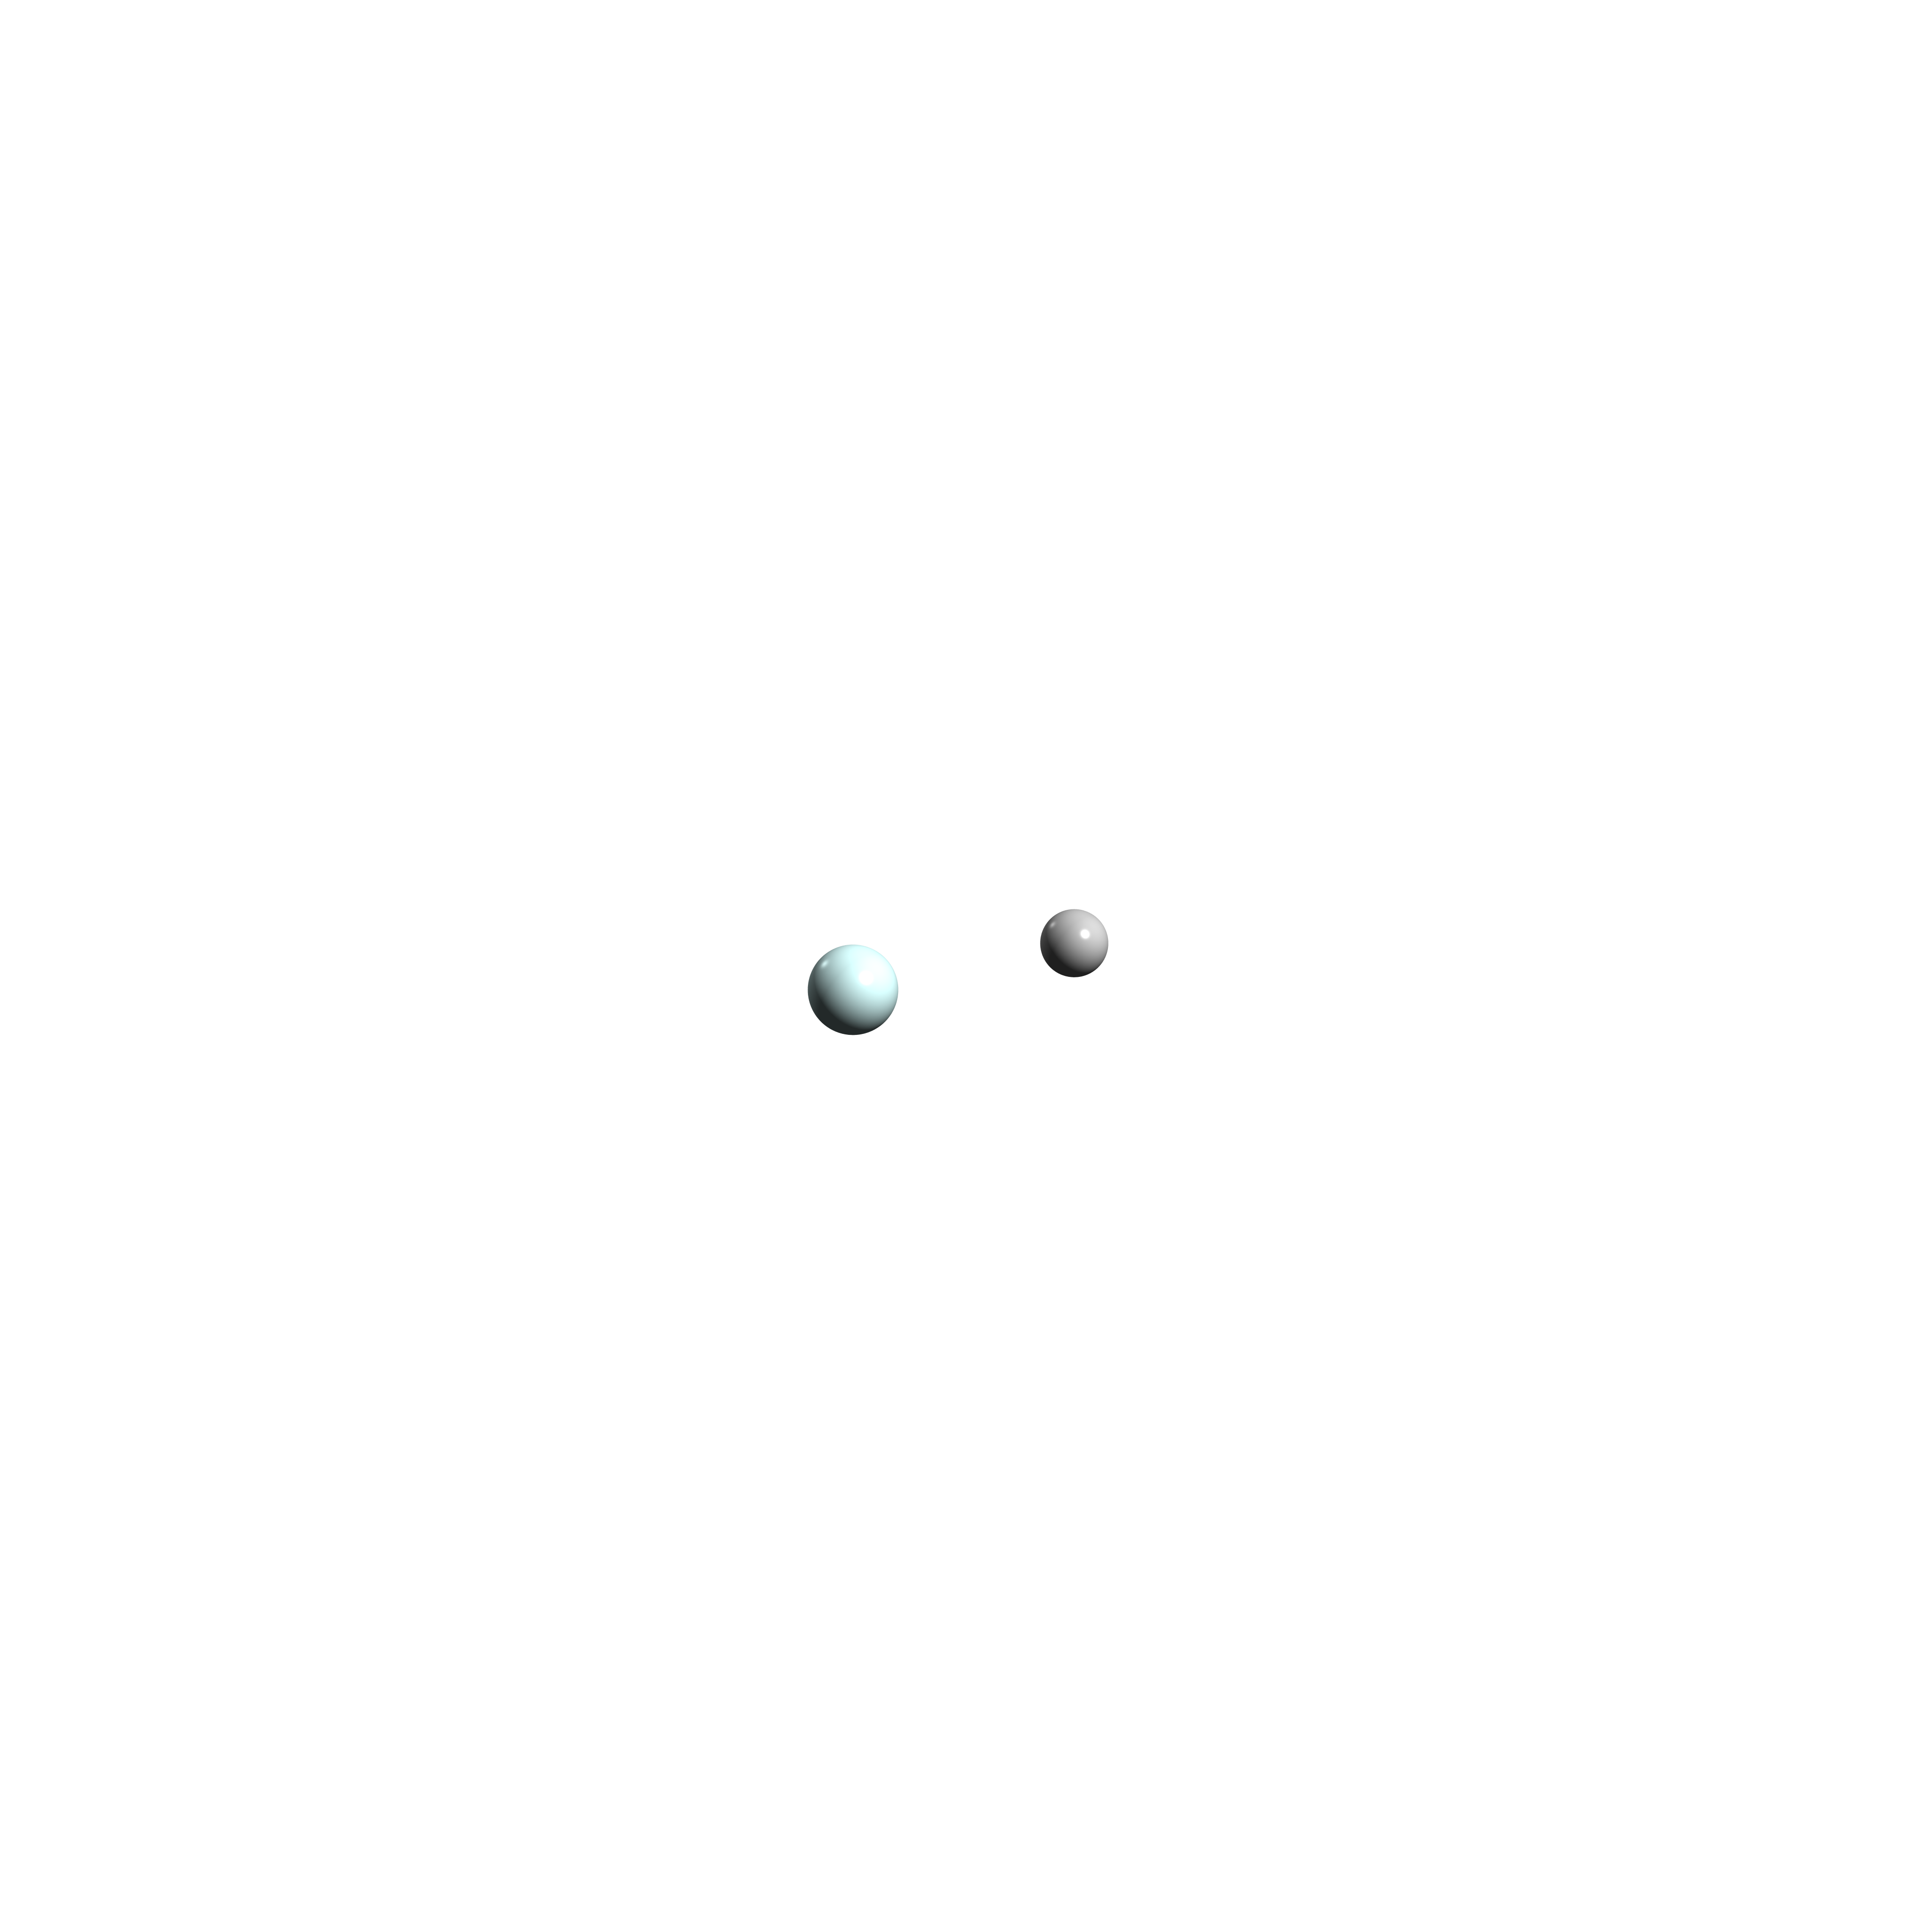
\includegraphics[trim=1400 1400 1400 1400, clip, width=0.24\textwidth]{res/HeH/heh_w.png}
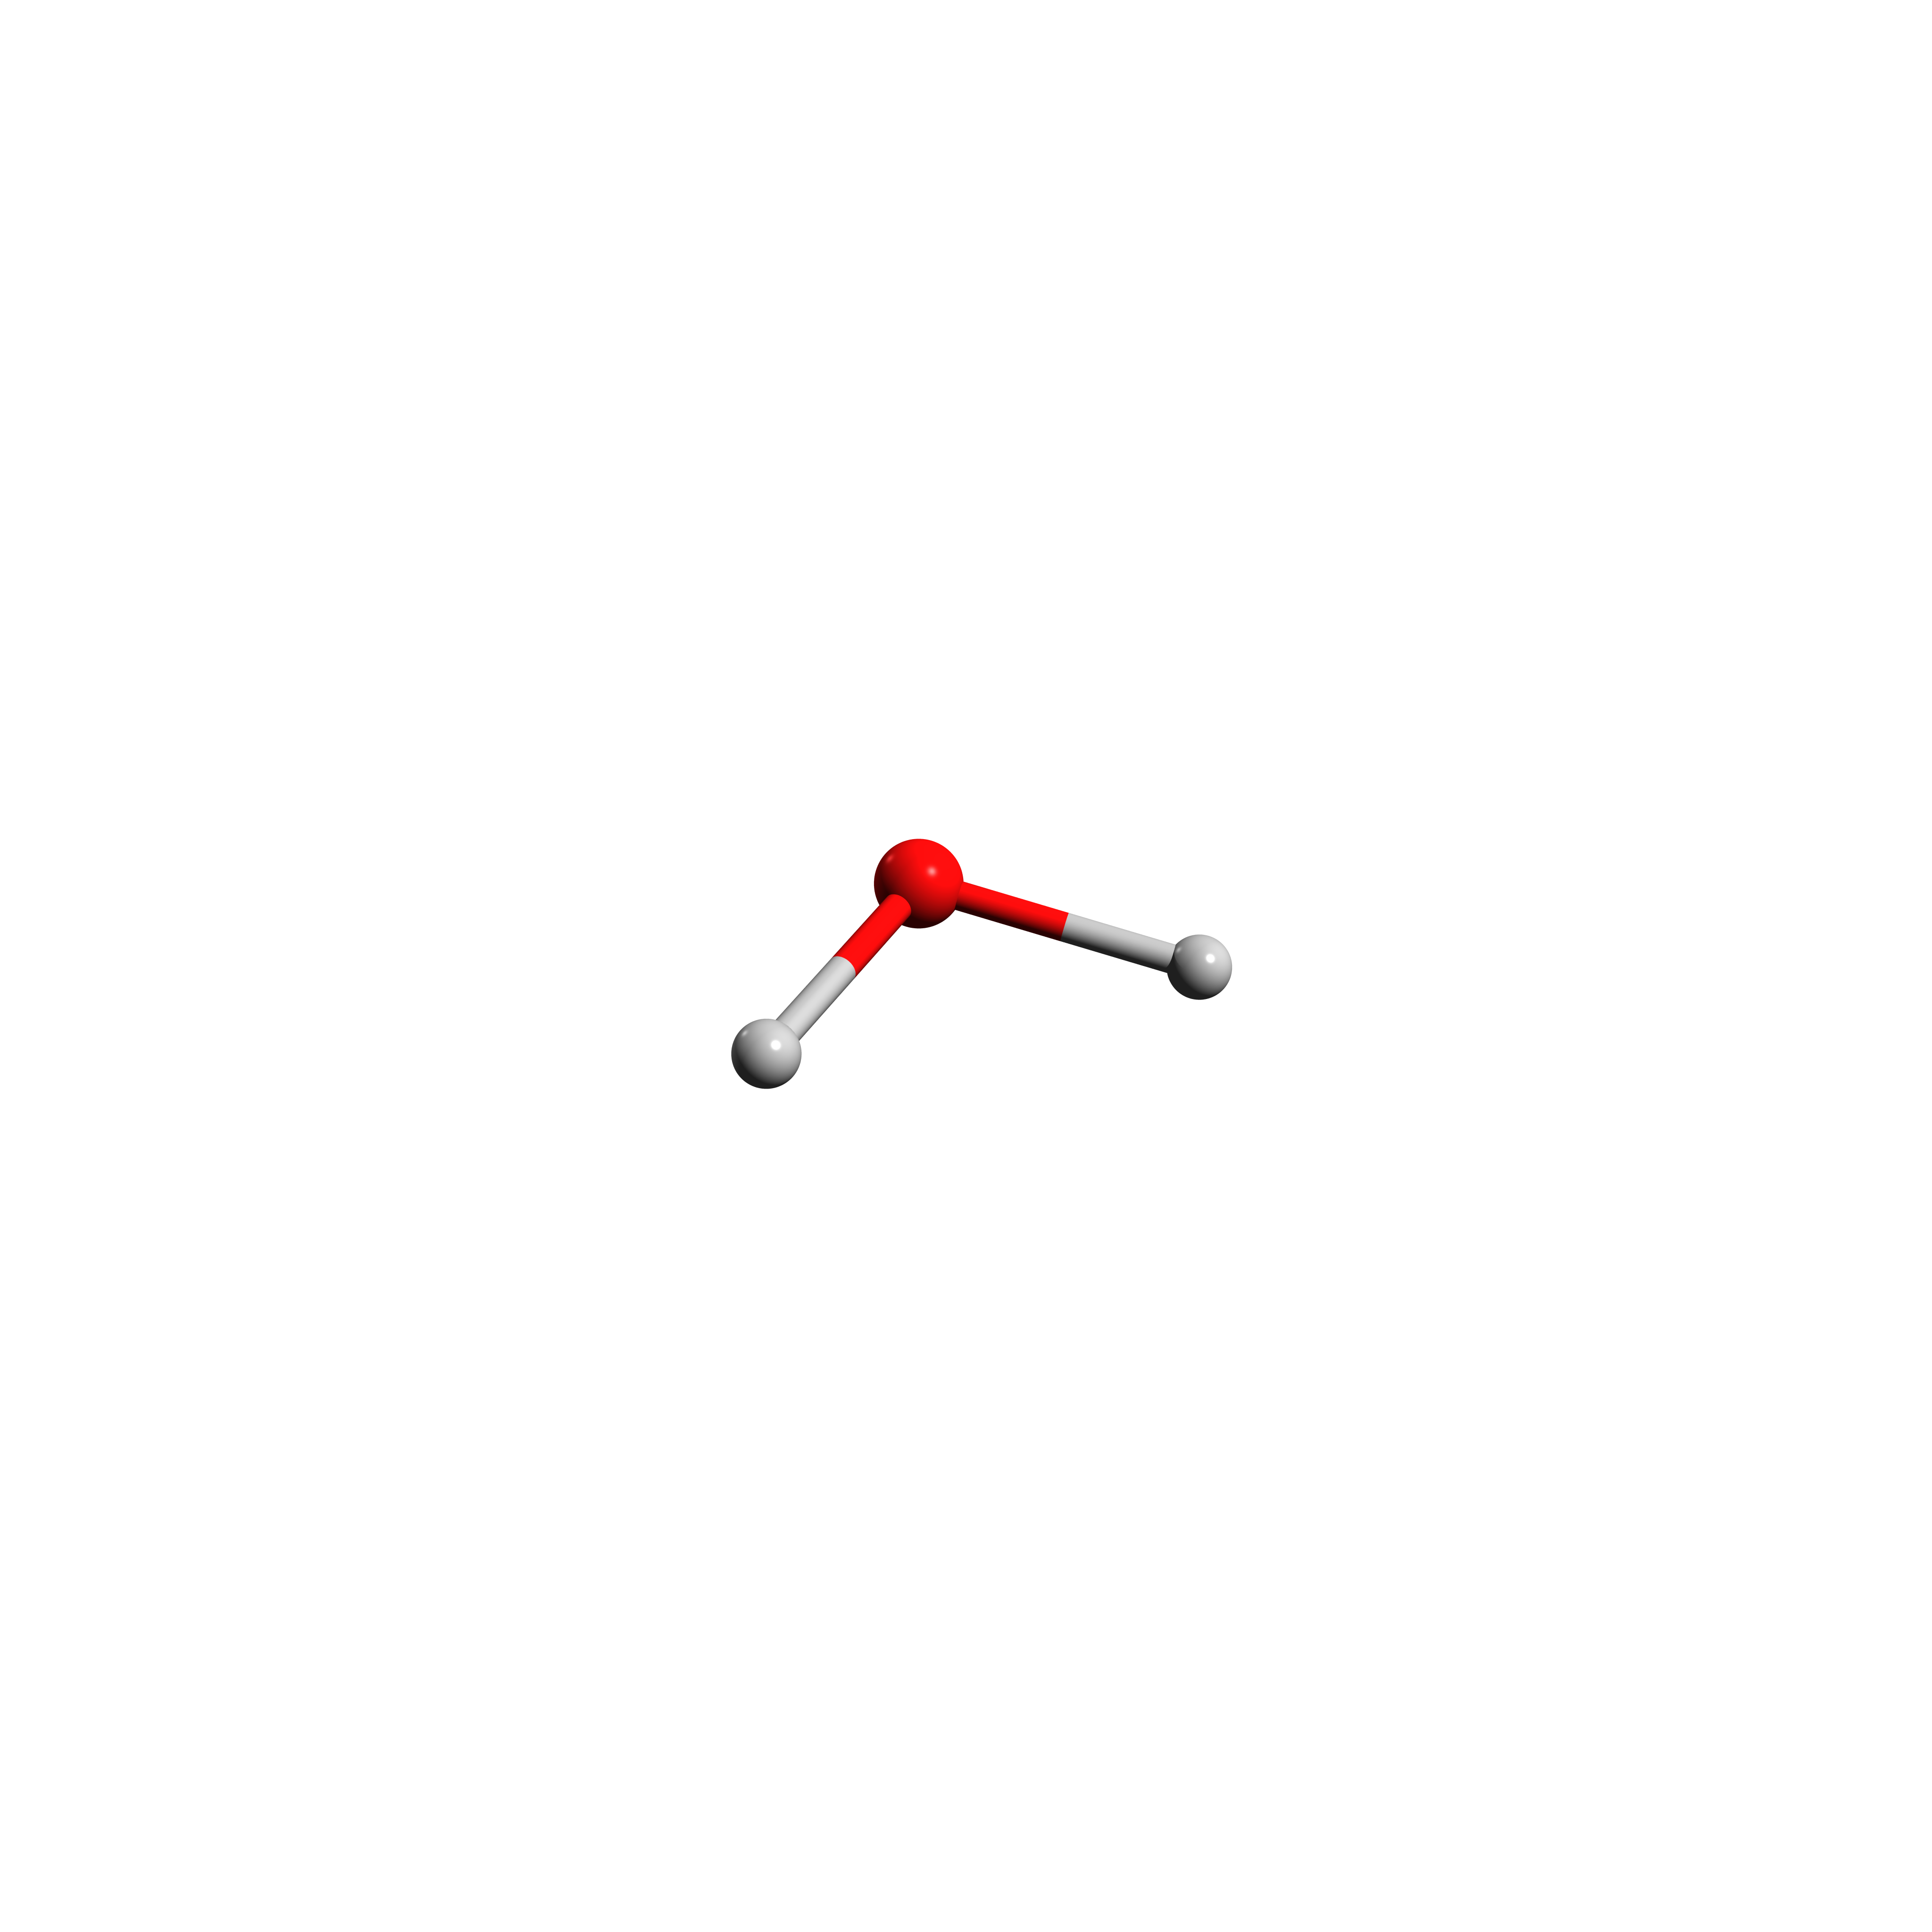
\includegraphics[trim=1400 1400 1400 1400, clip, width=0.24\textwidth]{res/H2O/h2o.png}
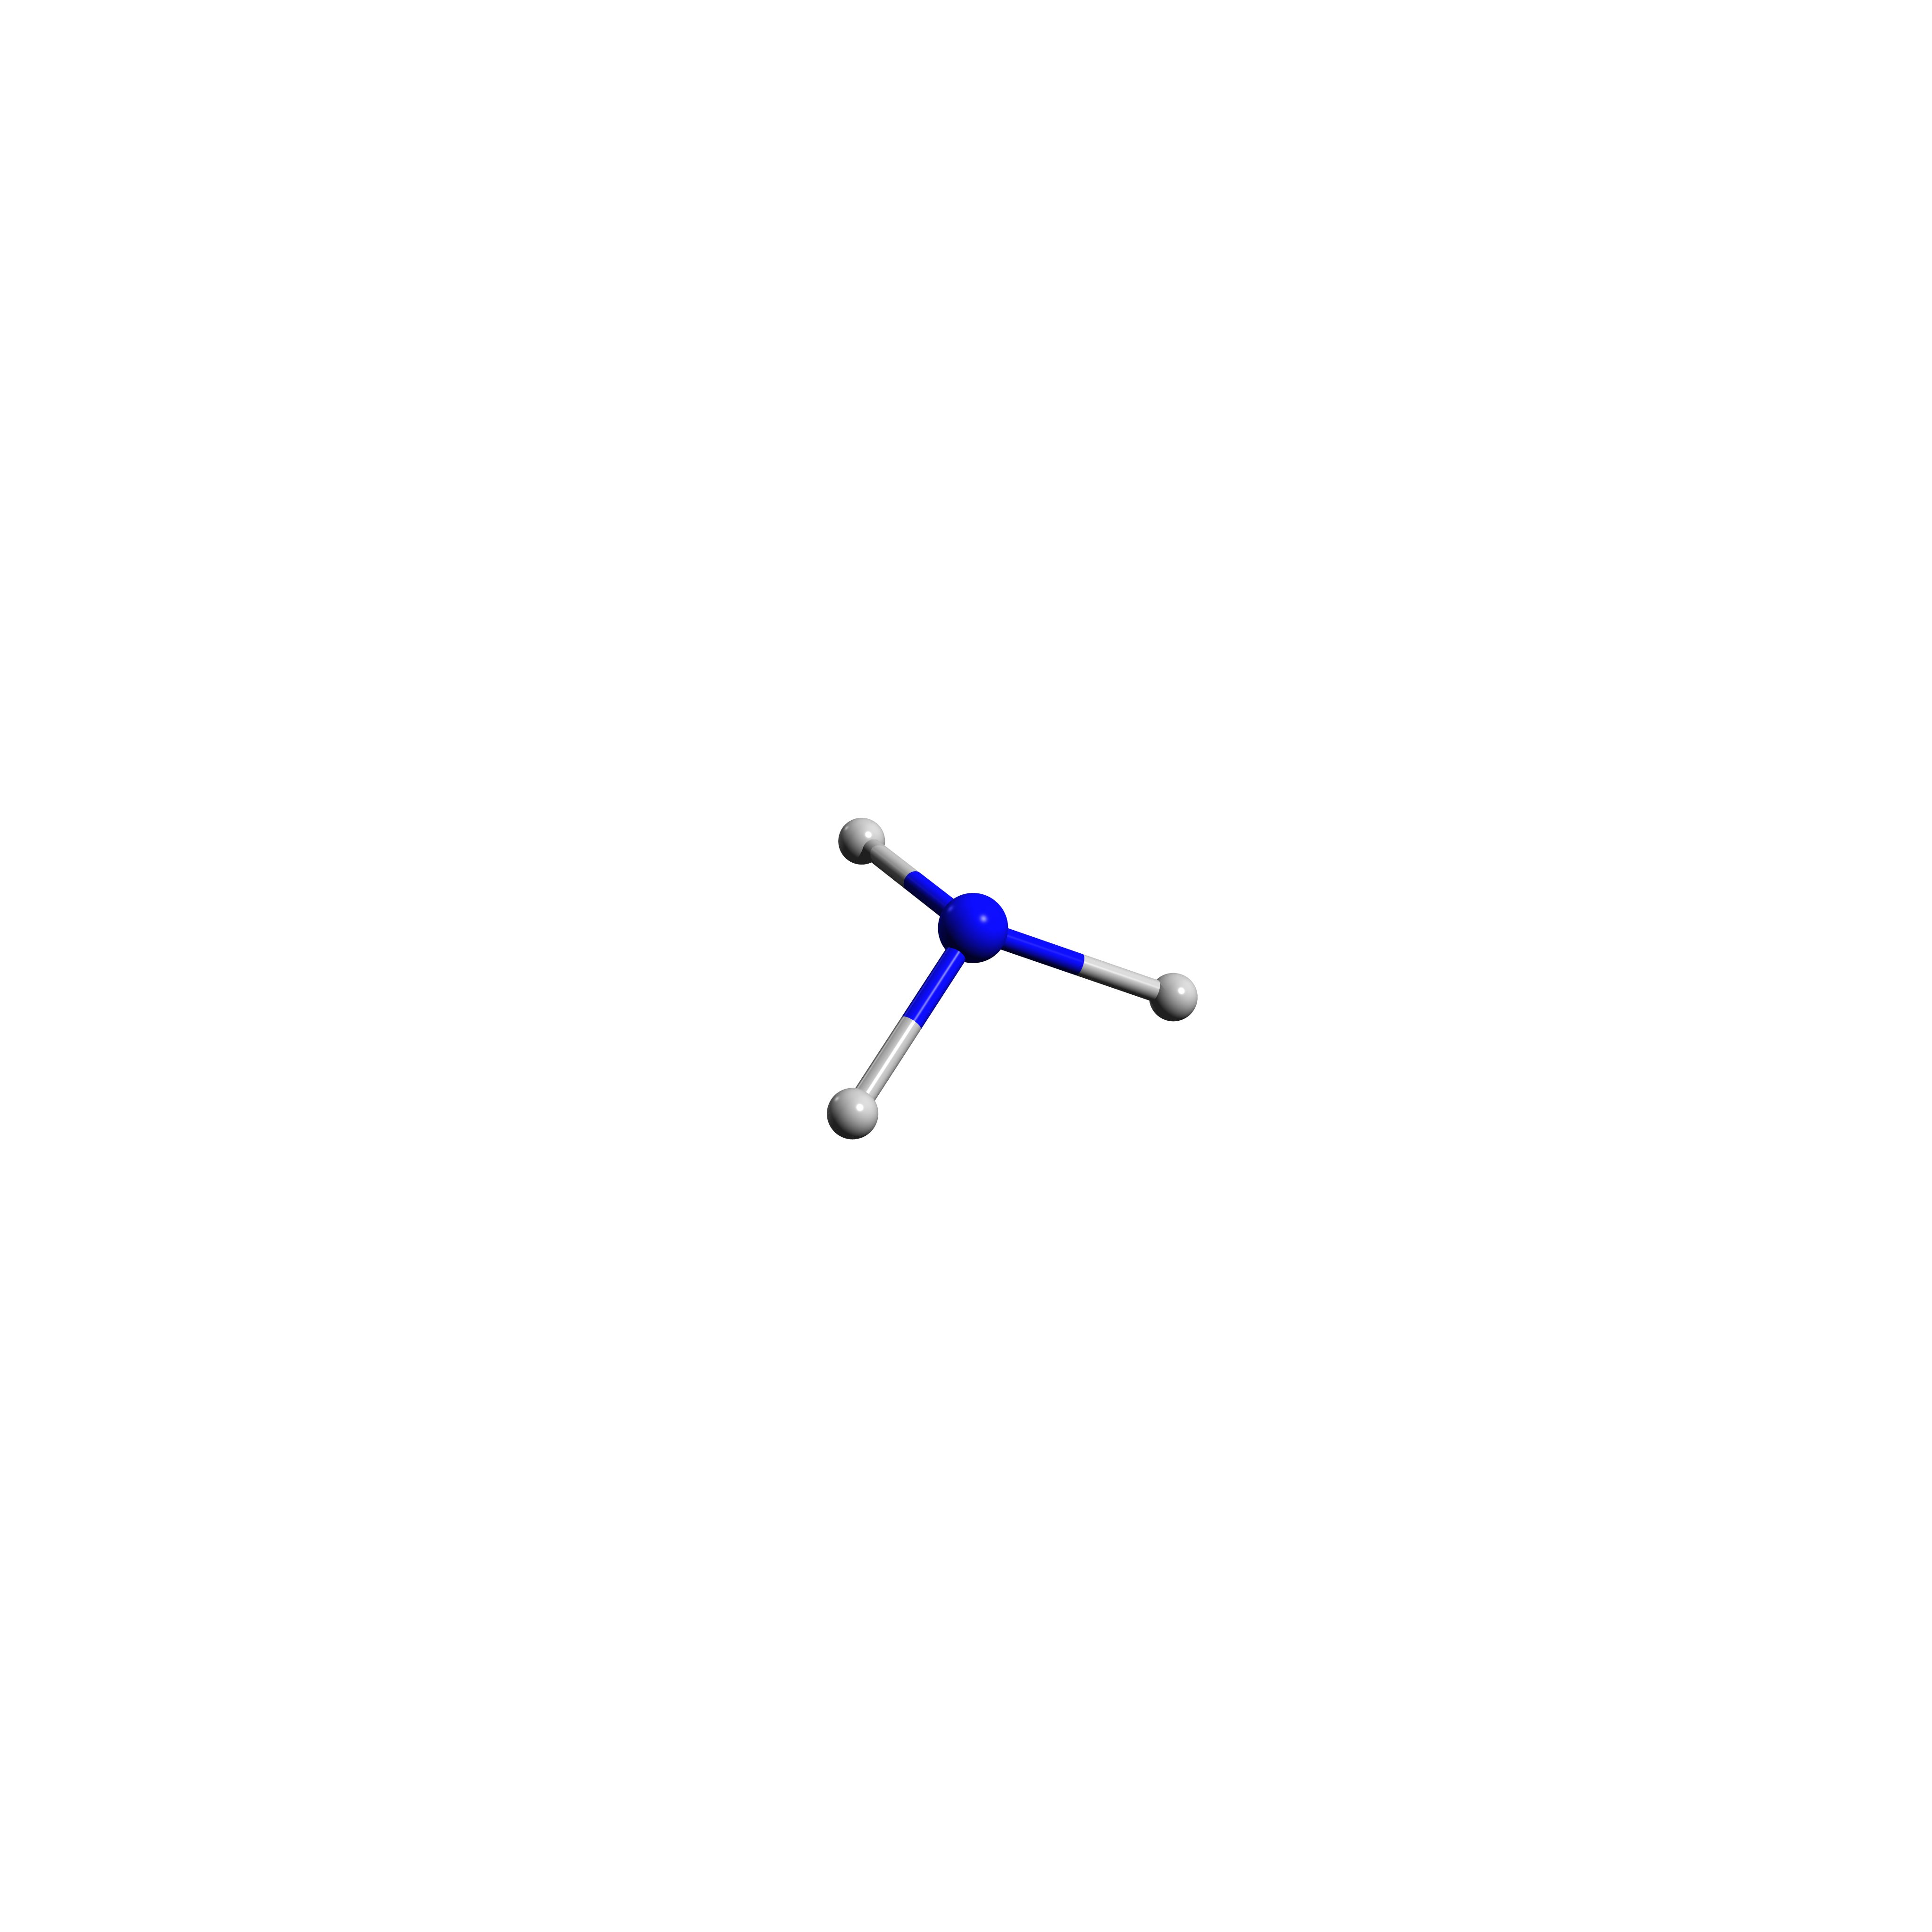
\includegraphics[trim=1400 1400 1400 1400, clip, width=0.24\textwidth]{res/NH3/nh3_d.png}
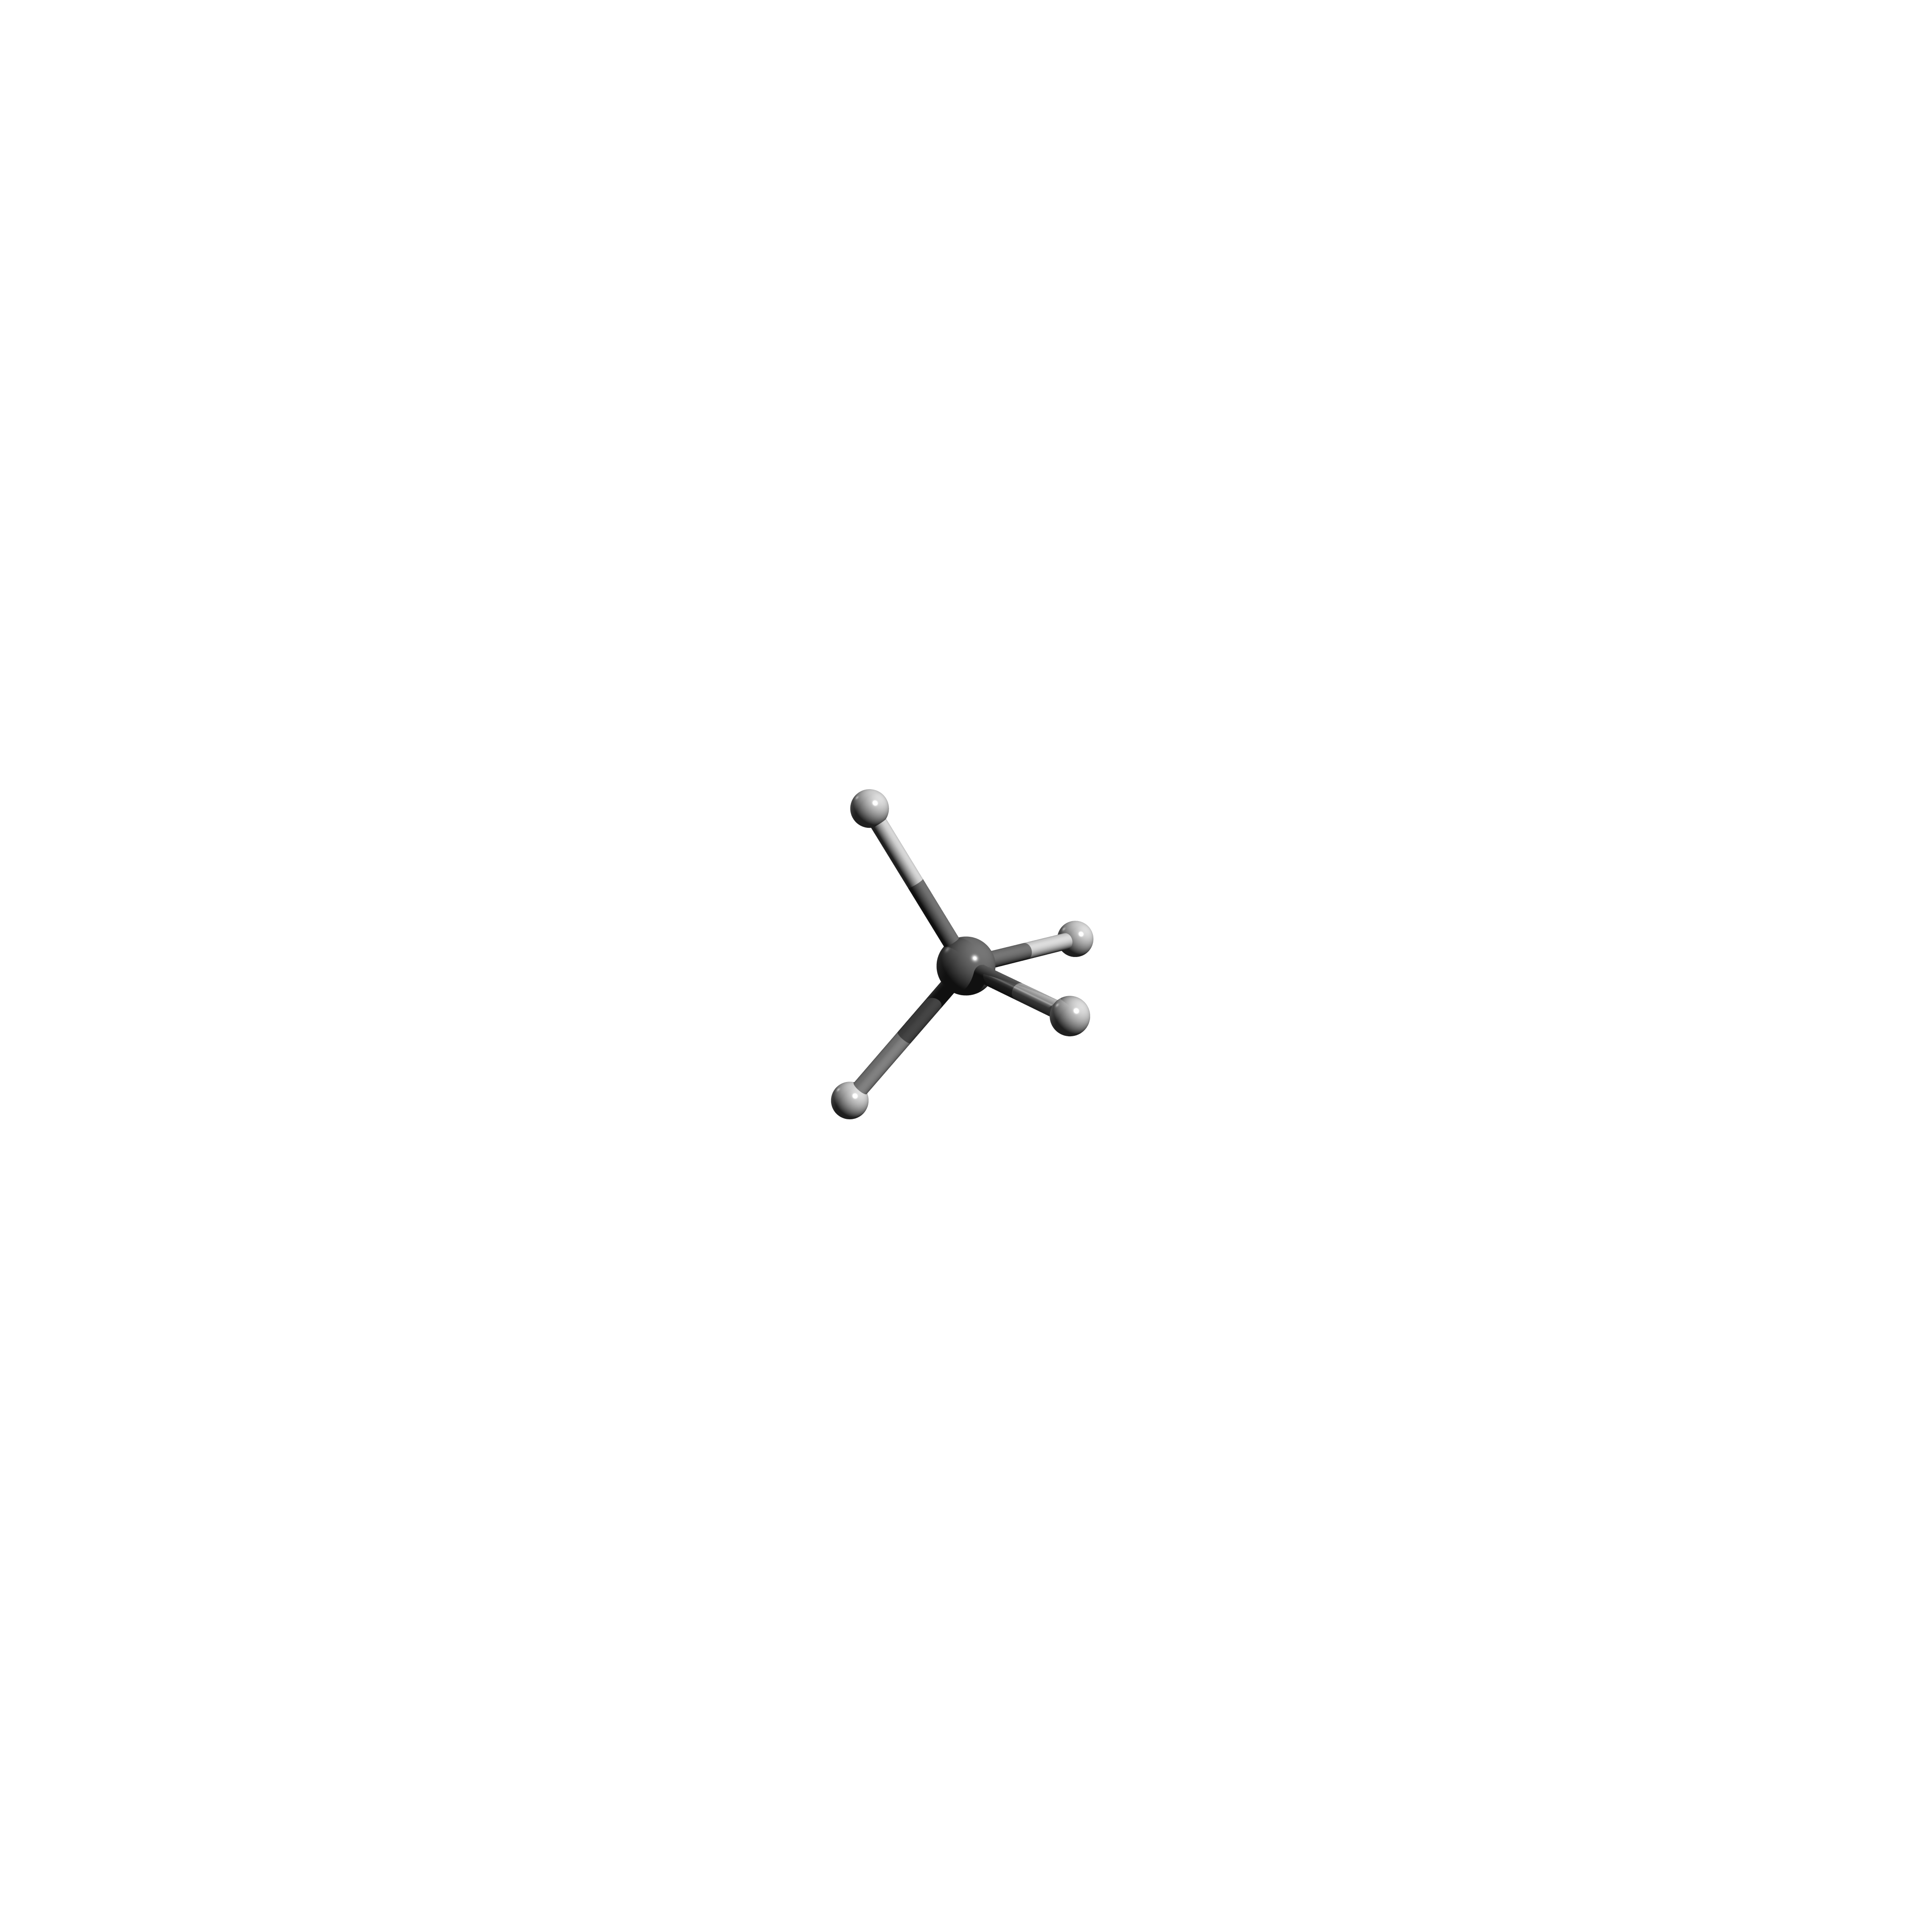
\includegraphics[trim=1400 1400 1400 1400, clip, width=0.24\textwidth]{res/CH4/ch4.png}
\caption{Von links nach rechts: HeH$^+$, H$_2$O, NH$_3$, CH$_4$}\label{molecules}
\end{figure}
Diese Moleküle sind verglichen zu
allen möglichen organischen Verbindungen
relativ einfache Konstrukte und dienen nur zum Testen
der grundlegenden Funktionalität.

Wir berechnen nun für jedes dieser Moleküle die Hartree\-/Fock\-/Energie, 
welche sich aus der elektronischen Energie und
der Internuklearen\-/Abstoßungs\-/Energie zusammen setzt.
Diese Energien vergleichen wir dann mit den
zuverlässigen Ergebnissen aus der NWChem\-/Software.
Es wird lediglich der 6-311+g** Basis\-/Satz verwendet,
dieser ist groß genug, um einigermaßen genaue Berechnungen zu ermöglichen.
Bei den Berechnungen wurden für möglichst identische Startbedingungen gesorgt.

\section{Numerische Experimente}
Diese Hartree\-/Fock\-/Energien (in Hartree) wurden berechnet:
\begin{center}
\begin{tabular}{c|c|c|c|c}
          & HeH$^+$ & H$_2$O & NH$_3$ & CH$_4$\\ \hline
    HFcpp & \unit[-2.88095]{Ha} & \unit[-73.88436]{Ha} & \unit[-54.55853]{Ha} & \unit[-39.01310]{Ha} \\
    NWChem & \unit[-2.92904]{Ha} & \unit[-76.04854]{Ha} & \unit[-56.21346]{Ha} & \unit[-40.20852]{Ha} \\ \hline
    Differenz & \unit[0.04809]{Ha} & \unit[2.16418]{Ha} & \unit[1.65493]{Ha} & \unit[1.19542]{Ha}\\
    Abweichung & $1.64\%$ & $2.85\%$ & $2.94\%$ & $2.97\%$
\end{tabular}
\end{center}

Wie klar zu erkennen ist, sind die berechneten Energien der eigenen Implementierung
im Bereich der Ergebnisse der NWChem\-/Software. Es lässt sich schlussfolgern,
dass die Implementierung korrekt ist.
Die deutlich besseren Ergebnisse der NWChem-Software
trotz gleicher Startbedingungen sind sehr wahrscheinlich 
auf Unterschiede in der Implementierung zurückzuführen,
wie zum Beispiel auf den Einsatz zusätzlicher Optimierungen.

Die Hartree\-/Fock\-/Energien sind jedoch nicht die einzigen Ergebnisse,
wir erhalten noch die Orbital\-/Funktionen und deren zugehörigen Energien.
Diese lassen sich in einem Isoflächen\-/Plot gut darstellen.
Die nachstehenden Grafiken wurden mithilfe der Programme Avogadro \cite{avogadro}
und POV-Ray \cite{povray} erzeugt.
\begin{enumerate}
\item Heliumhydridion (HeH$^+$):
\begin{figure}[H]
\centering
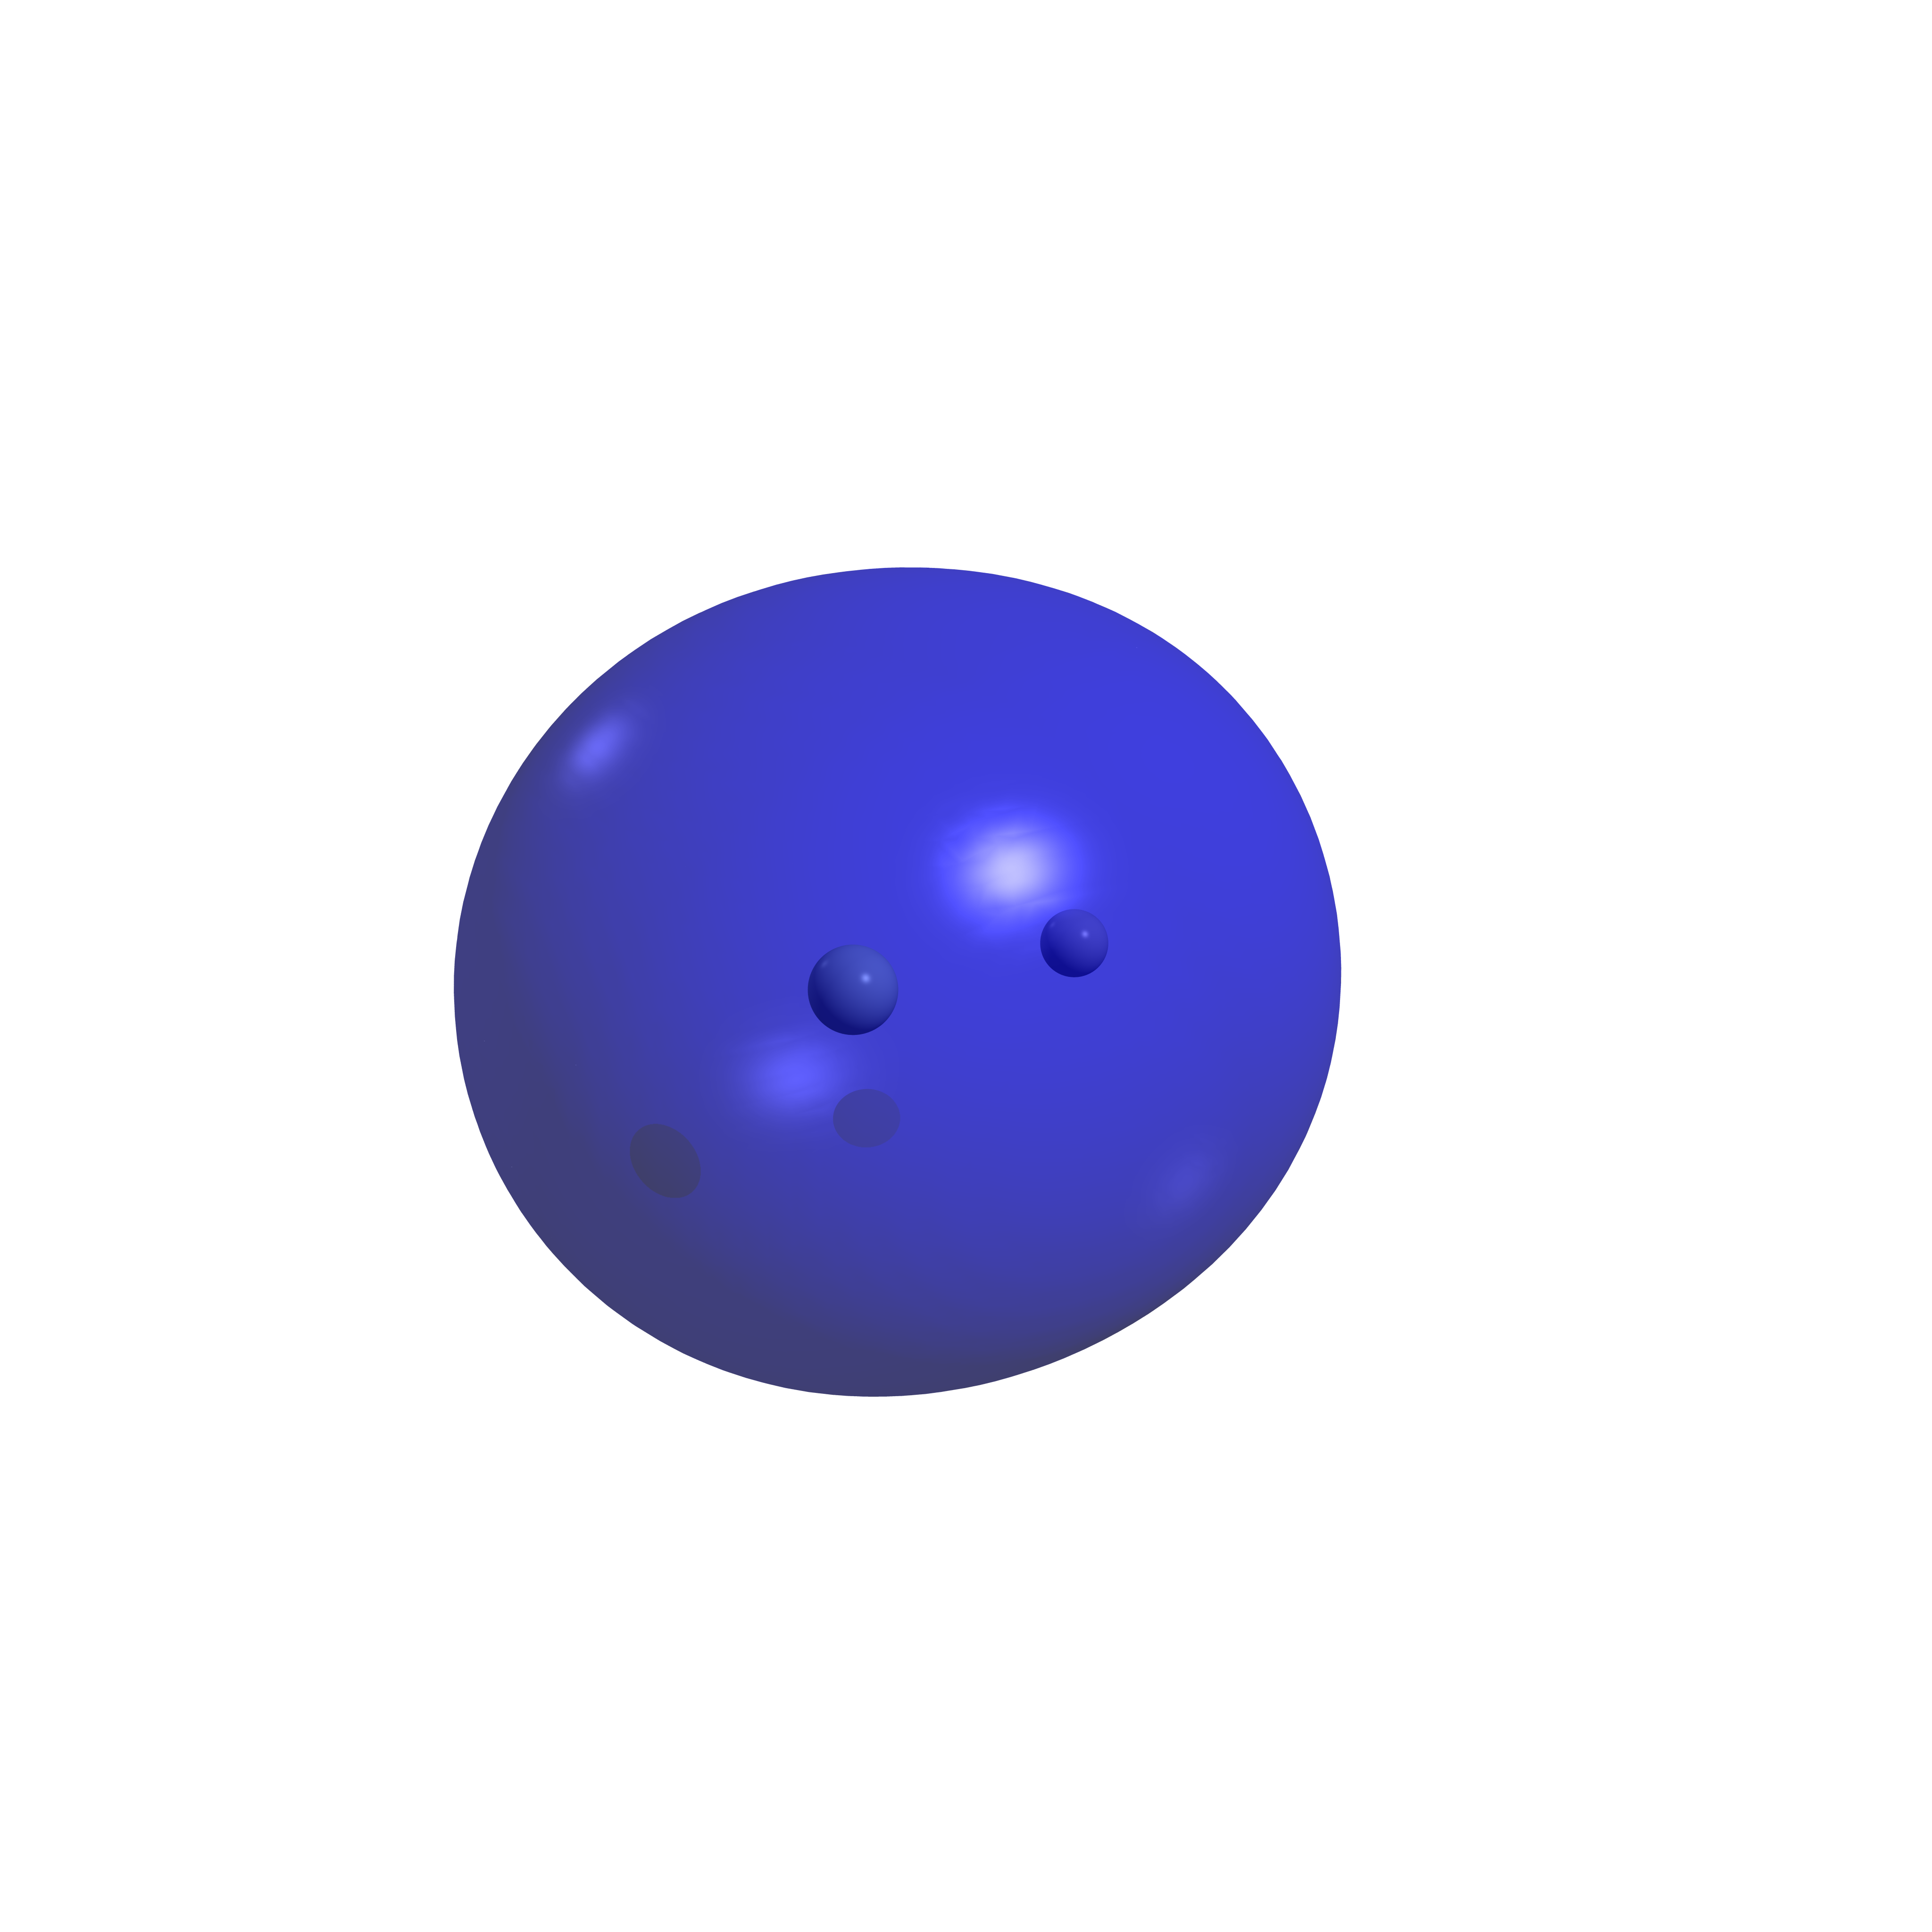
\includegraphics[trim=300 300 300 300, clip, width=0.45\textwidth]{res/HeH/heh_w0.png}
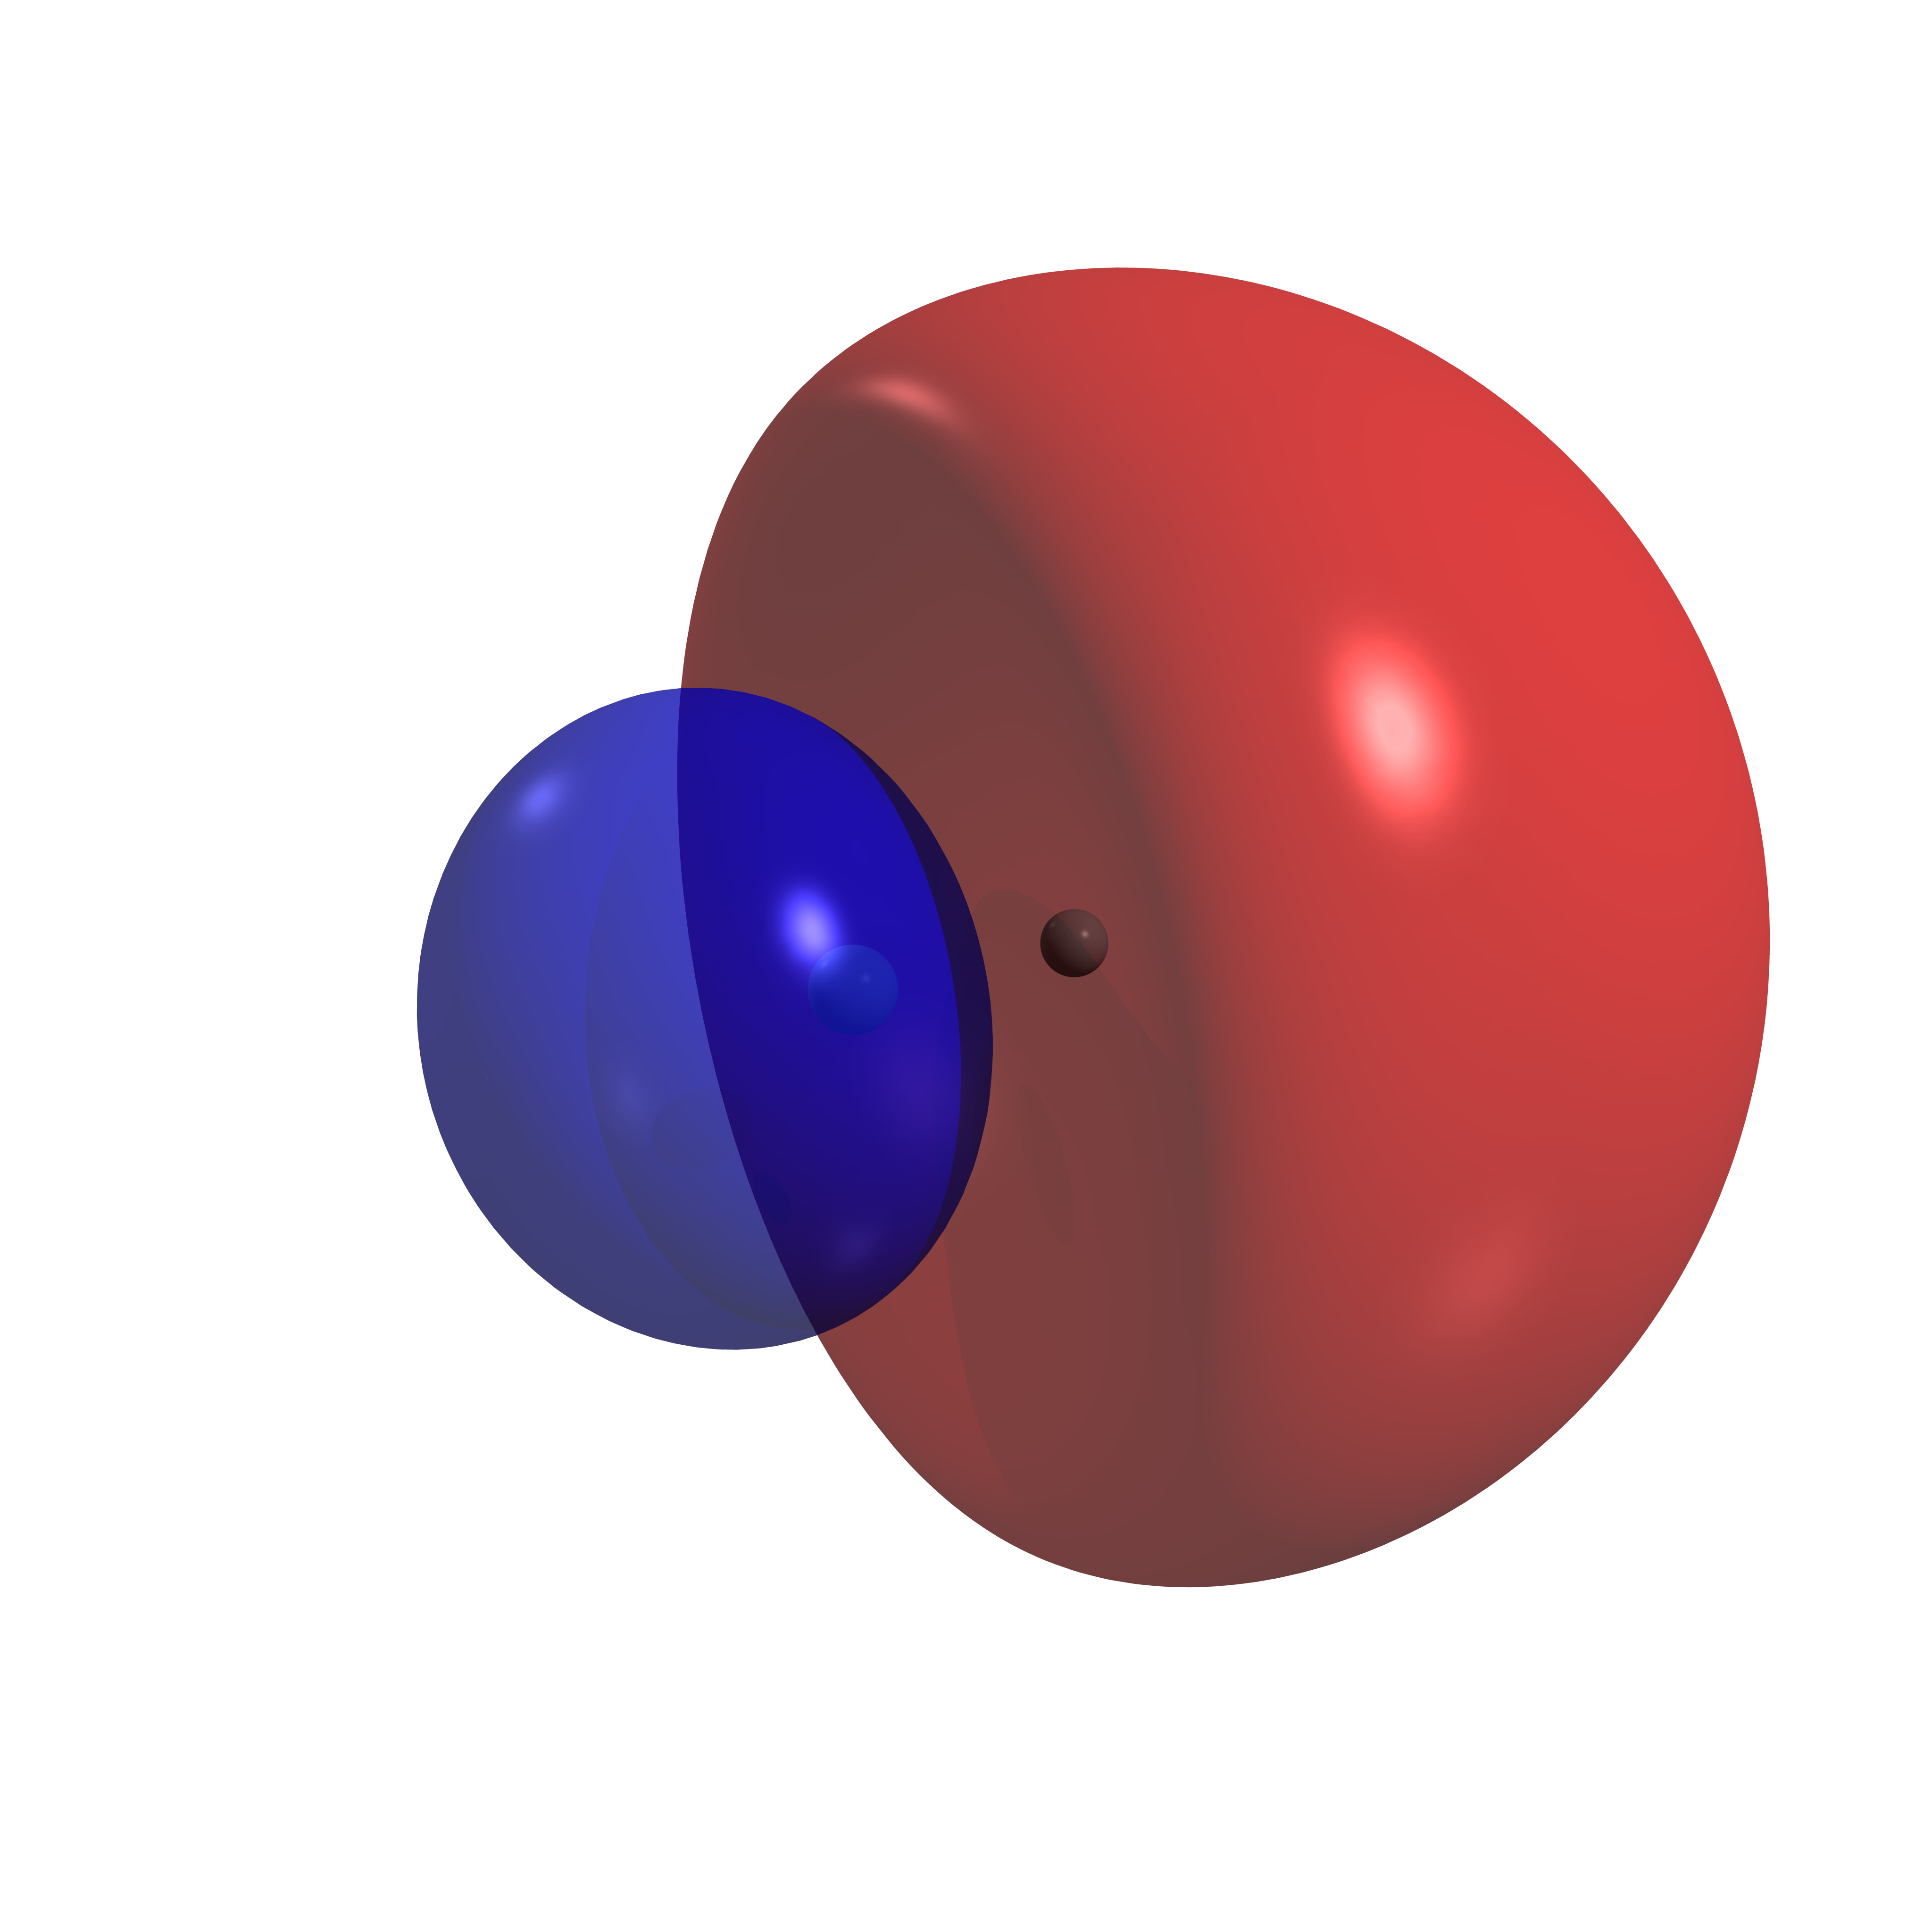
\includegraphics[trim=300 300 300 300, clip, width=0.45\textwidth]{res/HeH/heh_w1.png}
\caption{Die ersten zwei Orbitale des HeH$^+$\-/Moleküls,
nach aufsteigender Energie sortiert.
\textcolor{blue}{$\blacksquare$} positiv,
\textcolor{red}{$\blacksquare$} negativ.}\label{heh_orbitals}
\end{figure}

\newpage
\item Wasser (H$_2$O):
\begin{figure}[H]
\centering
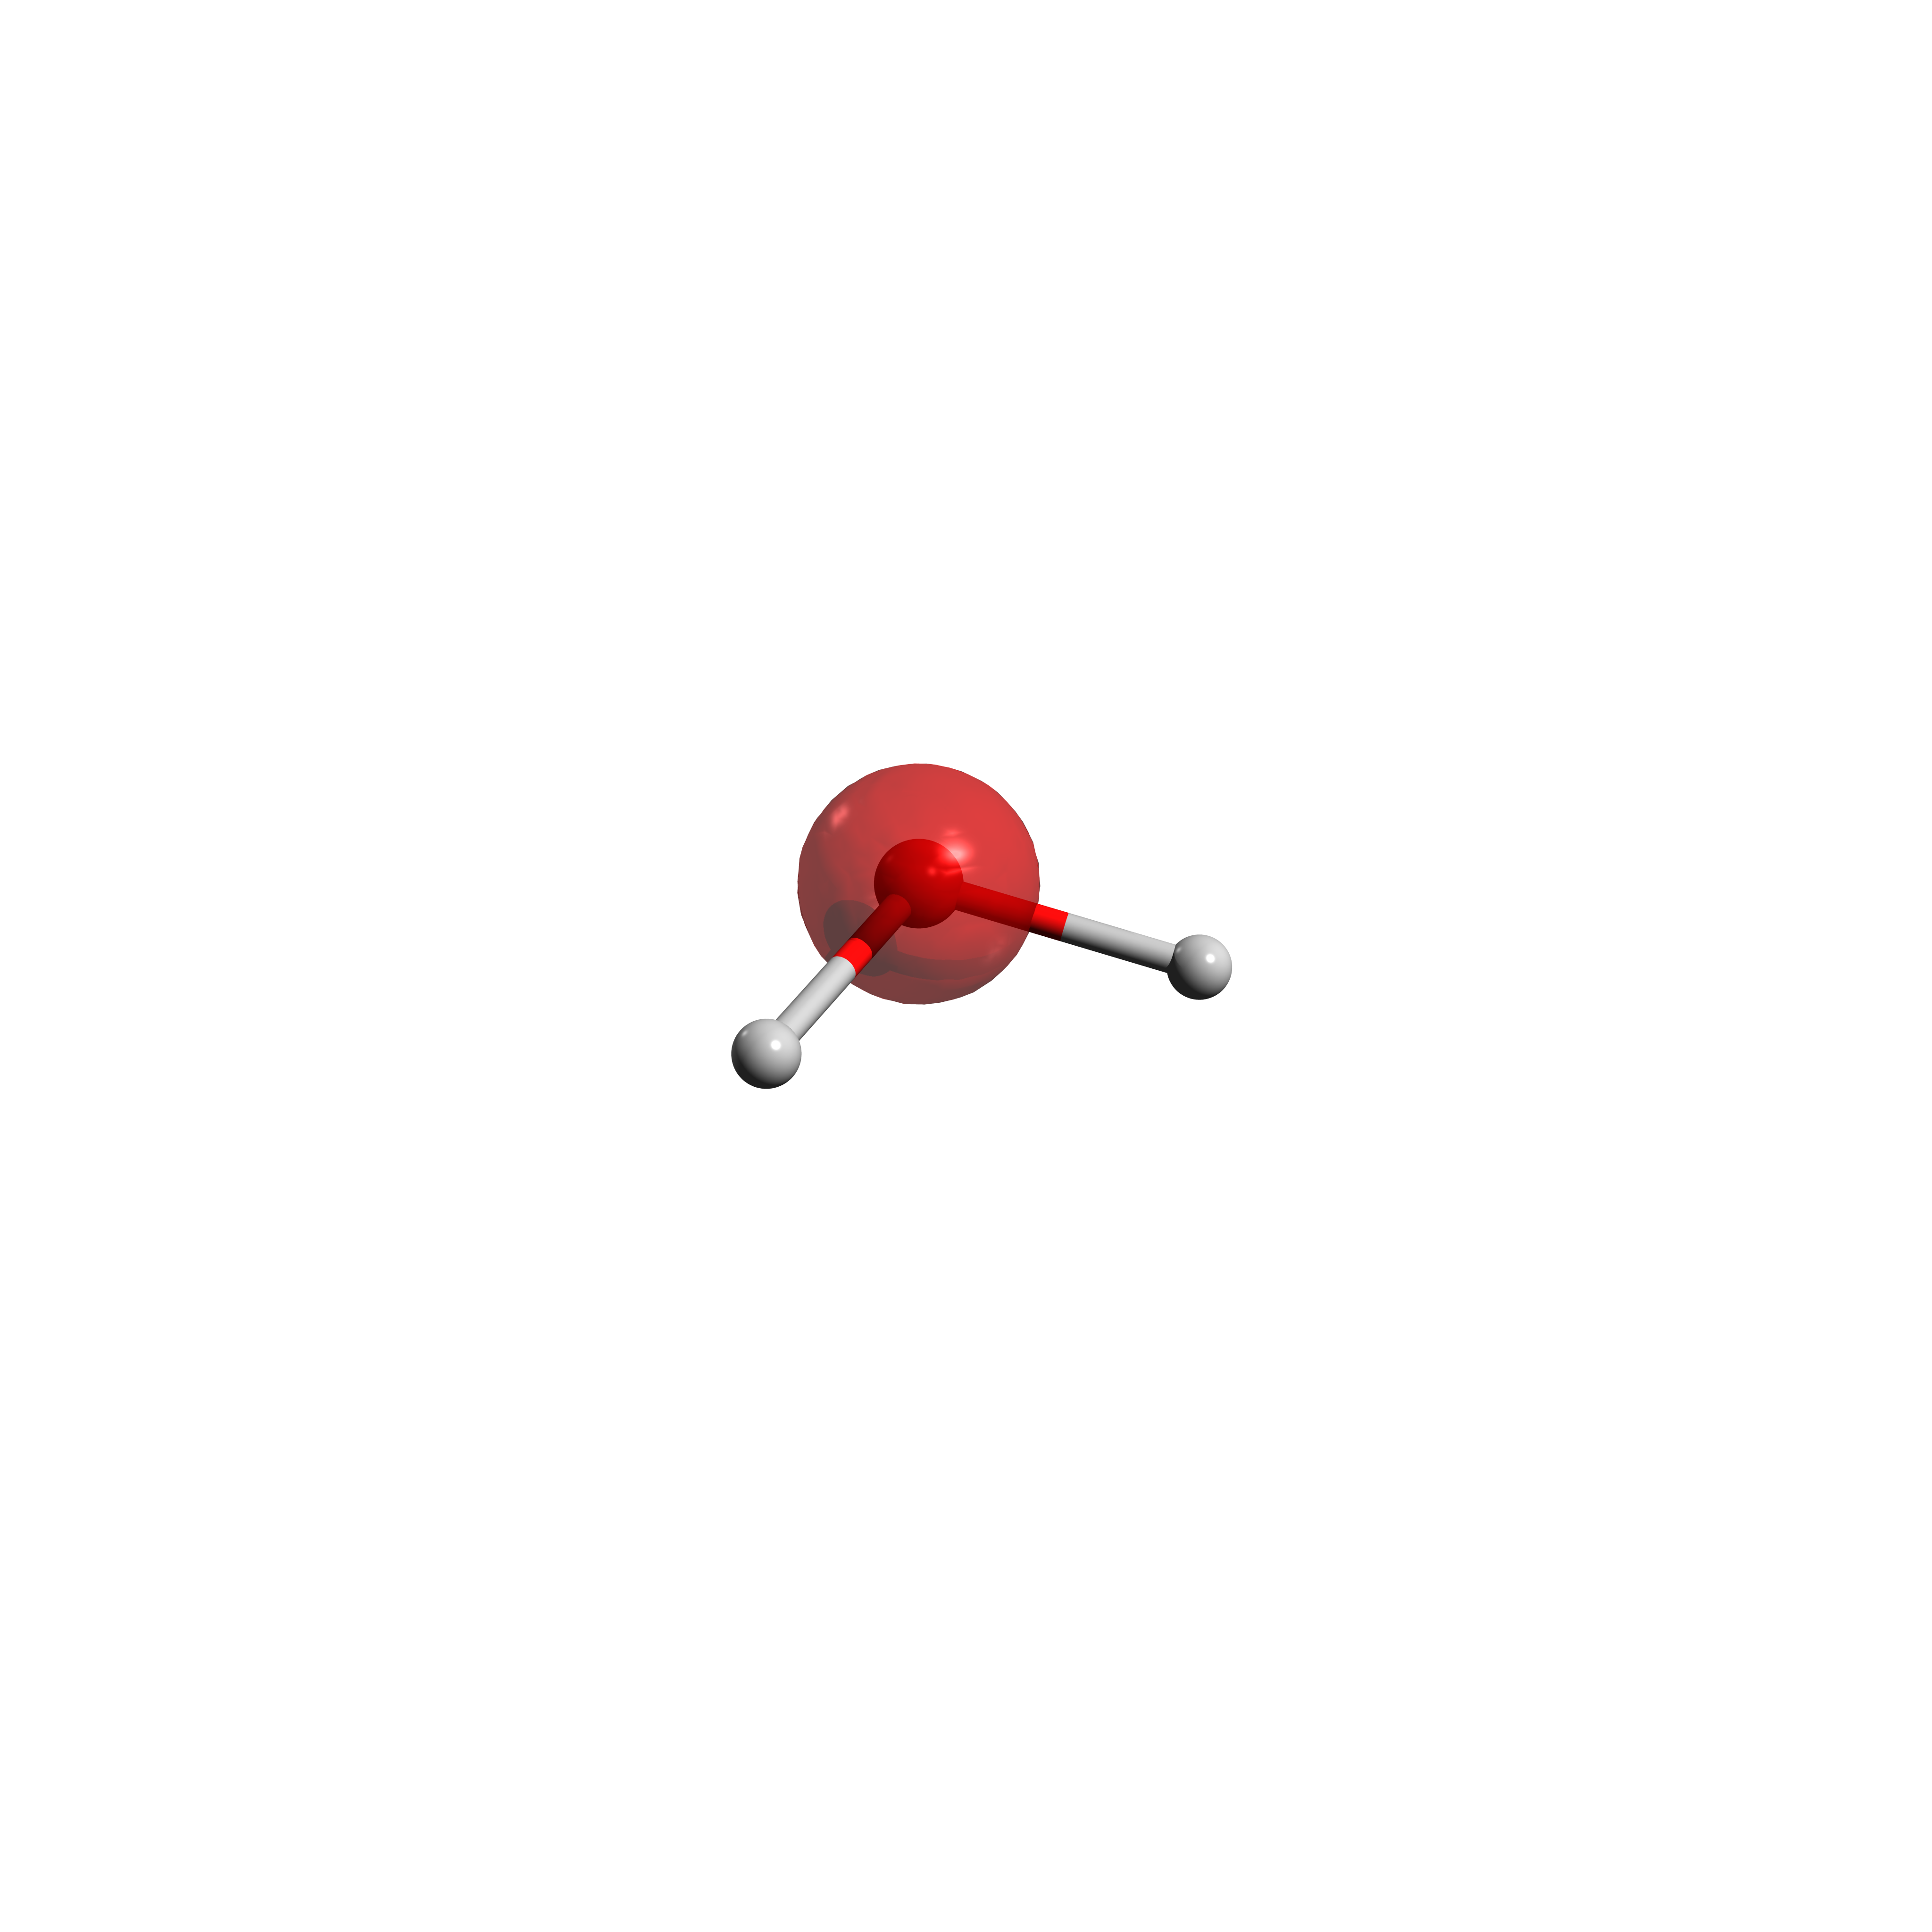
\includegraphics[trim=700 800 700 600, clip, width=0.45\textwidth]{res/H2O/h2o_w0.png}
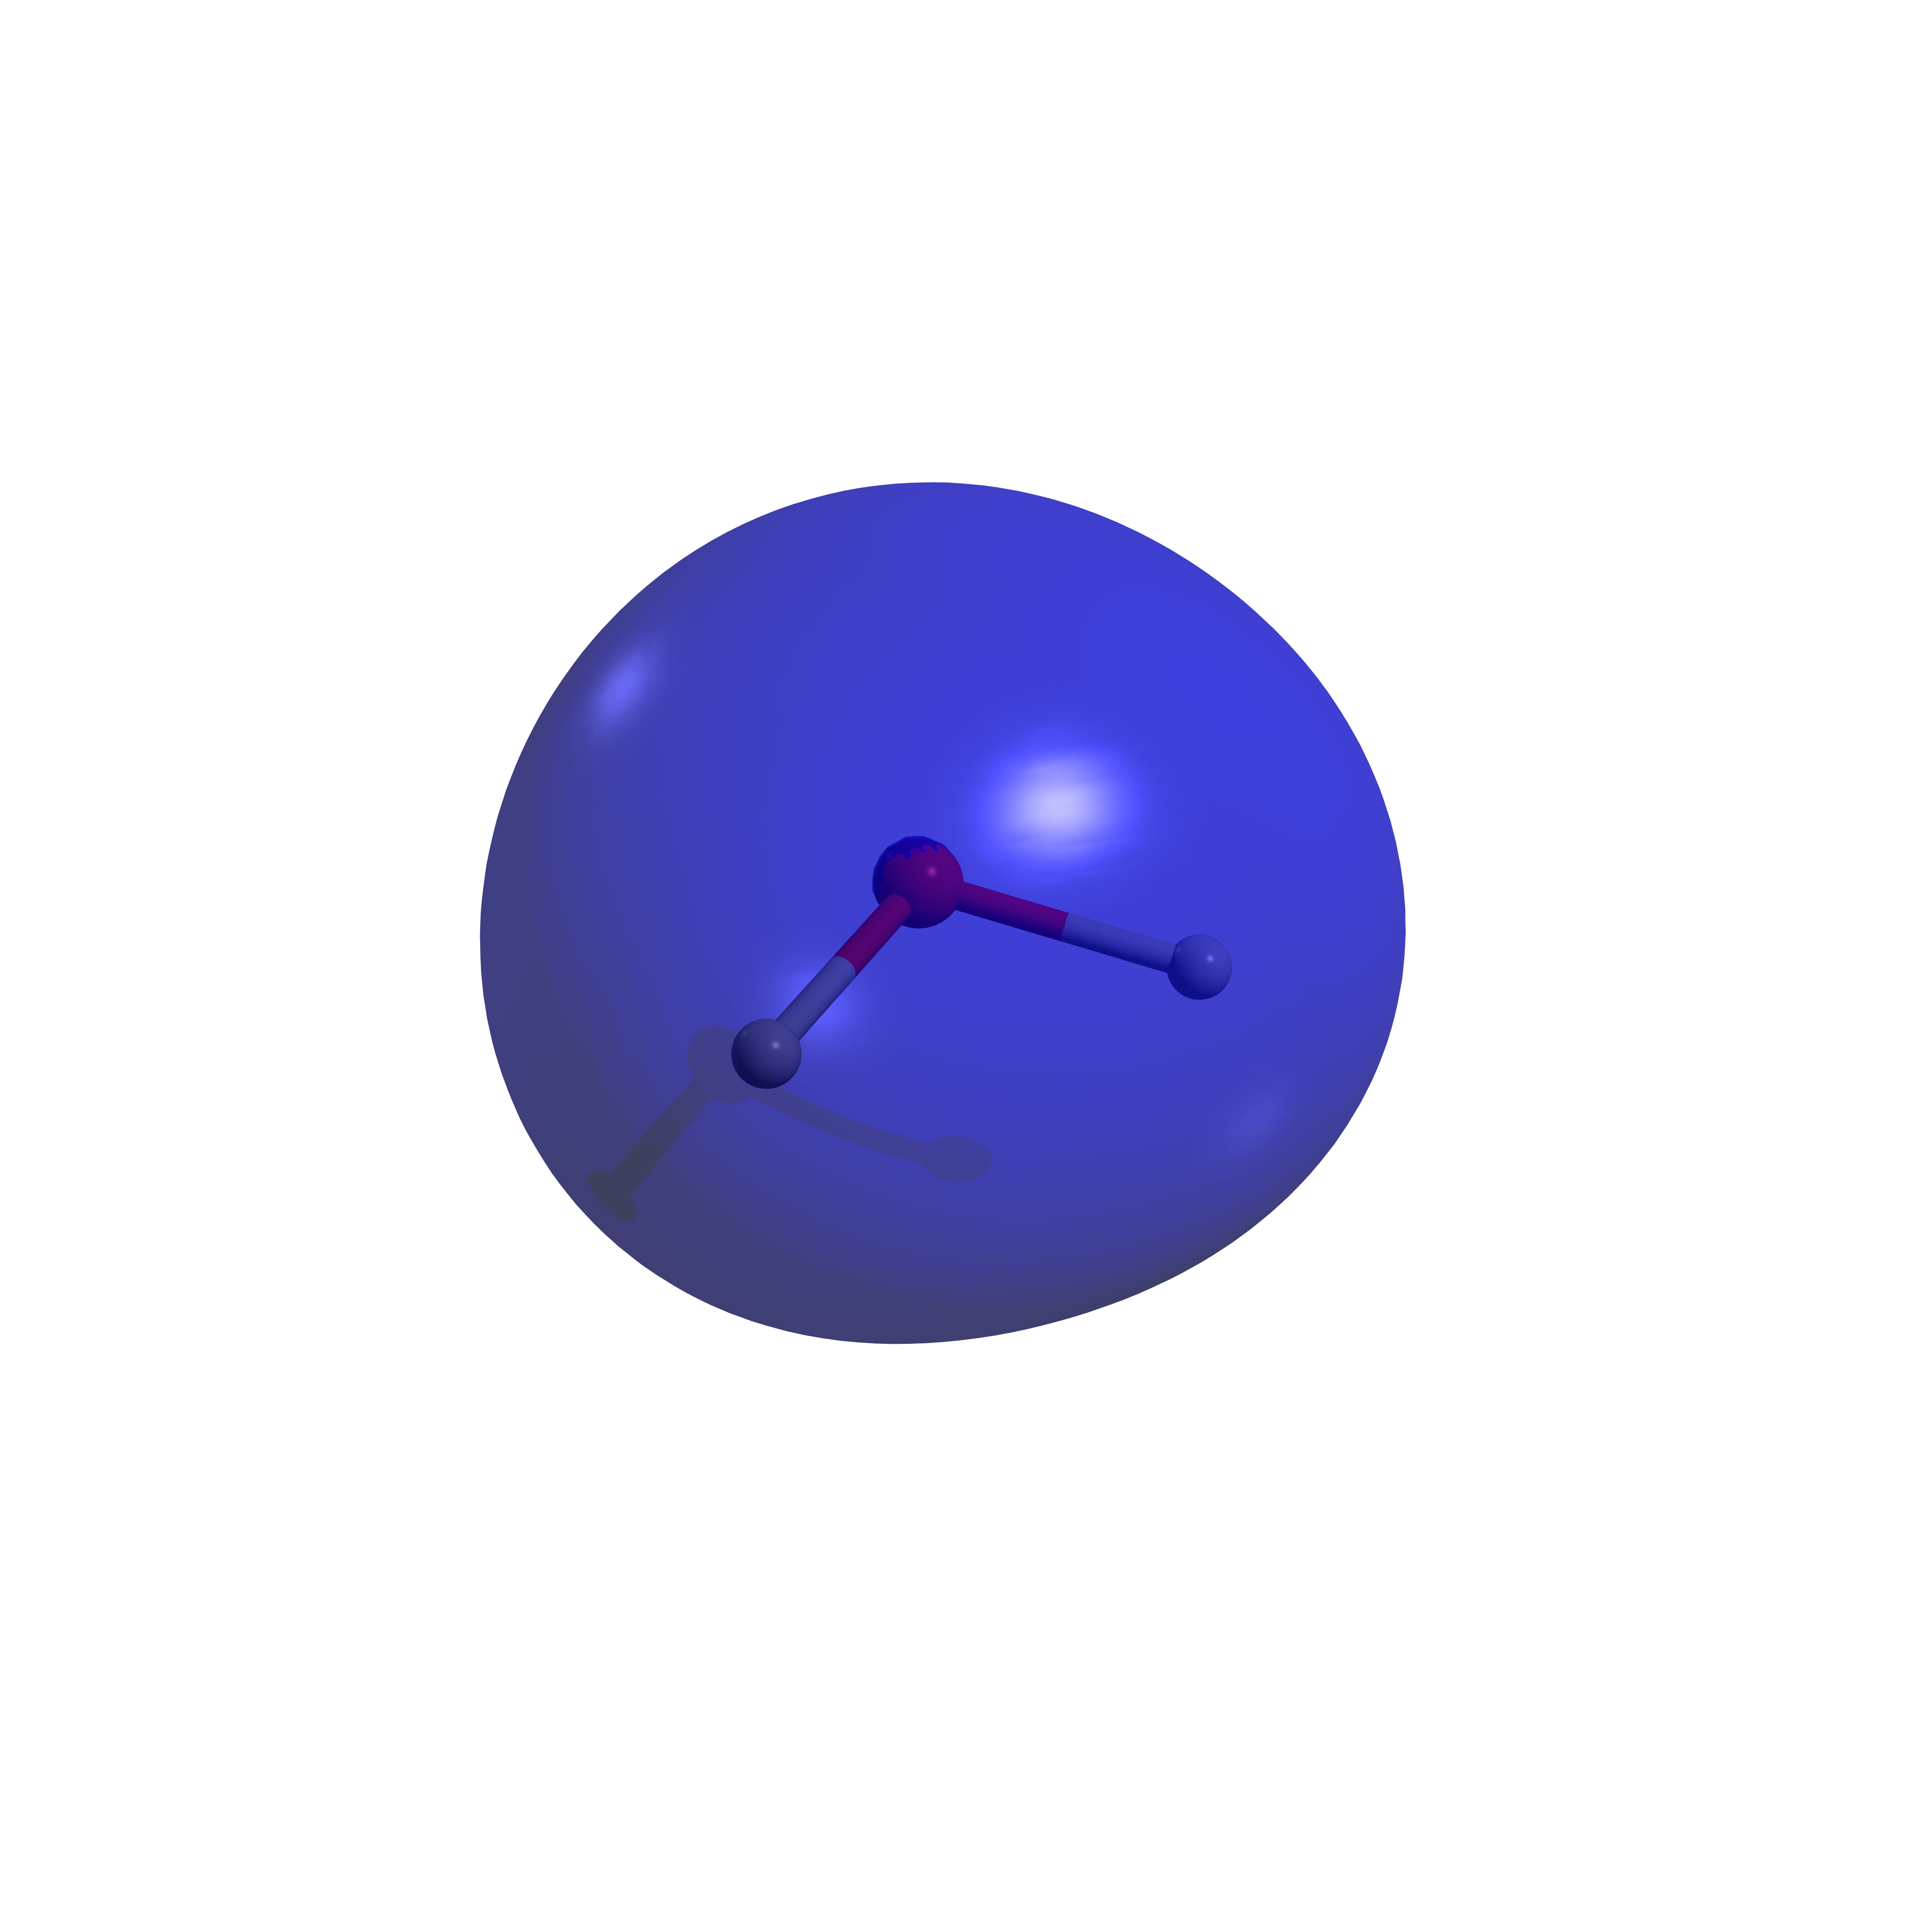
\includegraphics[trim=700 800 700 600, clip, width=0.45\textwidth]{res/H2O/h2o_w1.png}\\
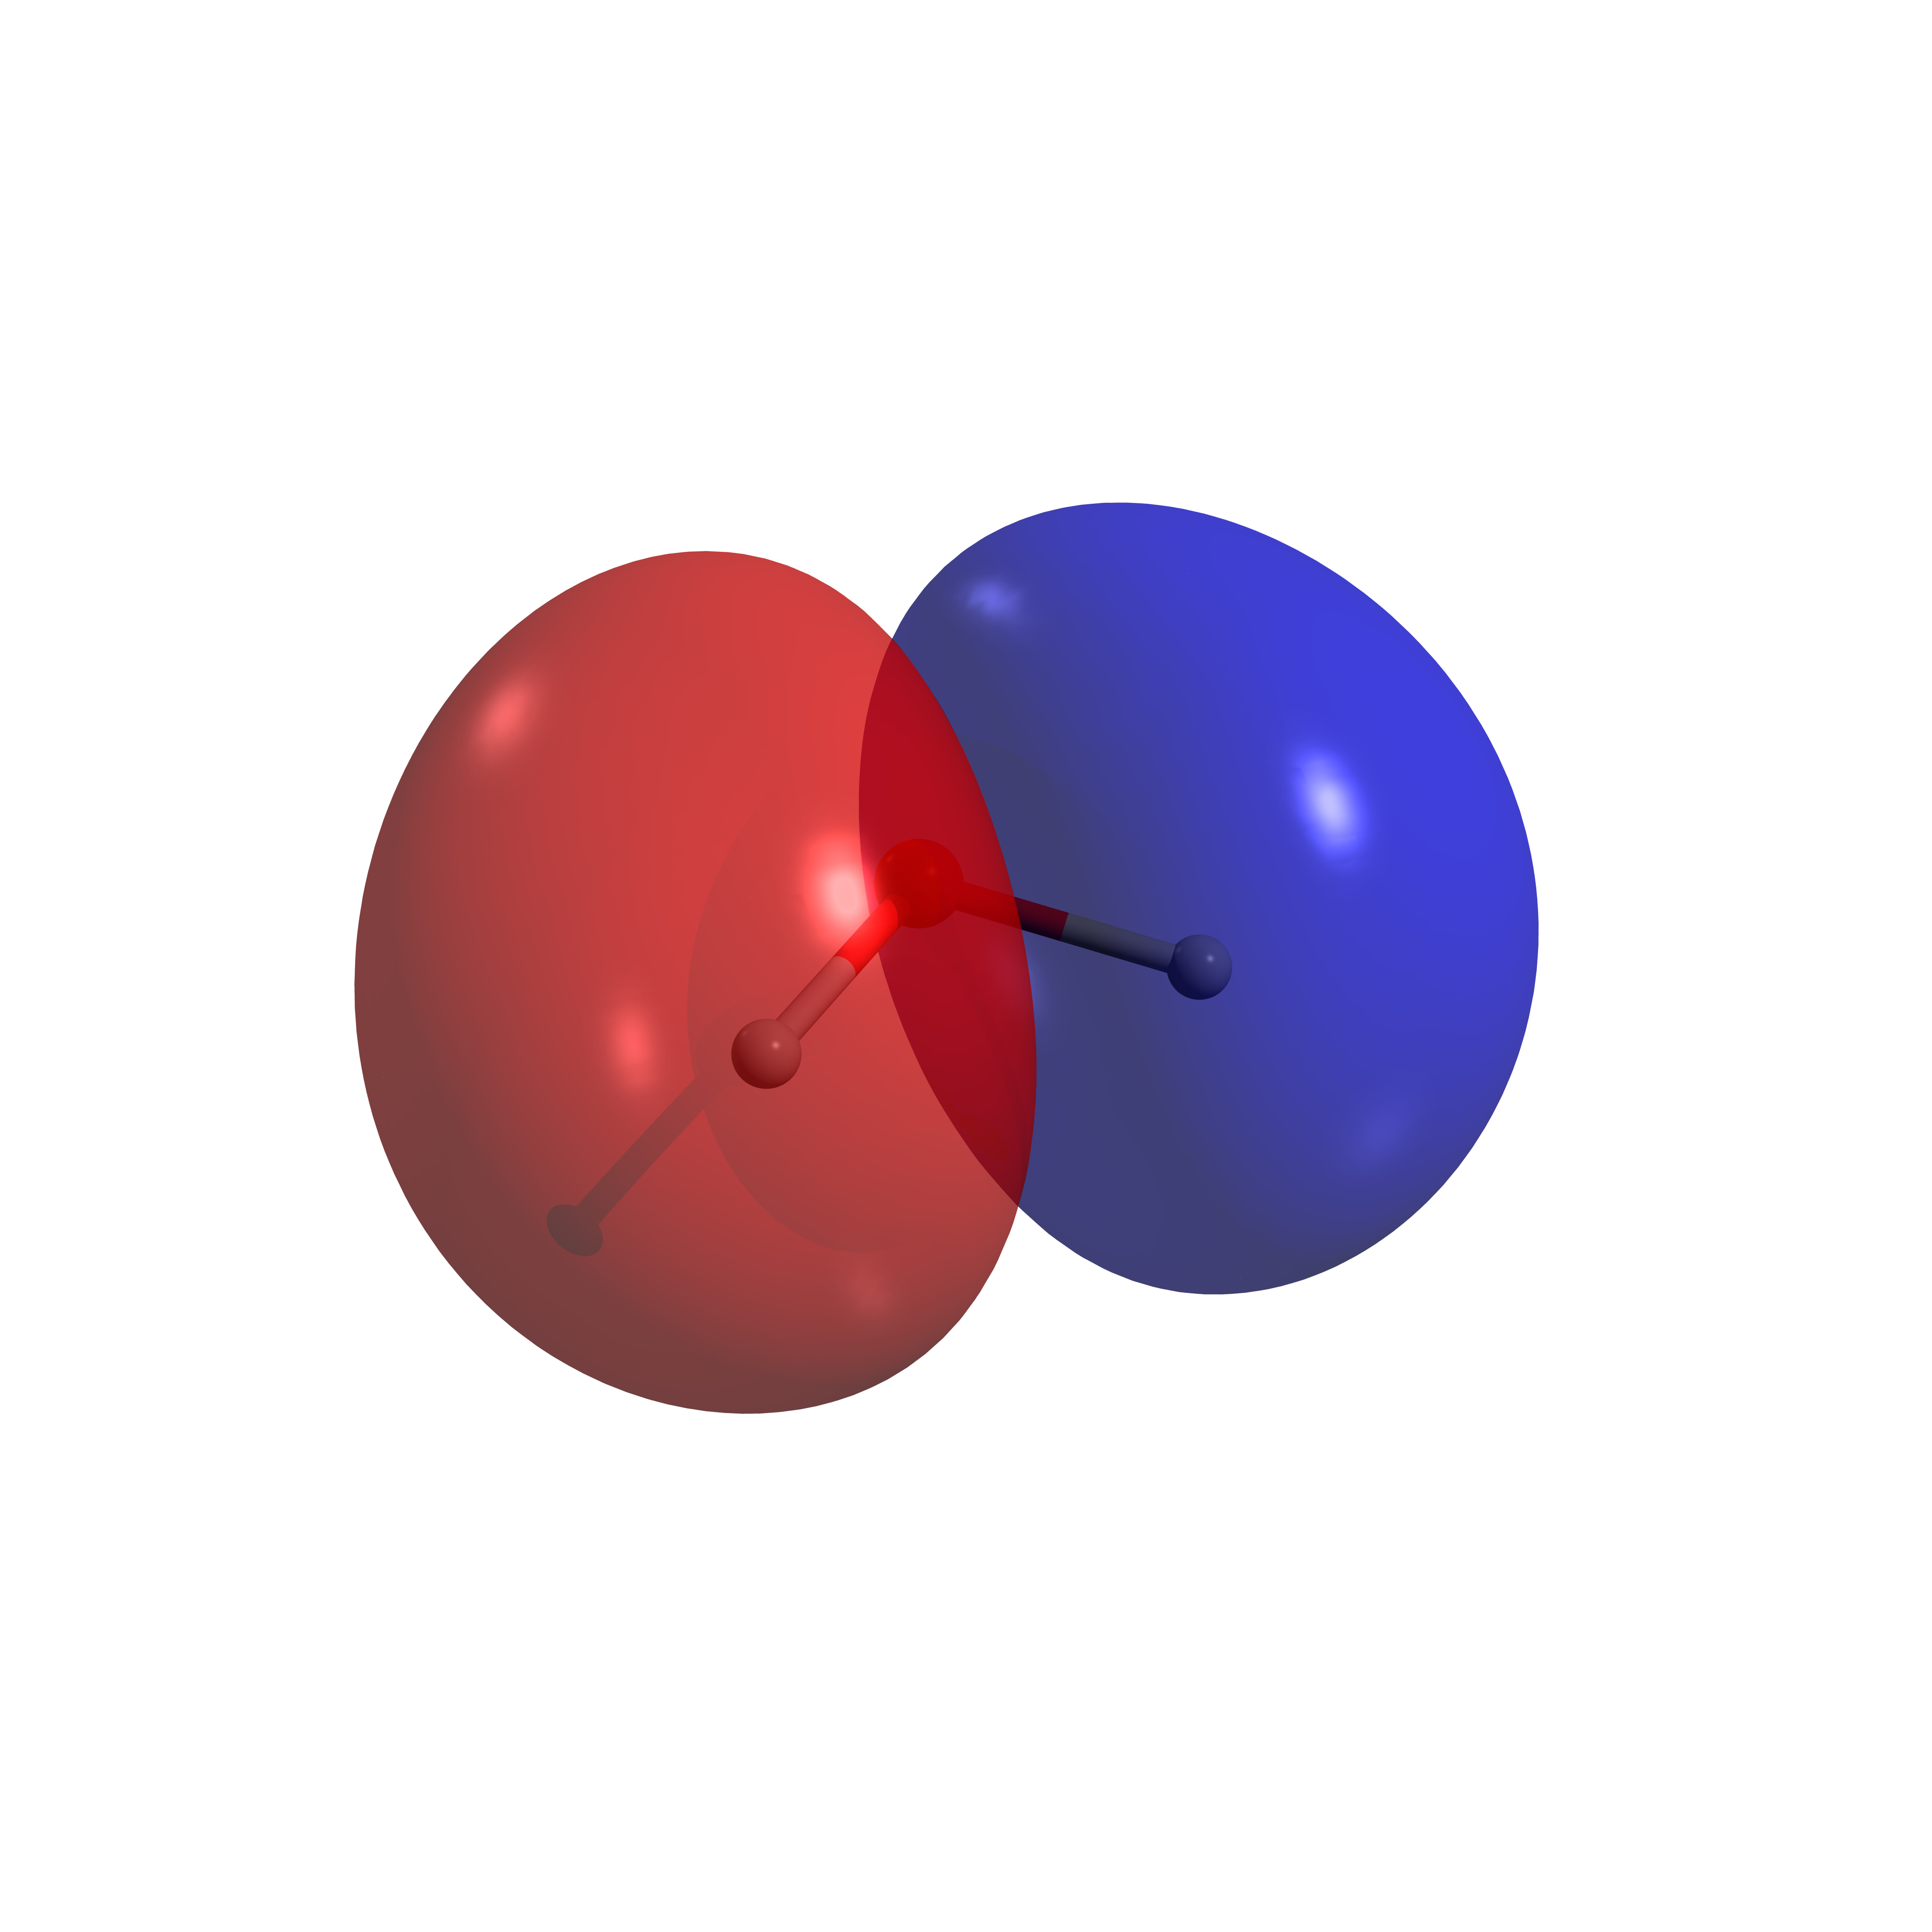
\includegraphics[trim=700 800 700 600, clip, width=0.45\textwidth]{res/H2O/h2o_w2.png}
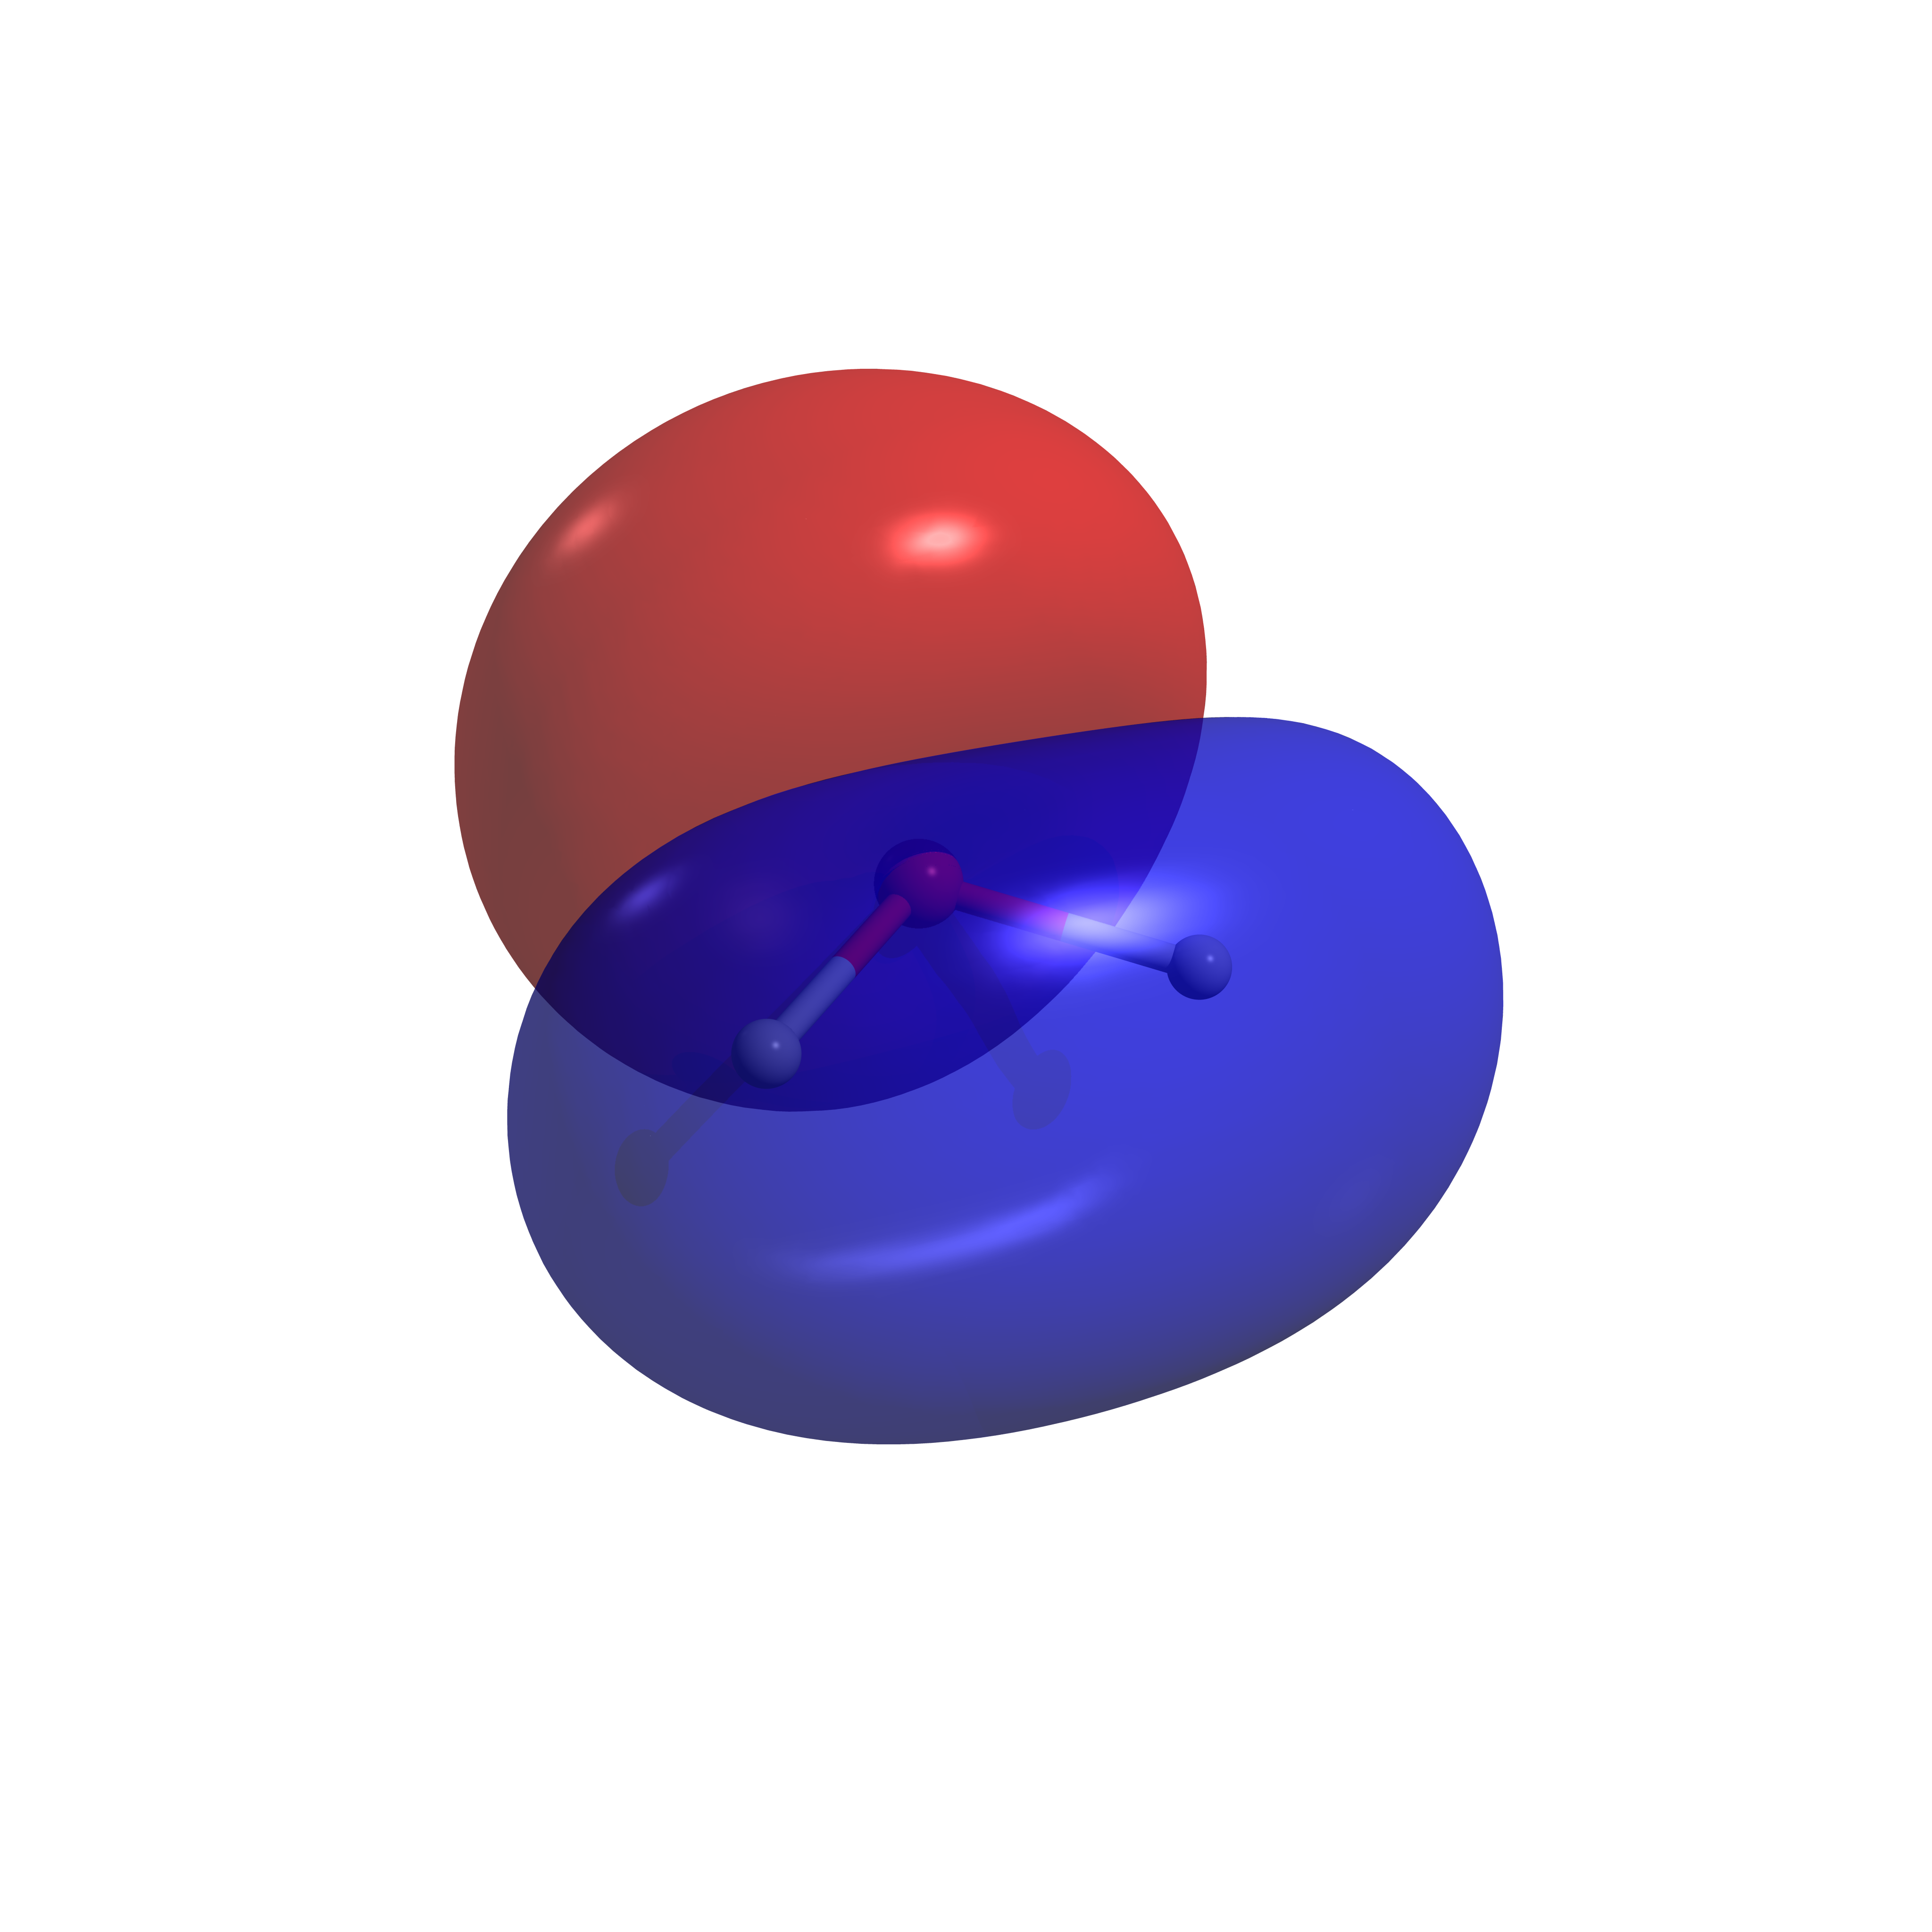
\includegraphics[trim=700 800 700 600, clip, width=0.45\textwidth]{res/H2O/h2o_w3.png}\\
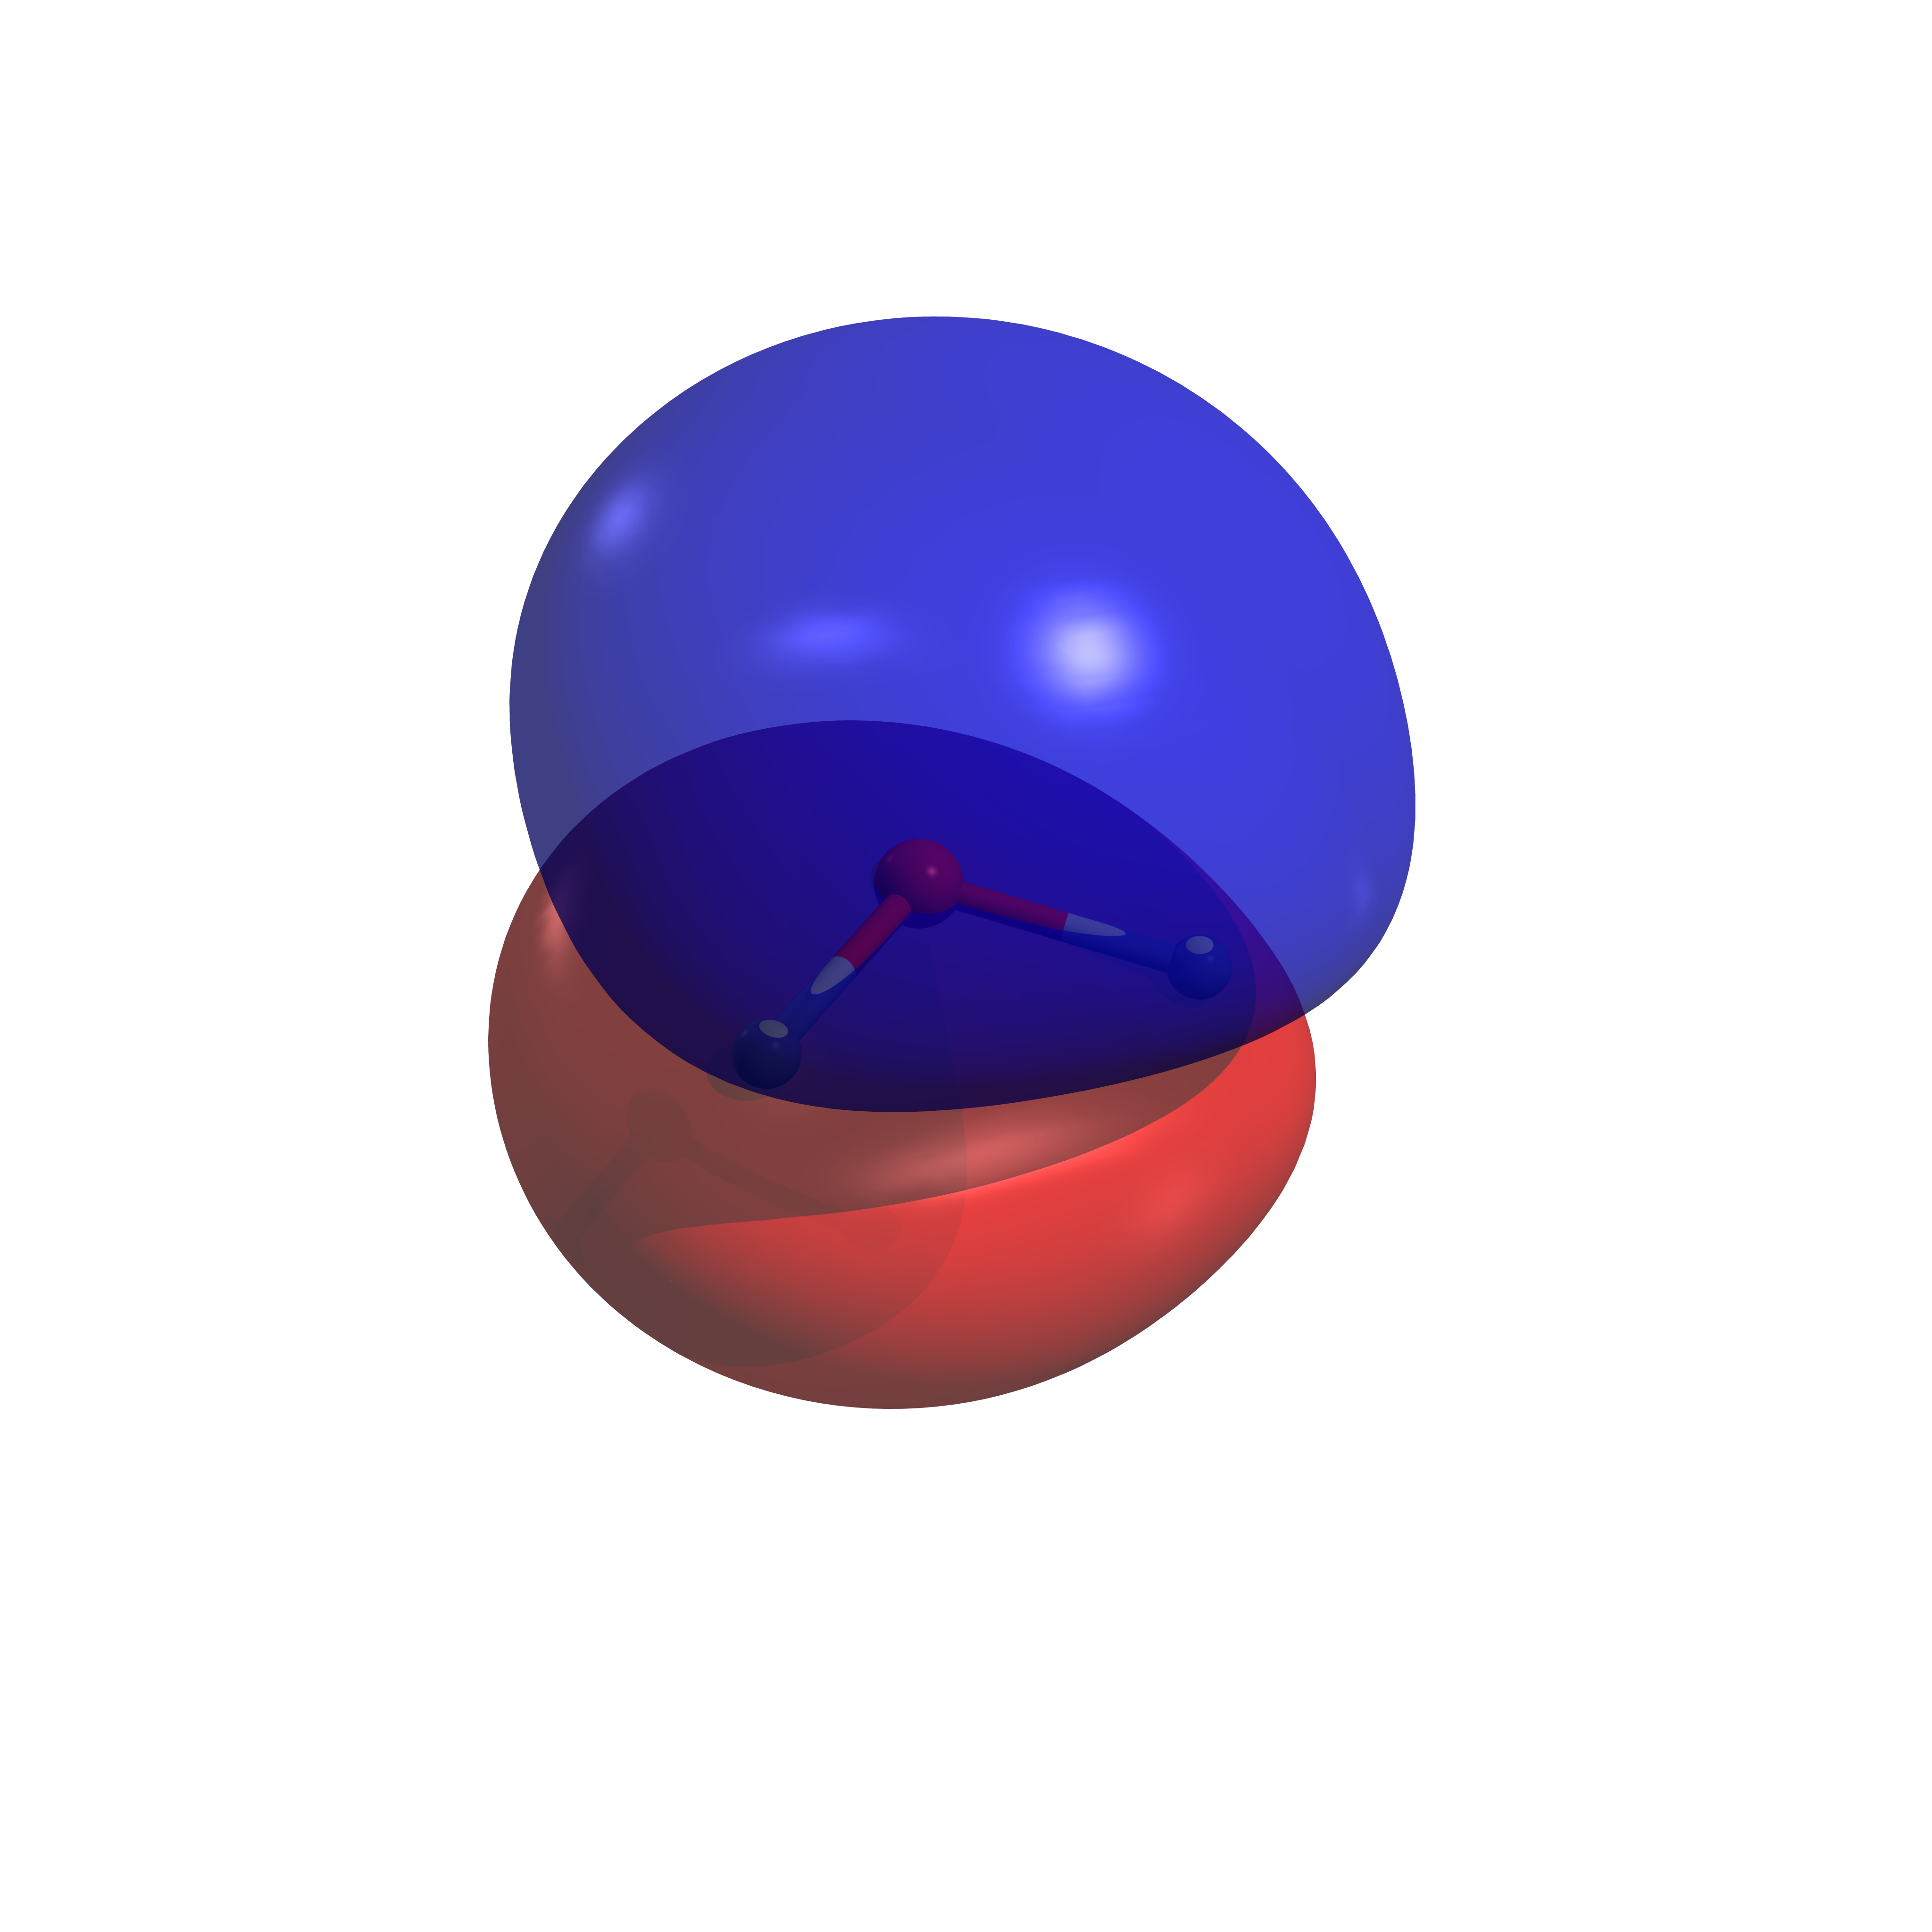
\includegraphics[trim=700 800 700 600, clip, width=0.45\textwidth]{res/H2O/h2o_w4.png}
\caption{Die fünf besetzten Orbitale des H$_2$O\-/Moleküls,
nach aufsteigender Energie sortiert.
\textcolor{blue}{$\blacksquare$} positiv,
\textcolor{red}{$\blacksquare$} negativ.}\label{h2o_orbitals}
\end{figure}

\newpage
\item Ammoniak (NH$_3$):
\begin{figure}[H]
\centering
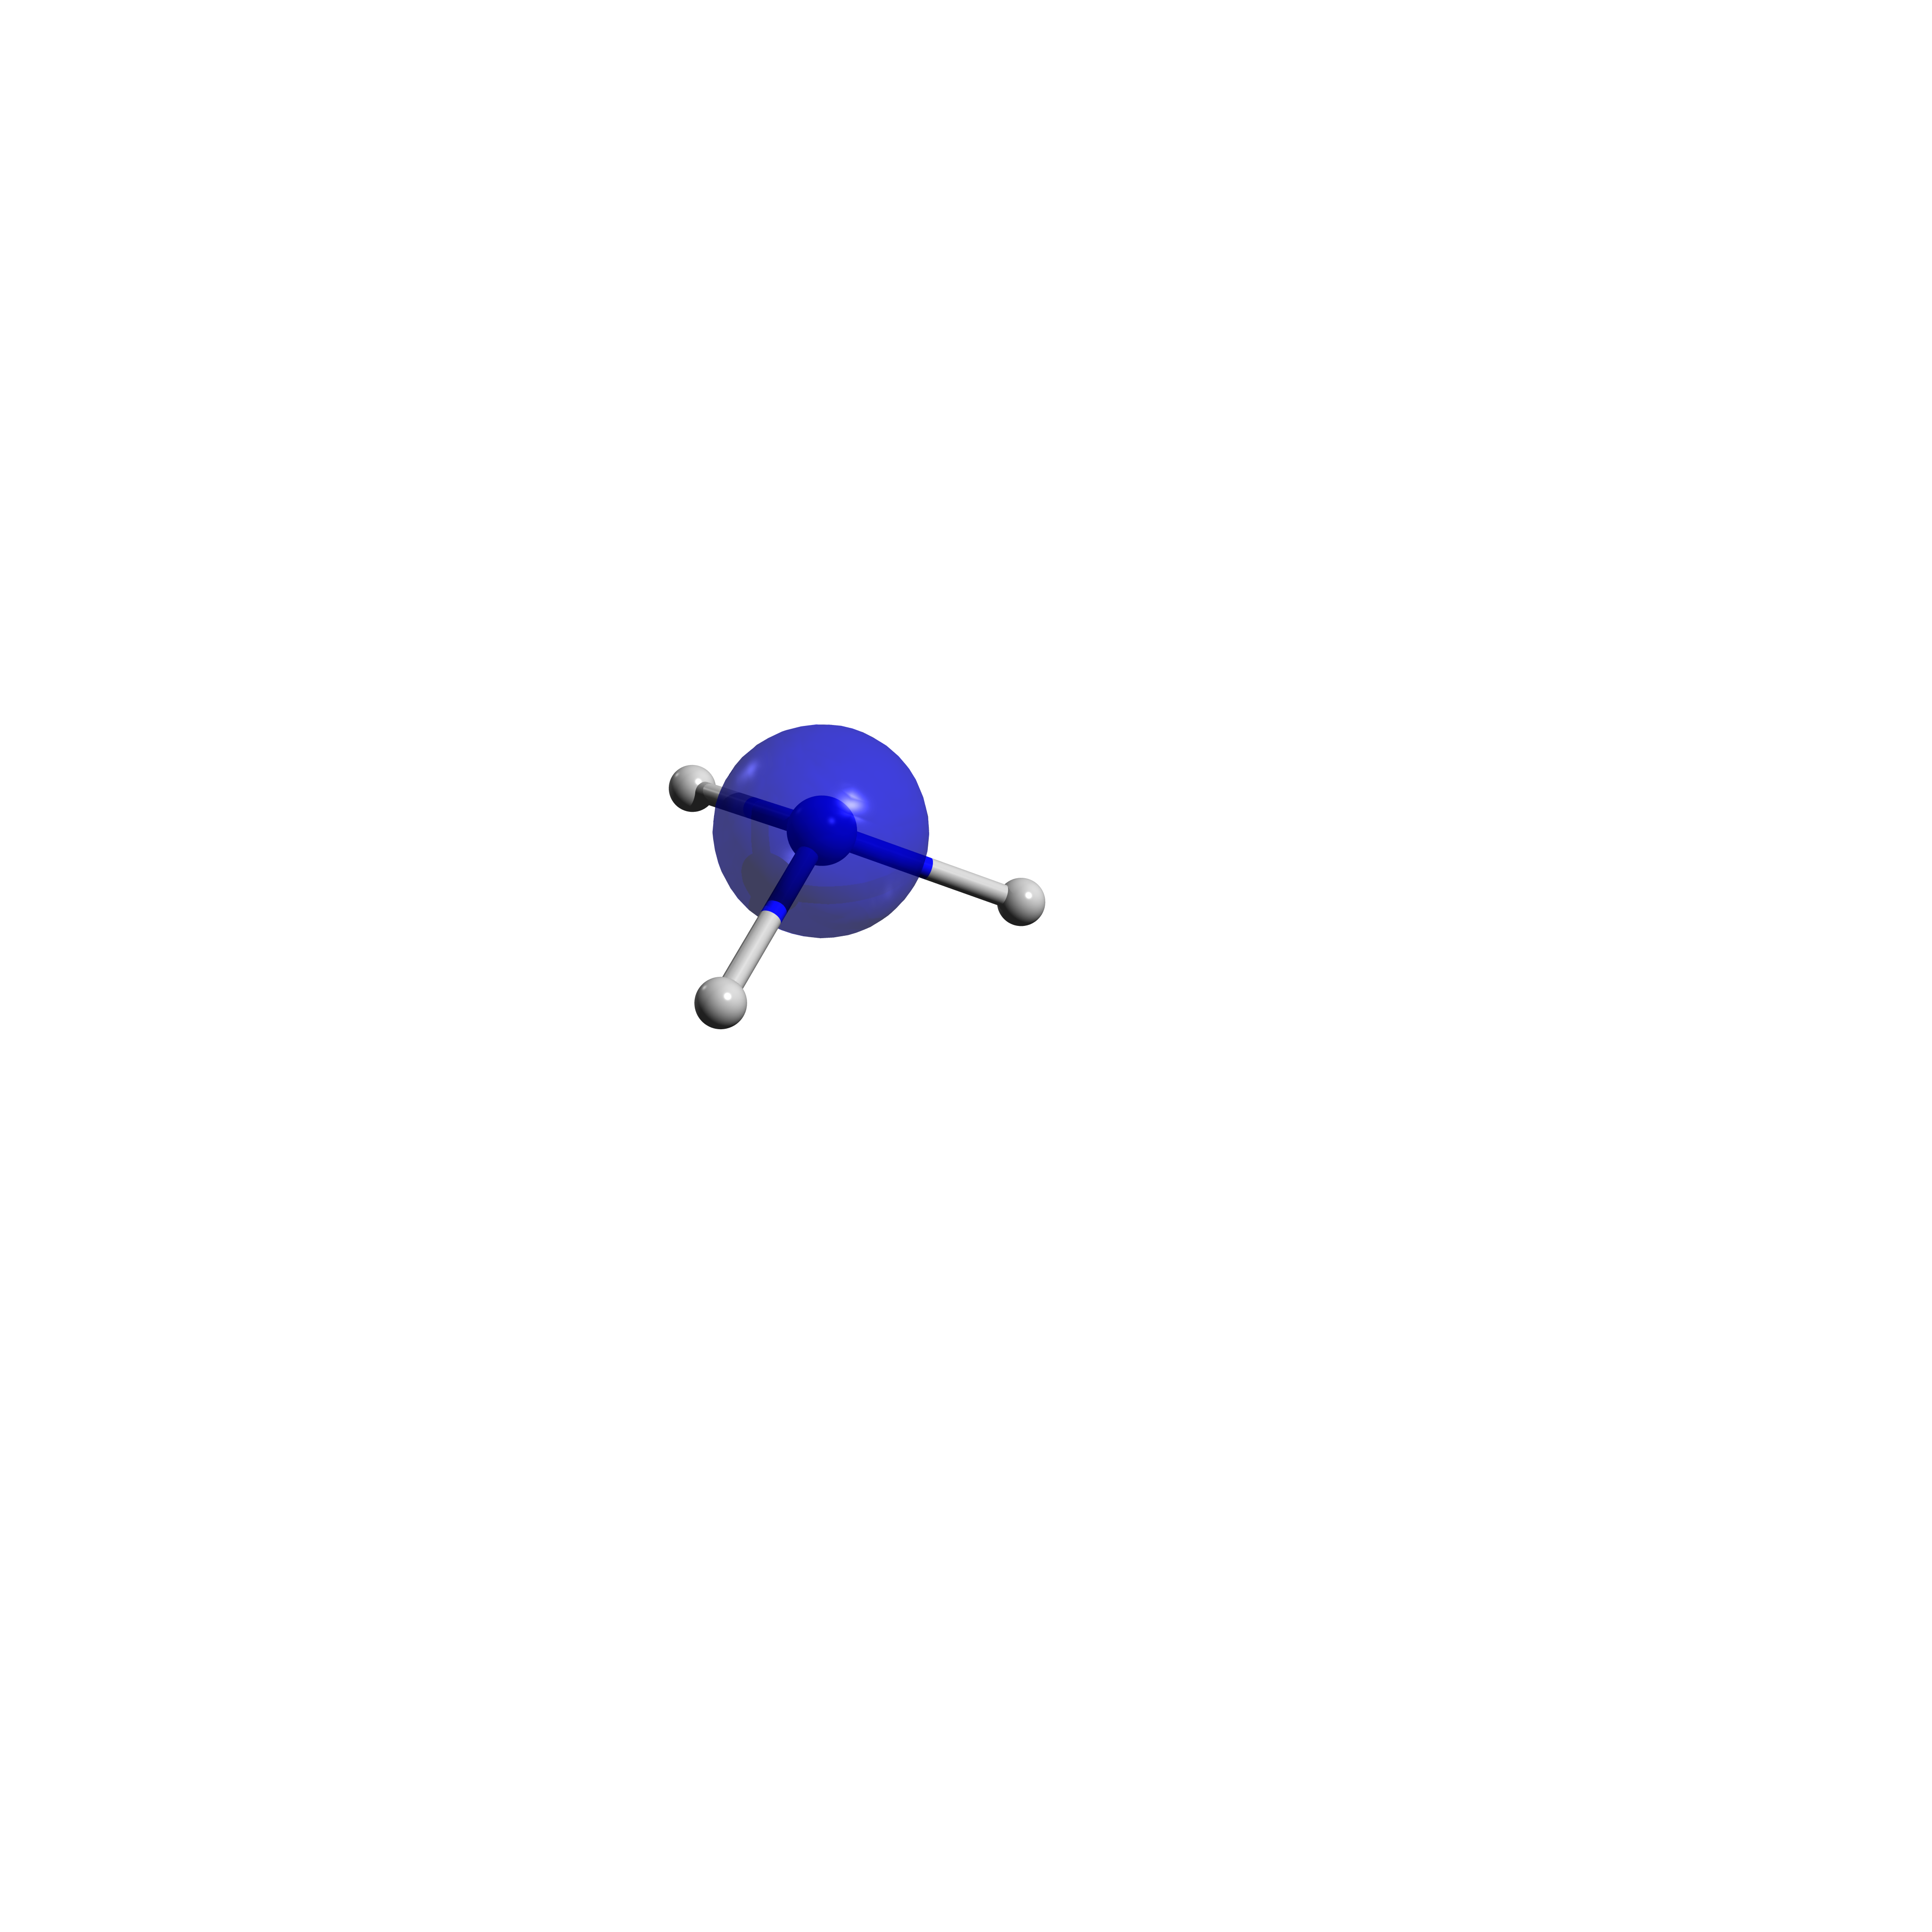
\includegraphics[trim=700 1200 1200 700, clip, width=0.45\textwidth]{res/NH3/nh3_w0.png}
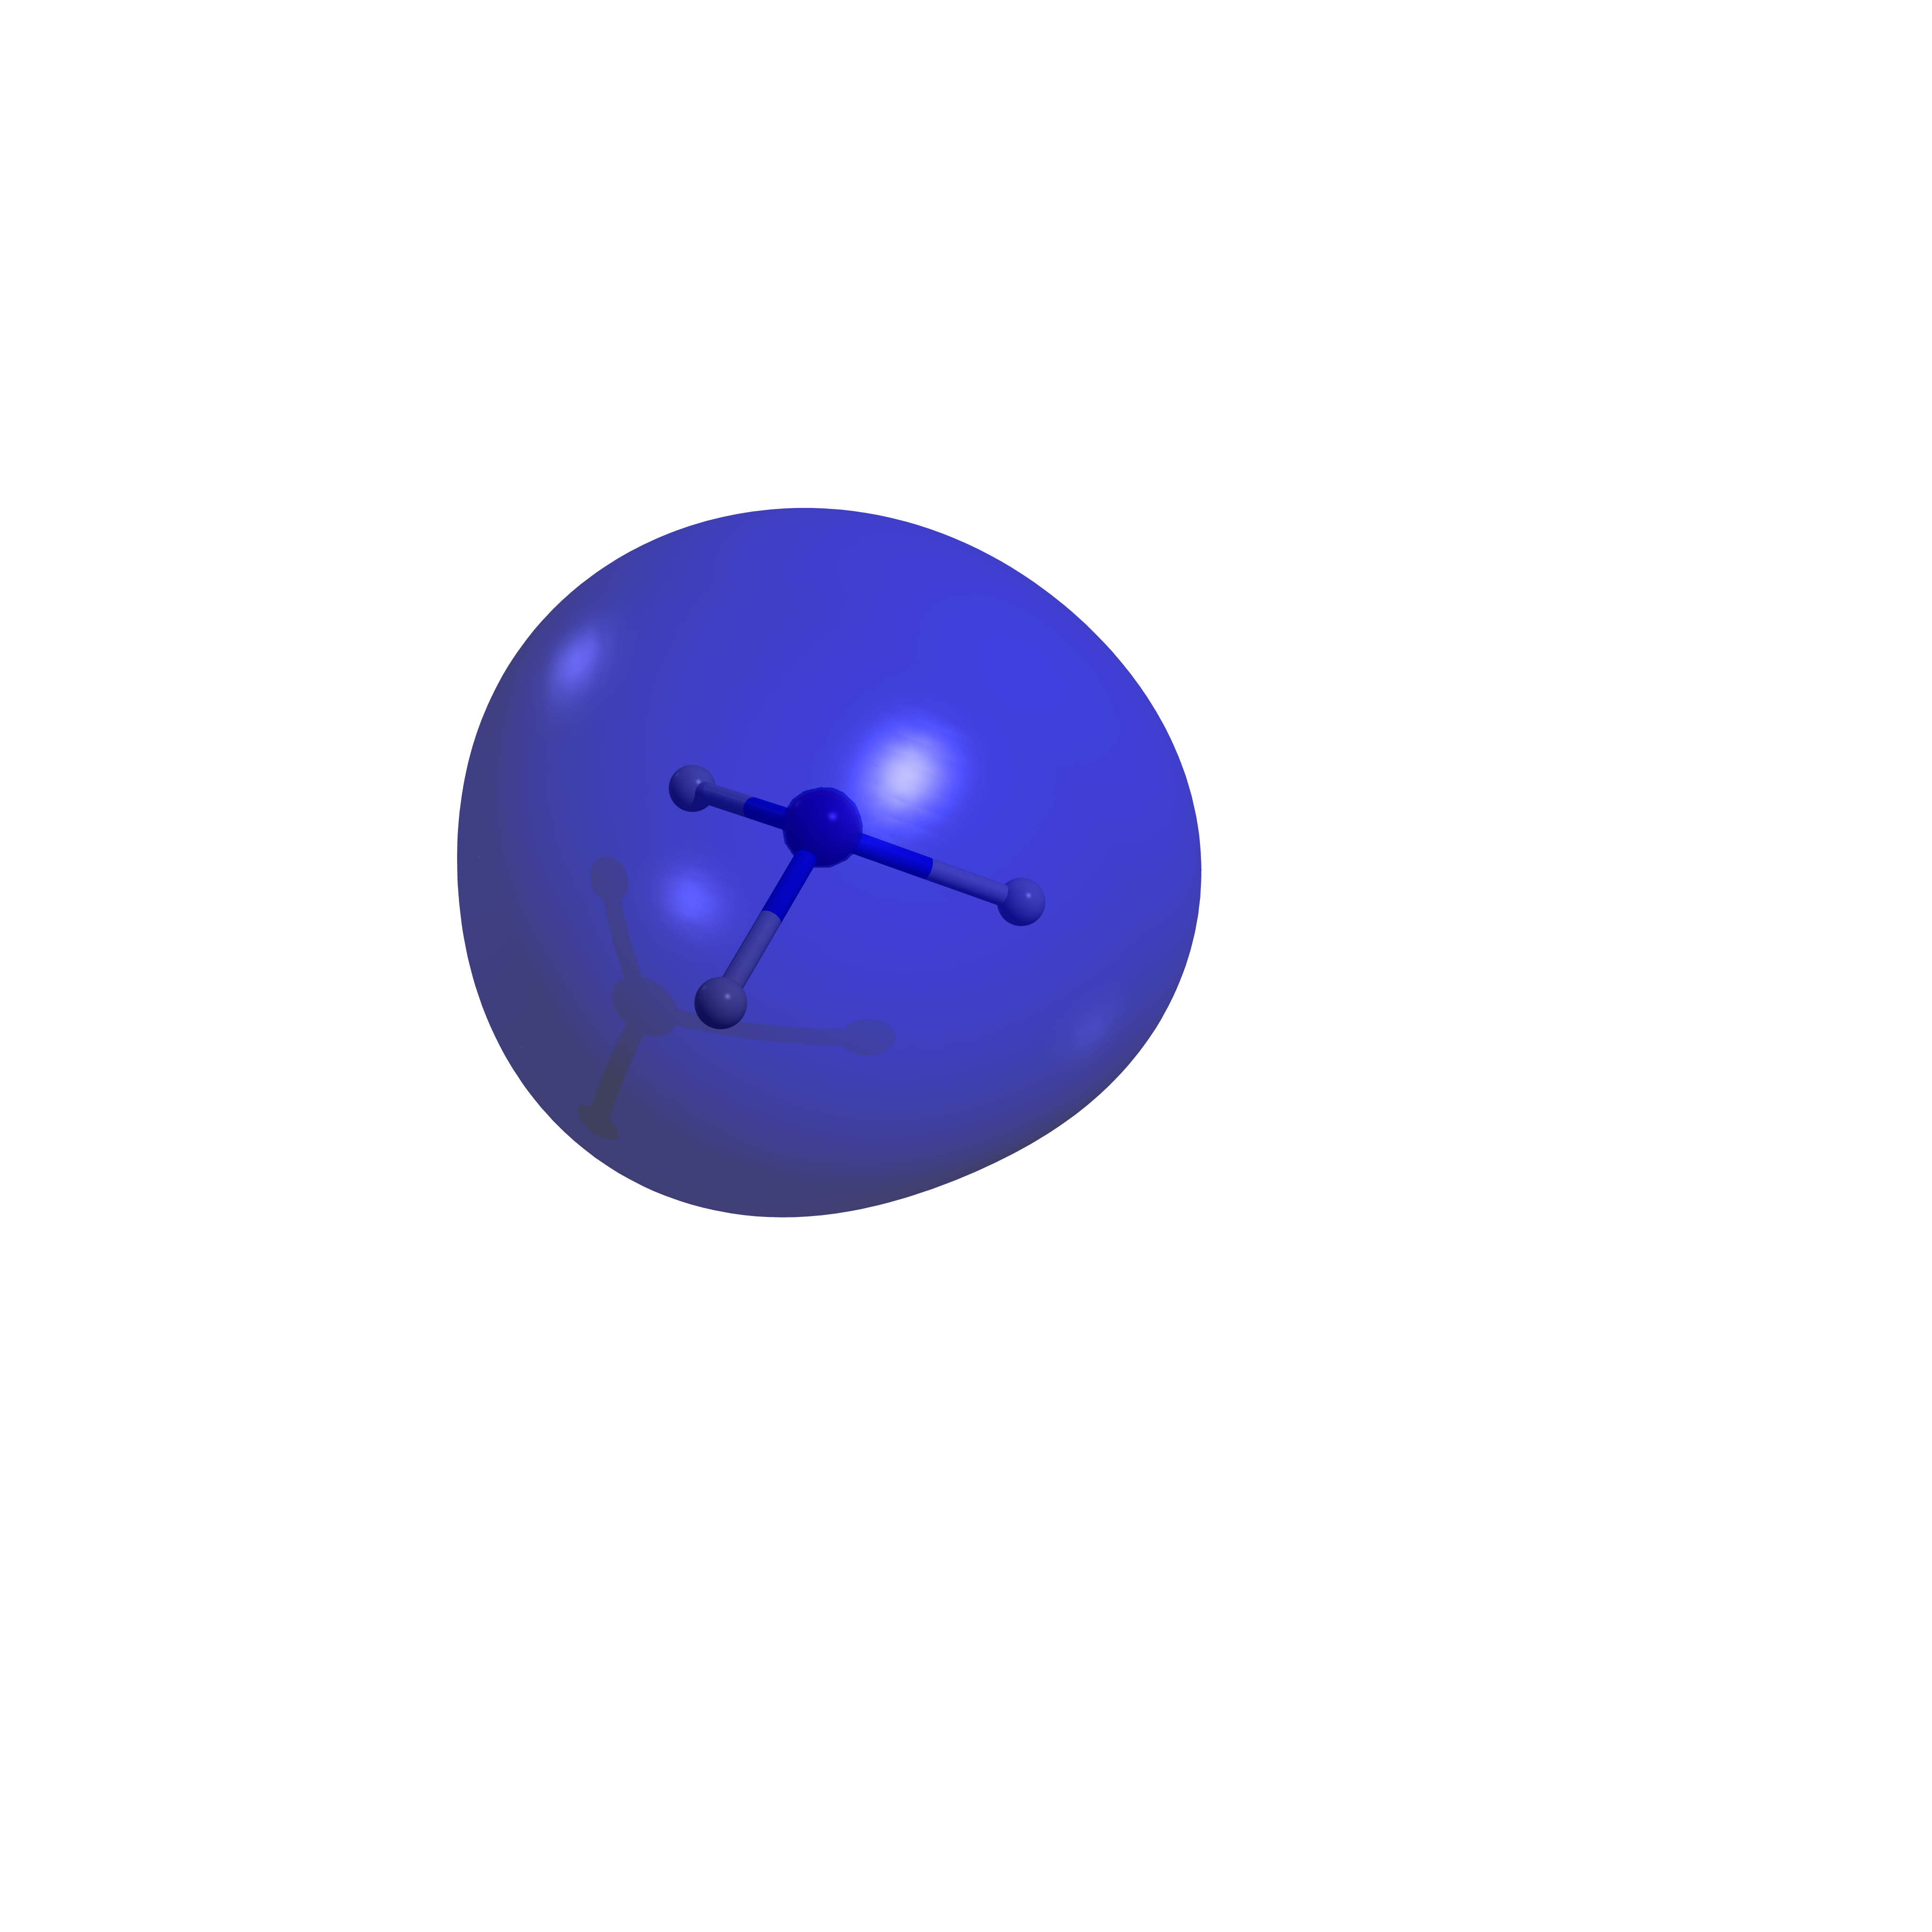
\includegraphics[trim=700 1200 1200 700, clip, width=0.45\textwidth]{res/NH3/nh3_w1.png}\\
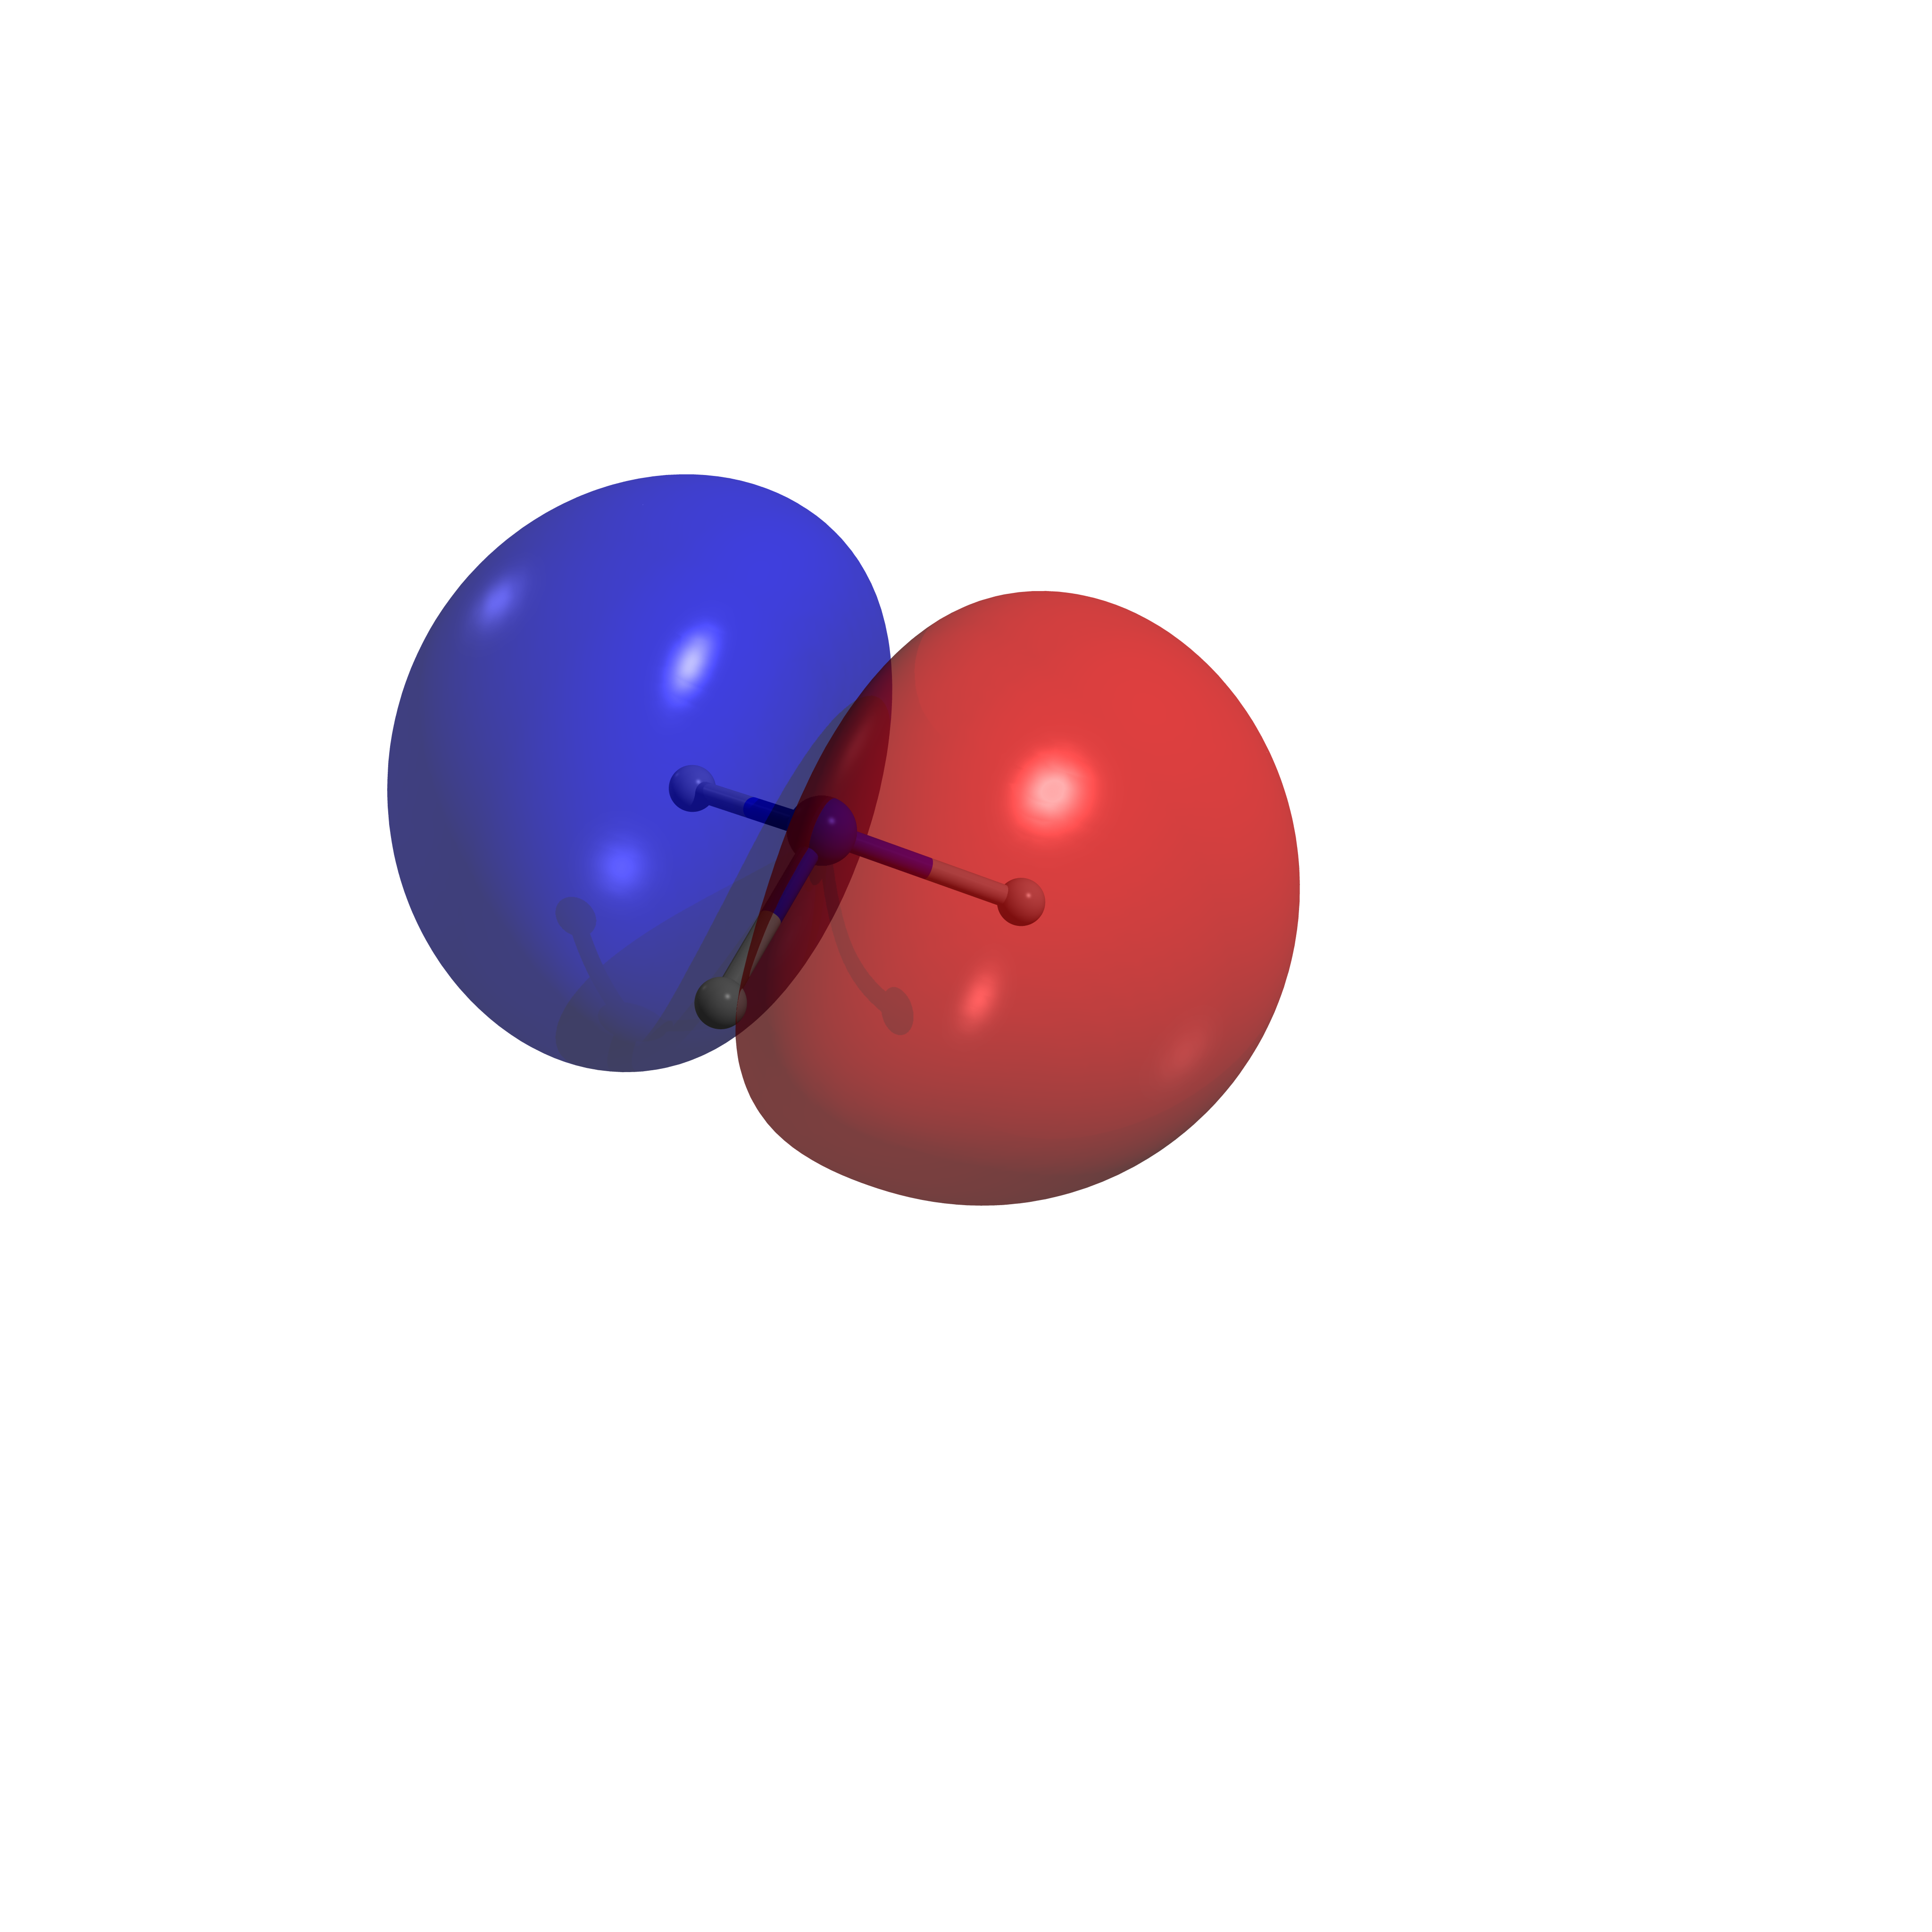
\includegraphics[trim=700 1200 1200 700, clip, width=0.45\textwidth]{res/NH3/nh3_w2.png}
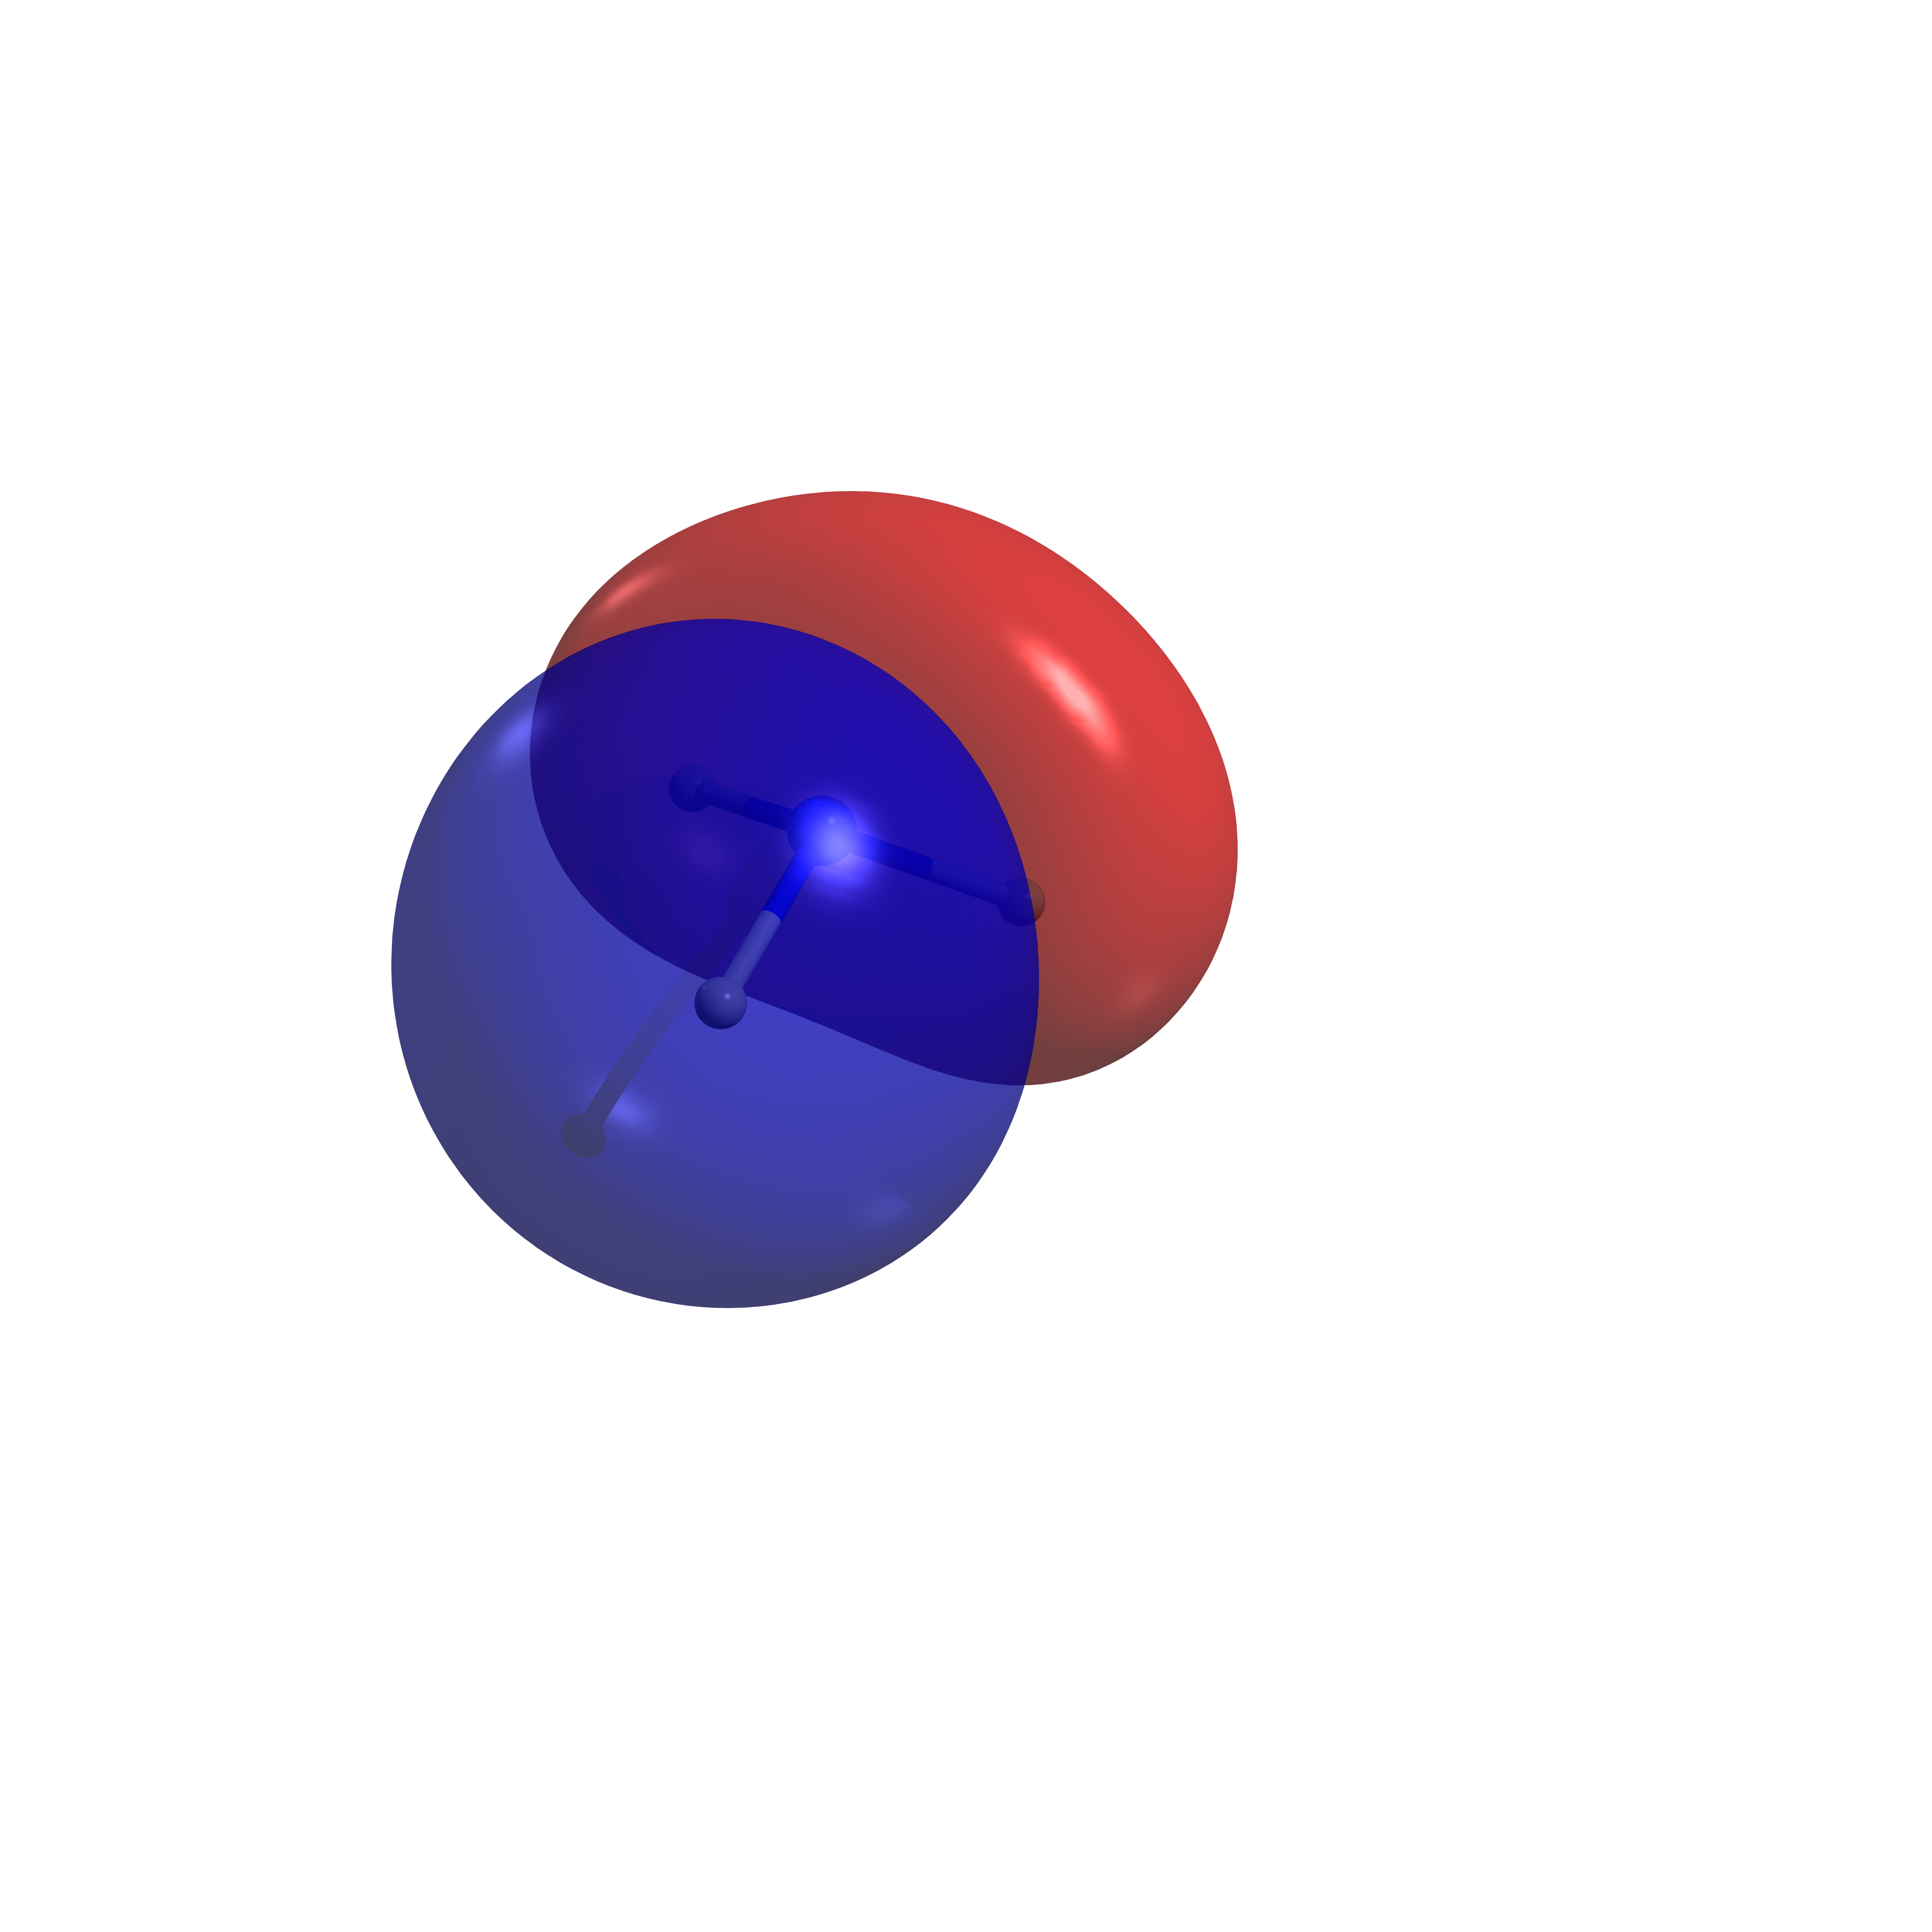
\includegraphics[trim=700 1200 1200 700, clip, width=0.45\textwidth]{res/NH3/nh3_w3.png}\\
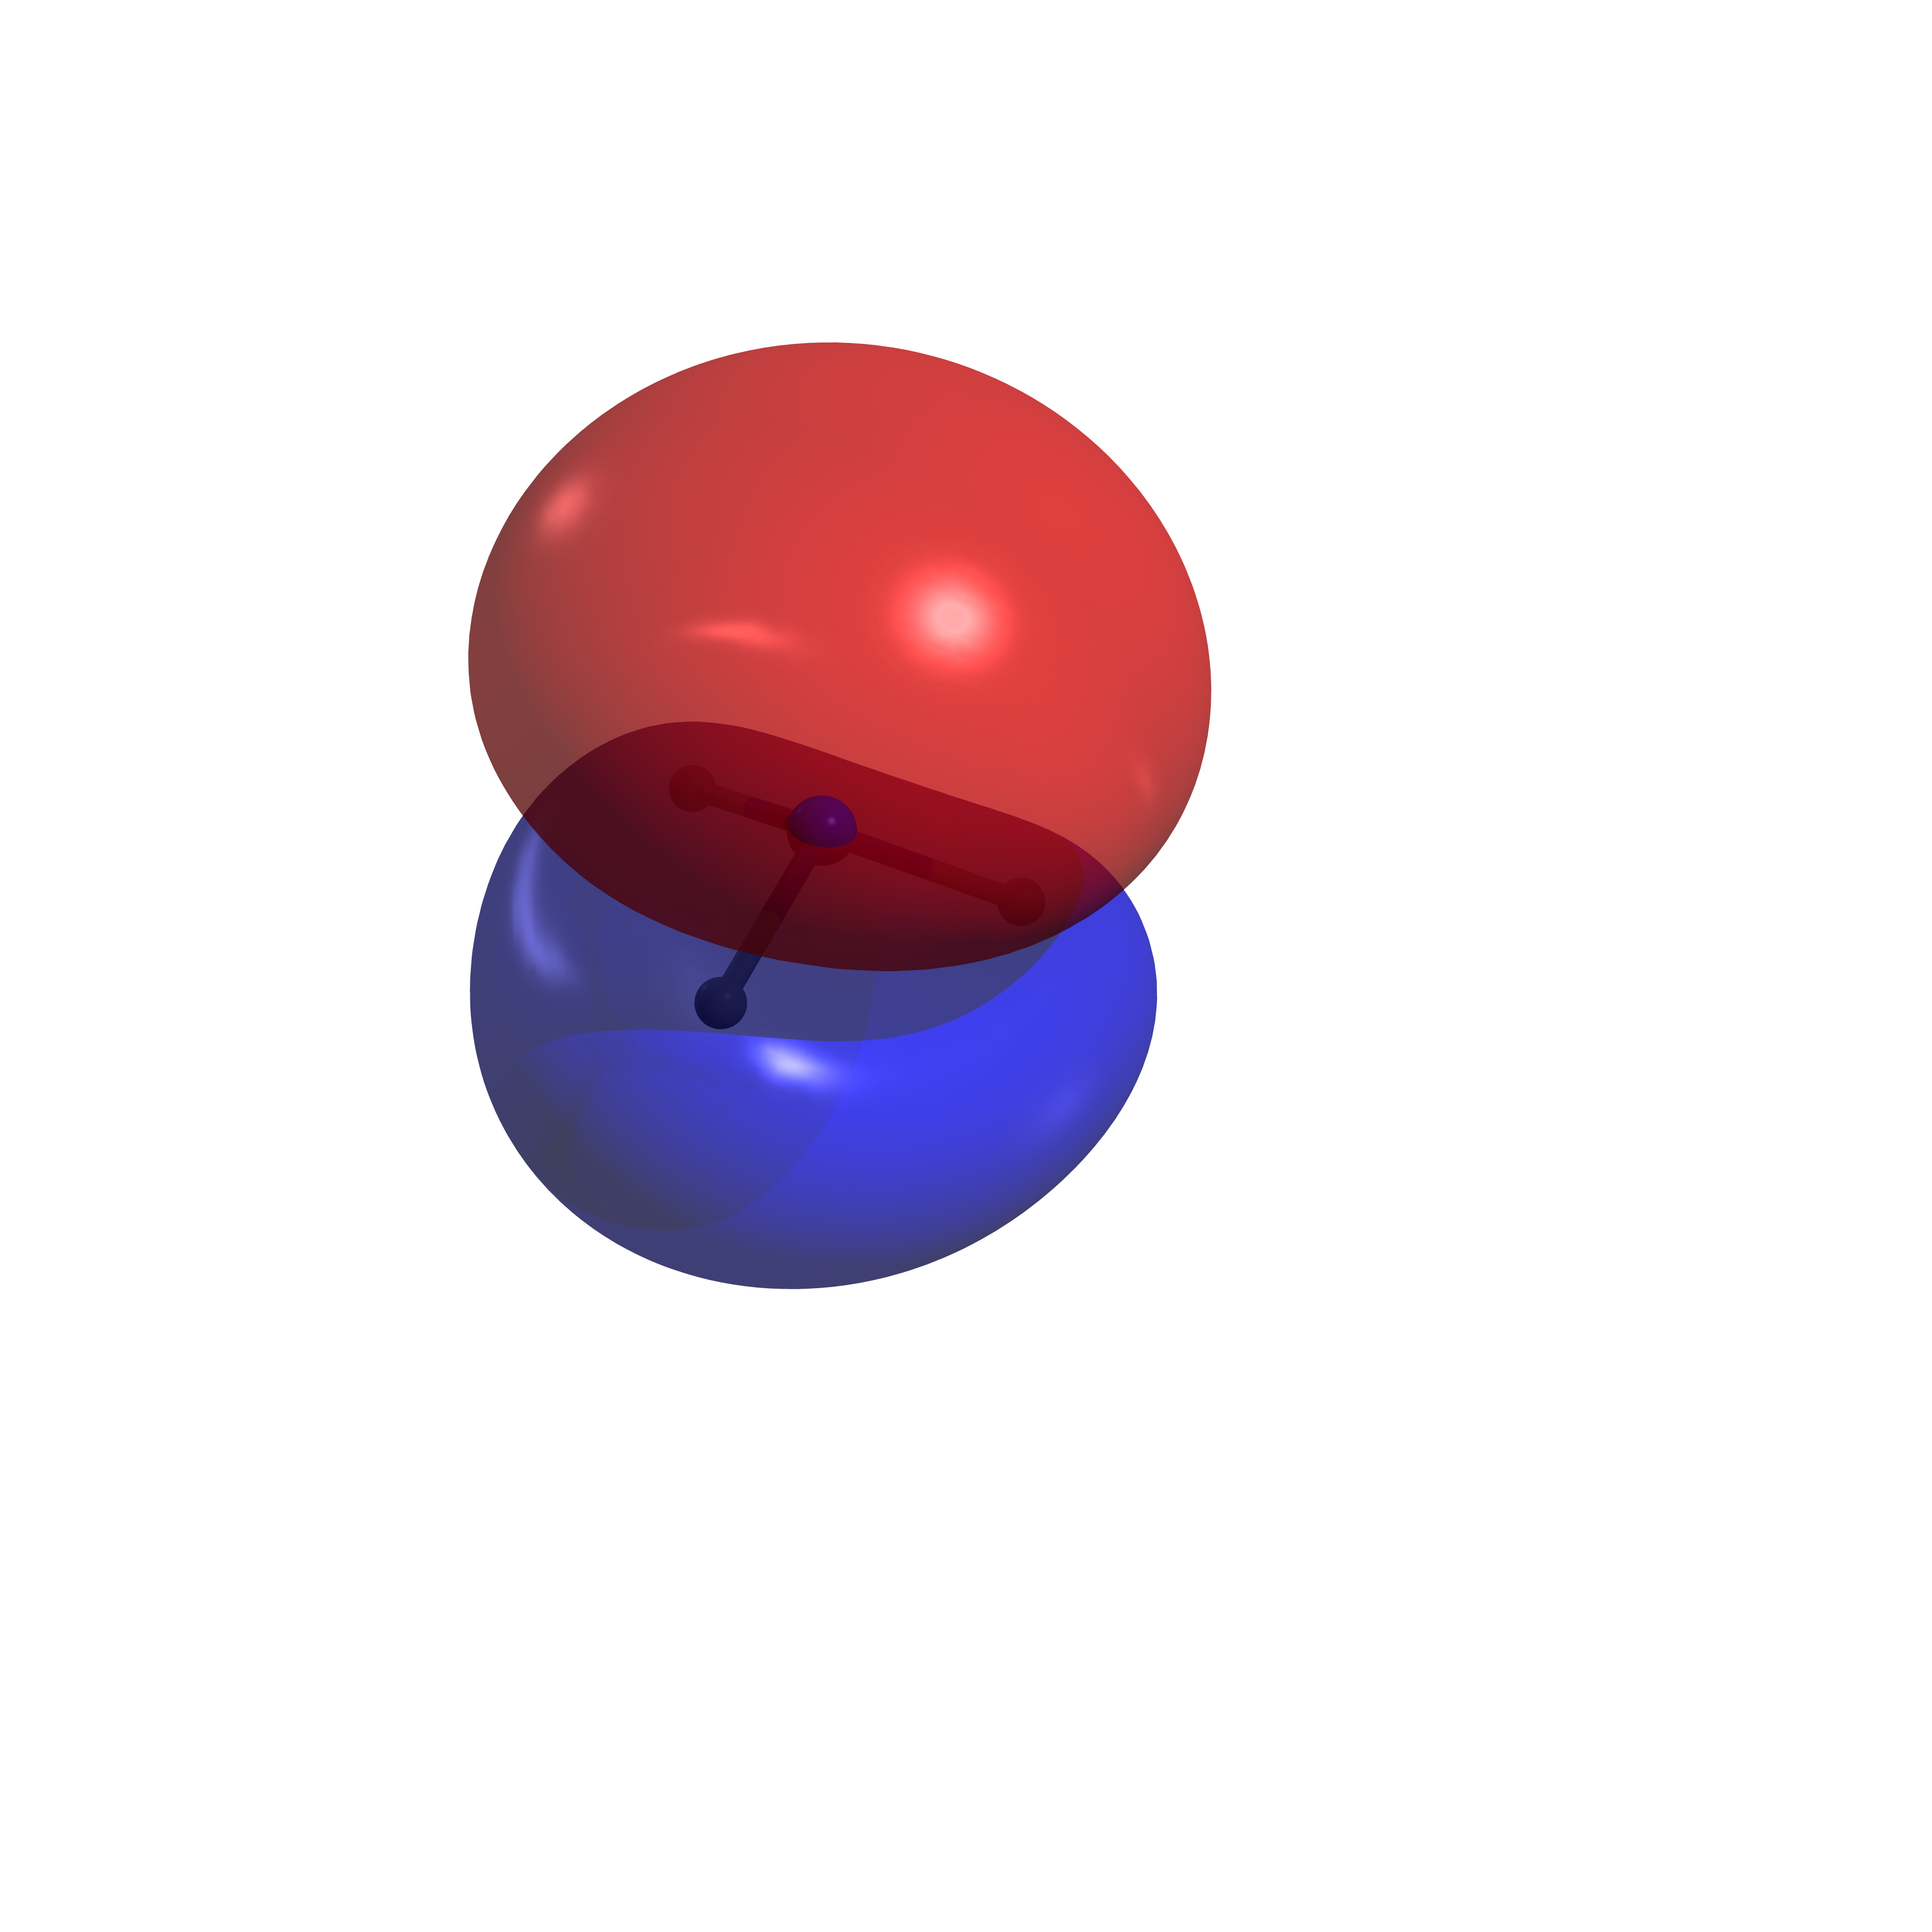
\includegraphics[trim=700 1200 1200 700, clip, width=0.45\textwidth]{res/NH3/nh3_w4.png}
\caption{Die fünf besetzten Orbitale des NH$_3$\-/Moleküls,
nach aufsteigender Energie sortiert.
\textcolor{blue}{$\blacksquare$} positiv,
\textcolor{red}{$\blacksquare$} negativ.}\label{nh3_orbitals}
\end{figure}

\newpage
\item Methan (CH$_4$):
\begin{figure}[H]
\centering
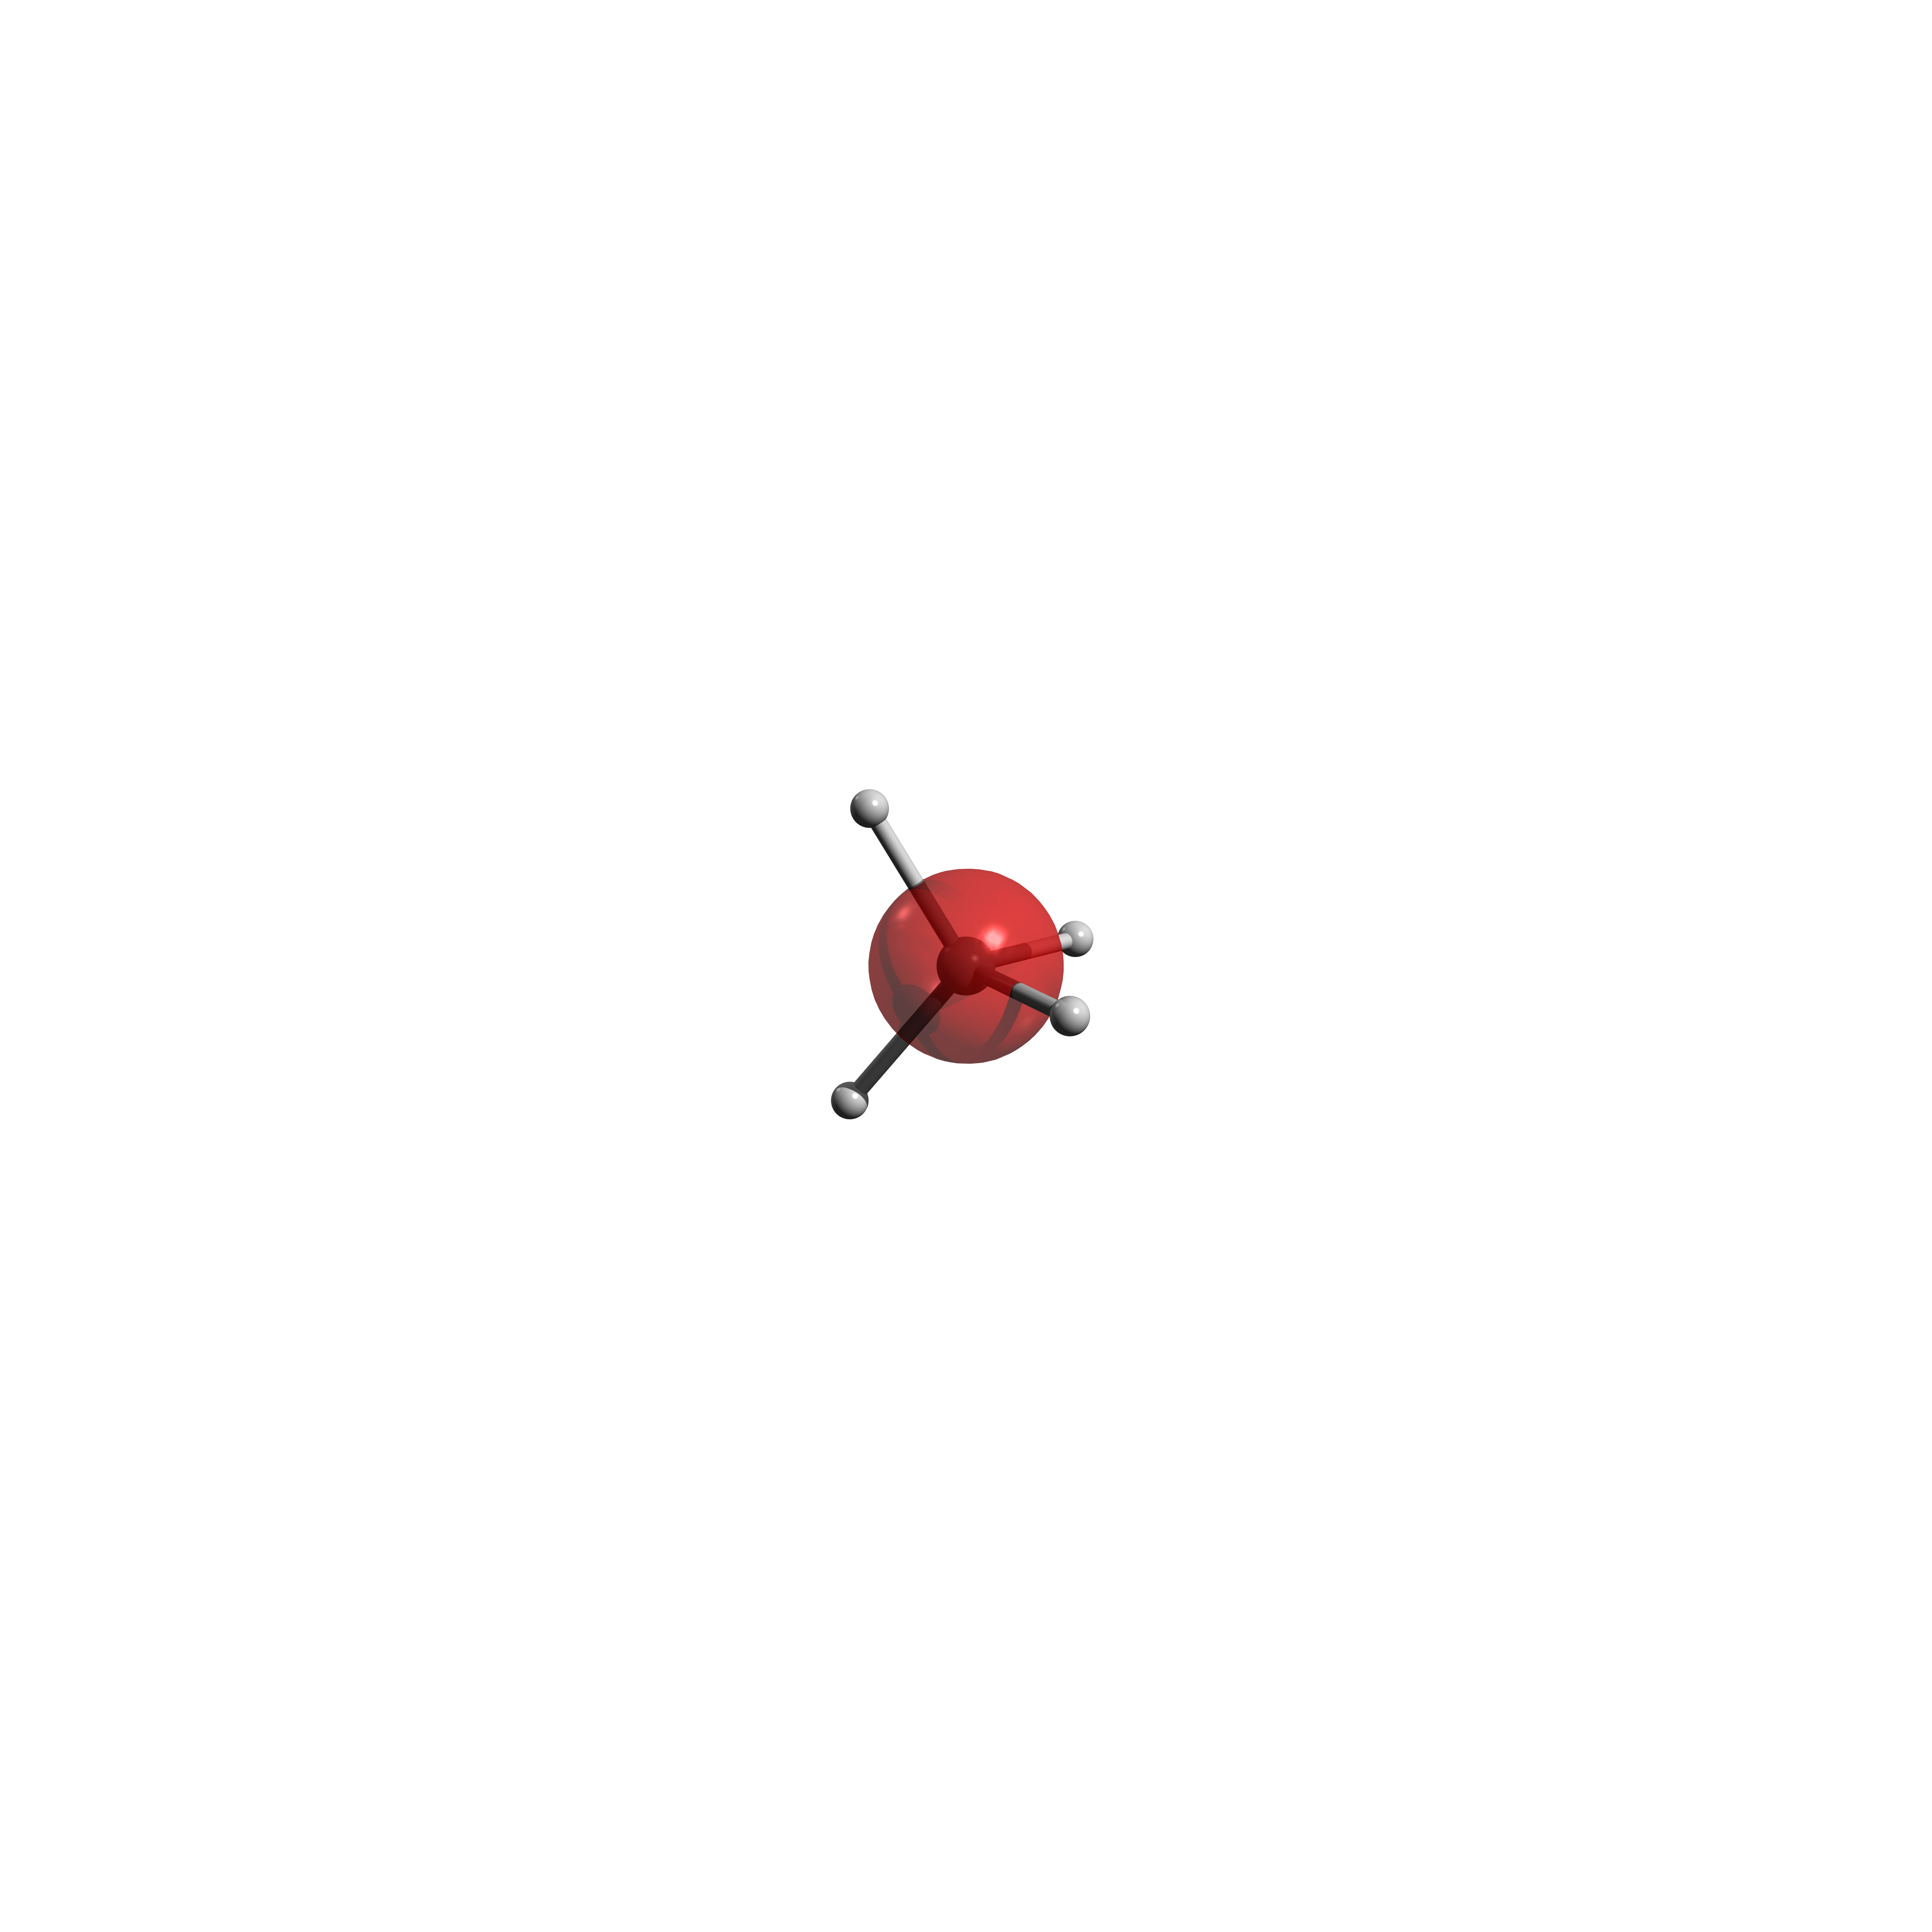
\includegraphics[trim=1200 1200 1200 1200, clip, width=0.45\textwidth]{res/CH4/ch4_w0.png}
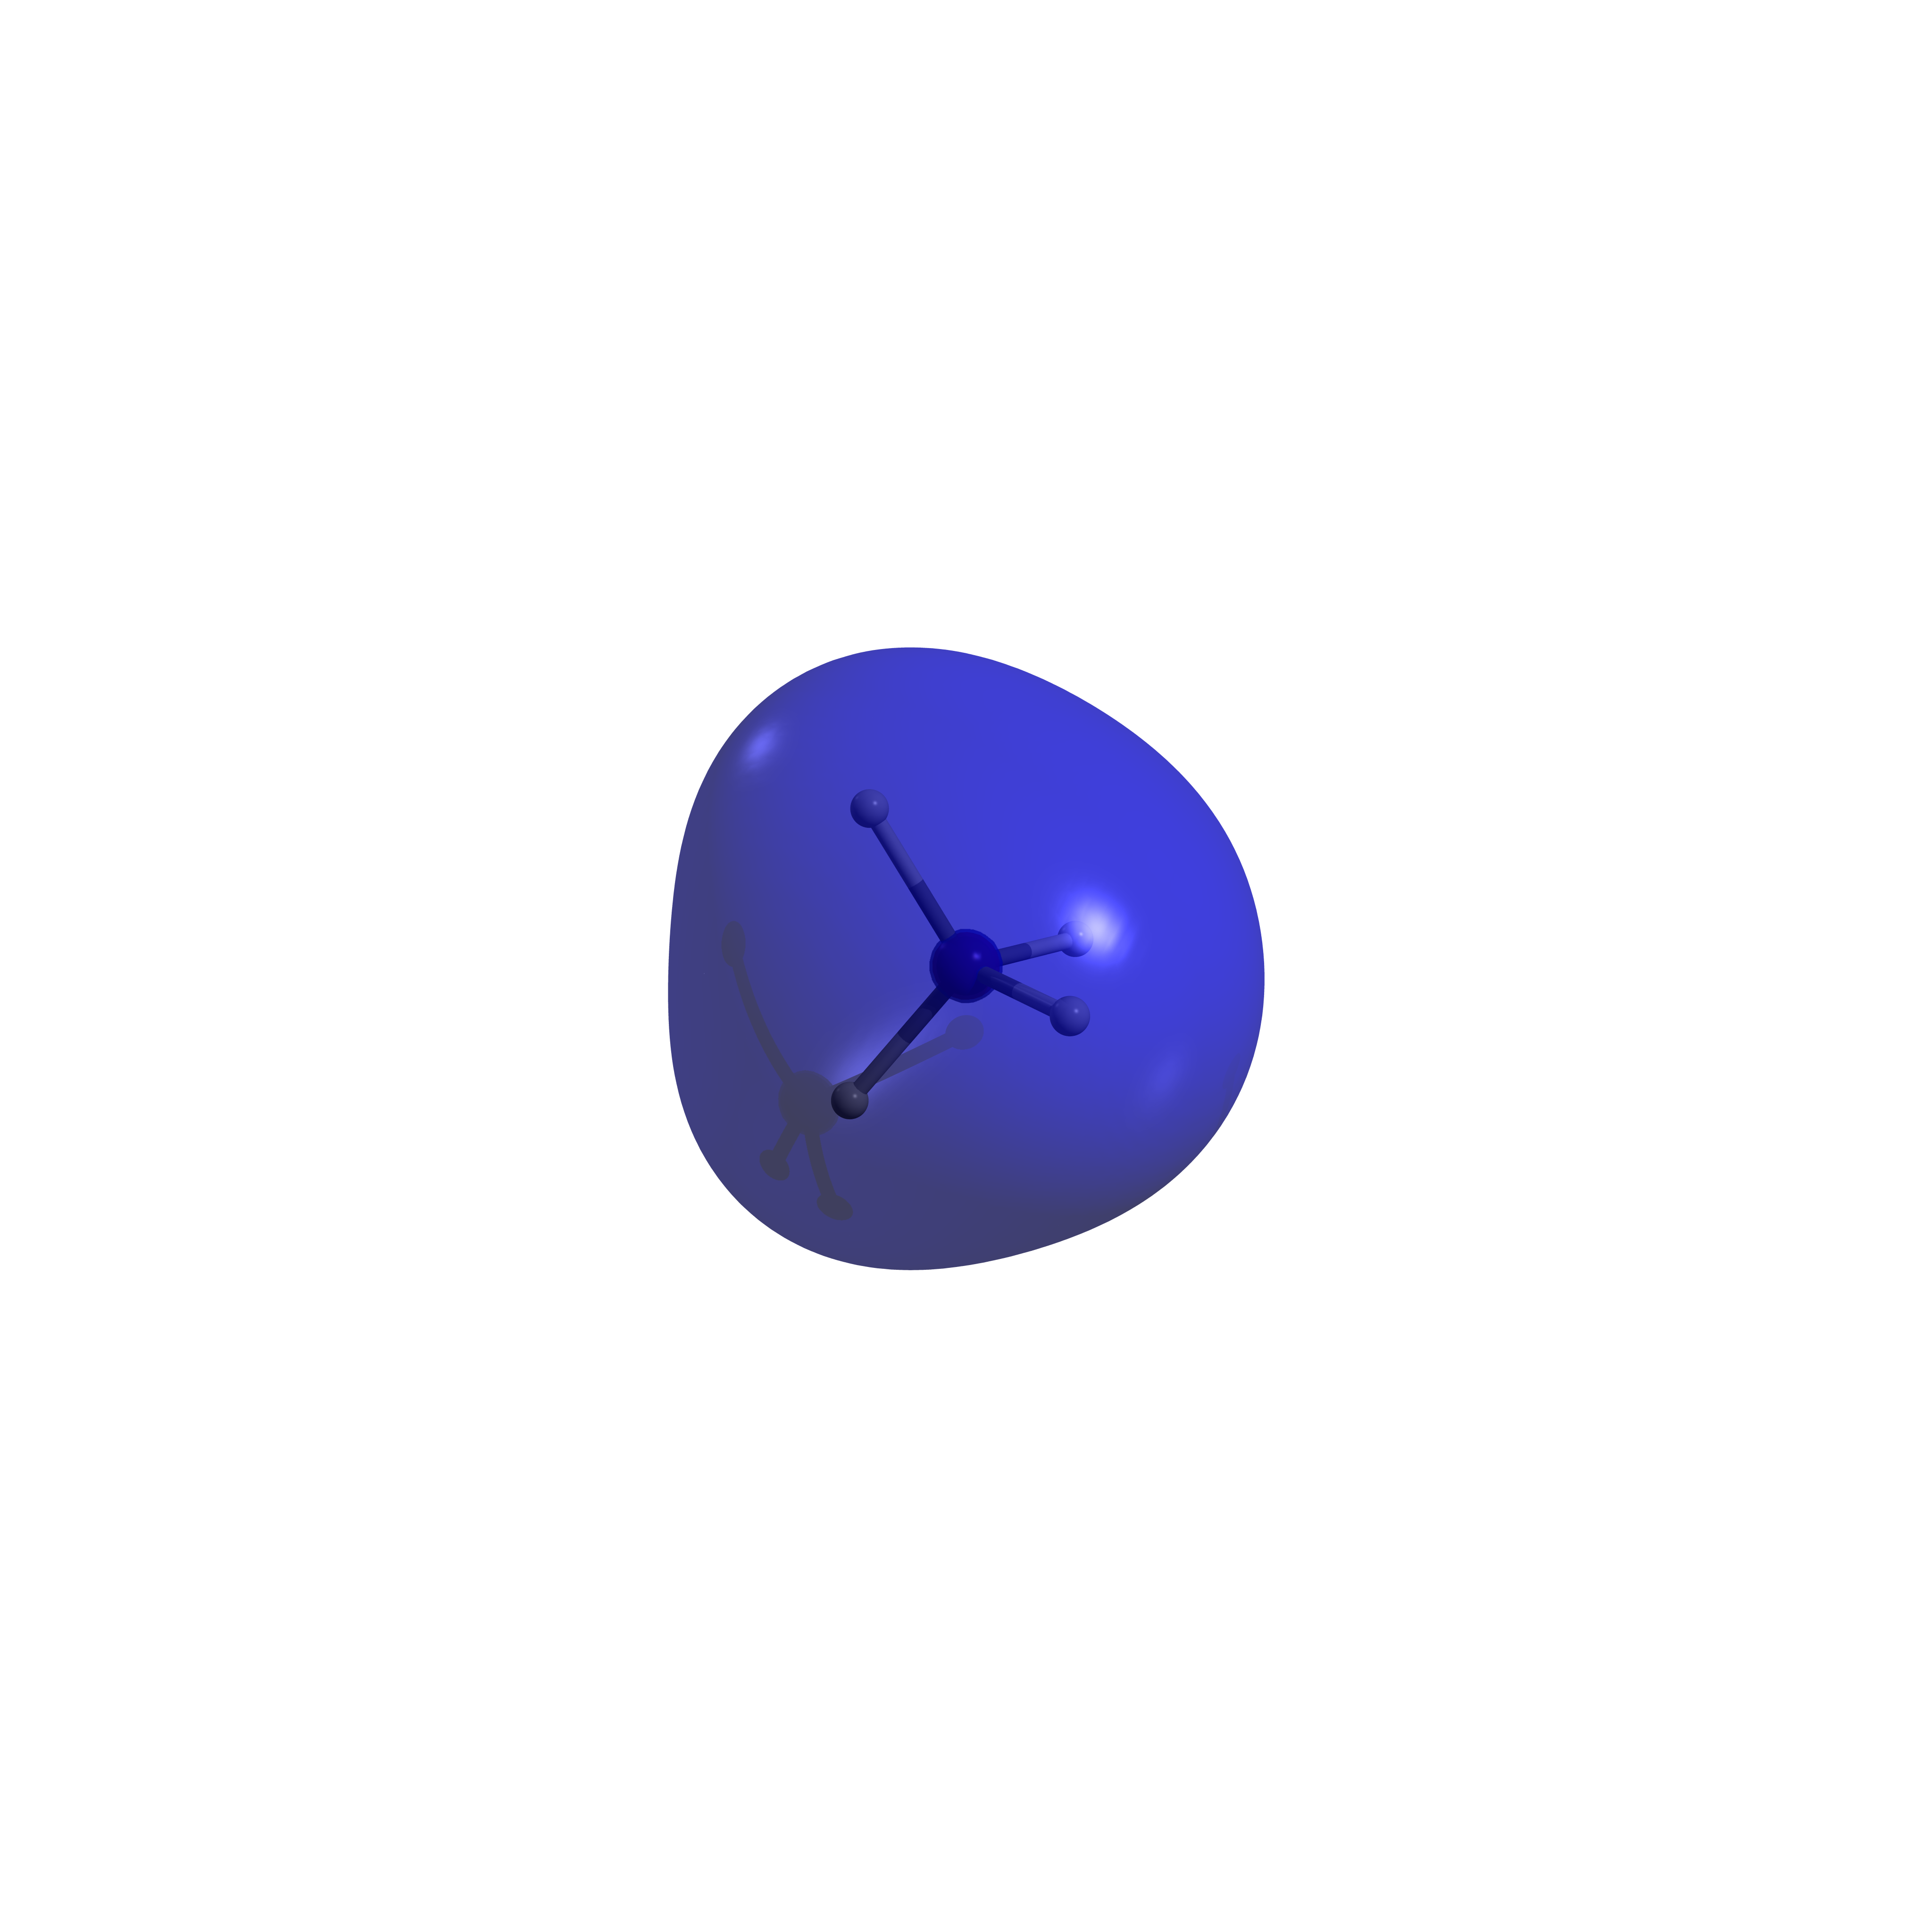
\includegraphics[trim=1200 1200 1200 1200, clip, width=0.45\textwidth]{res/CH4/ch4_w1.png}\\
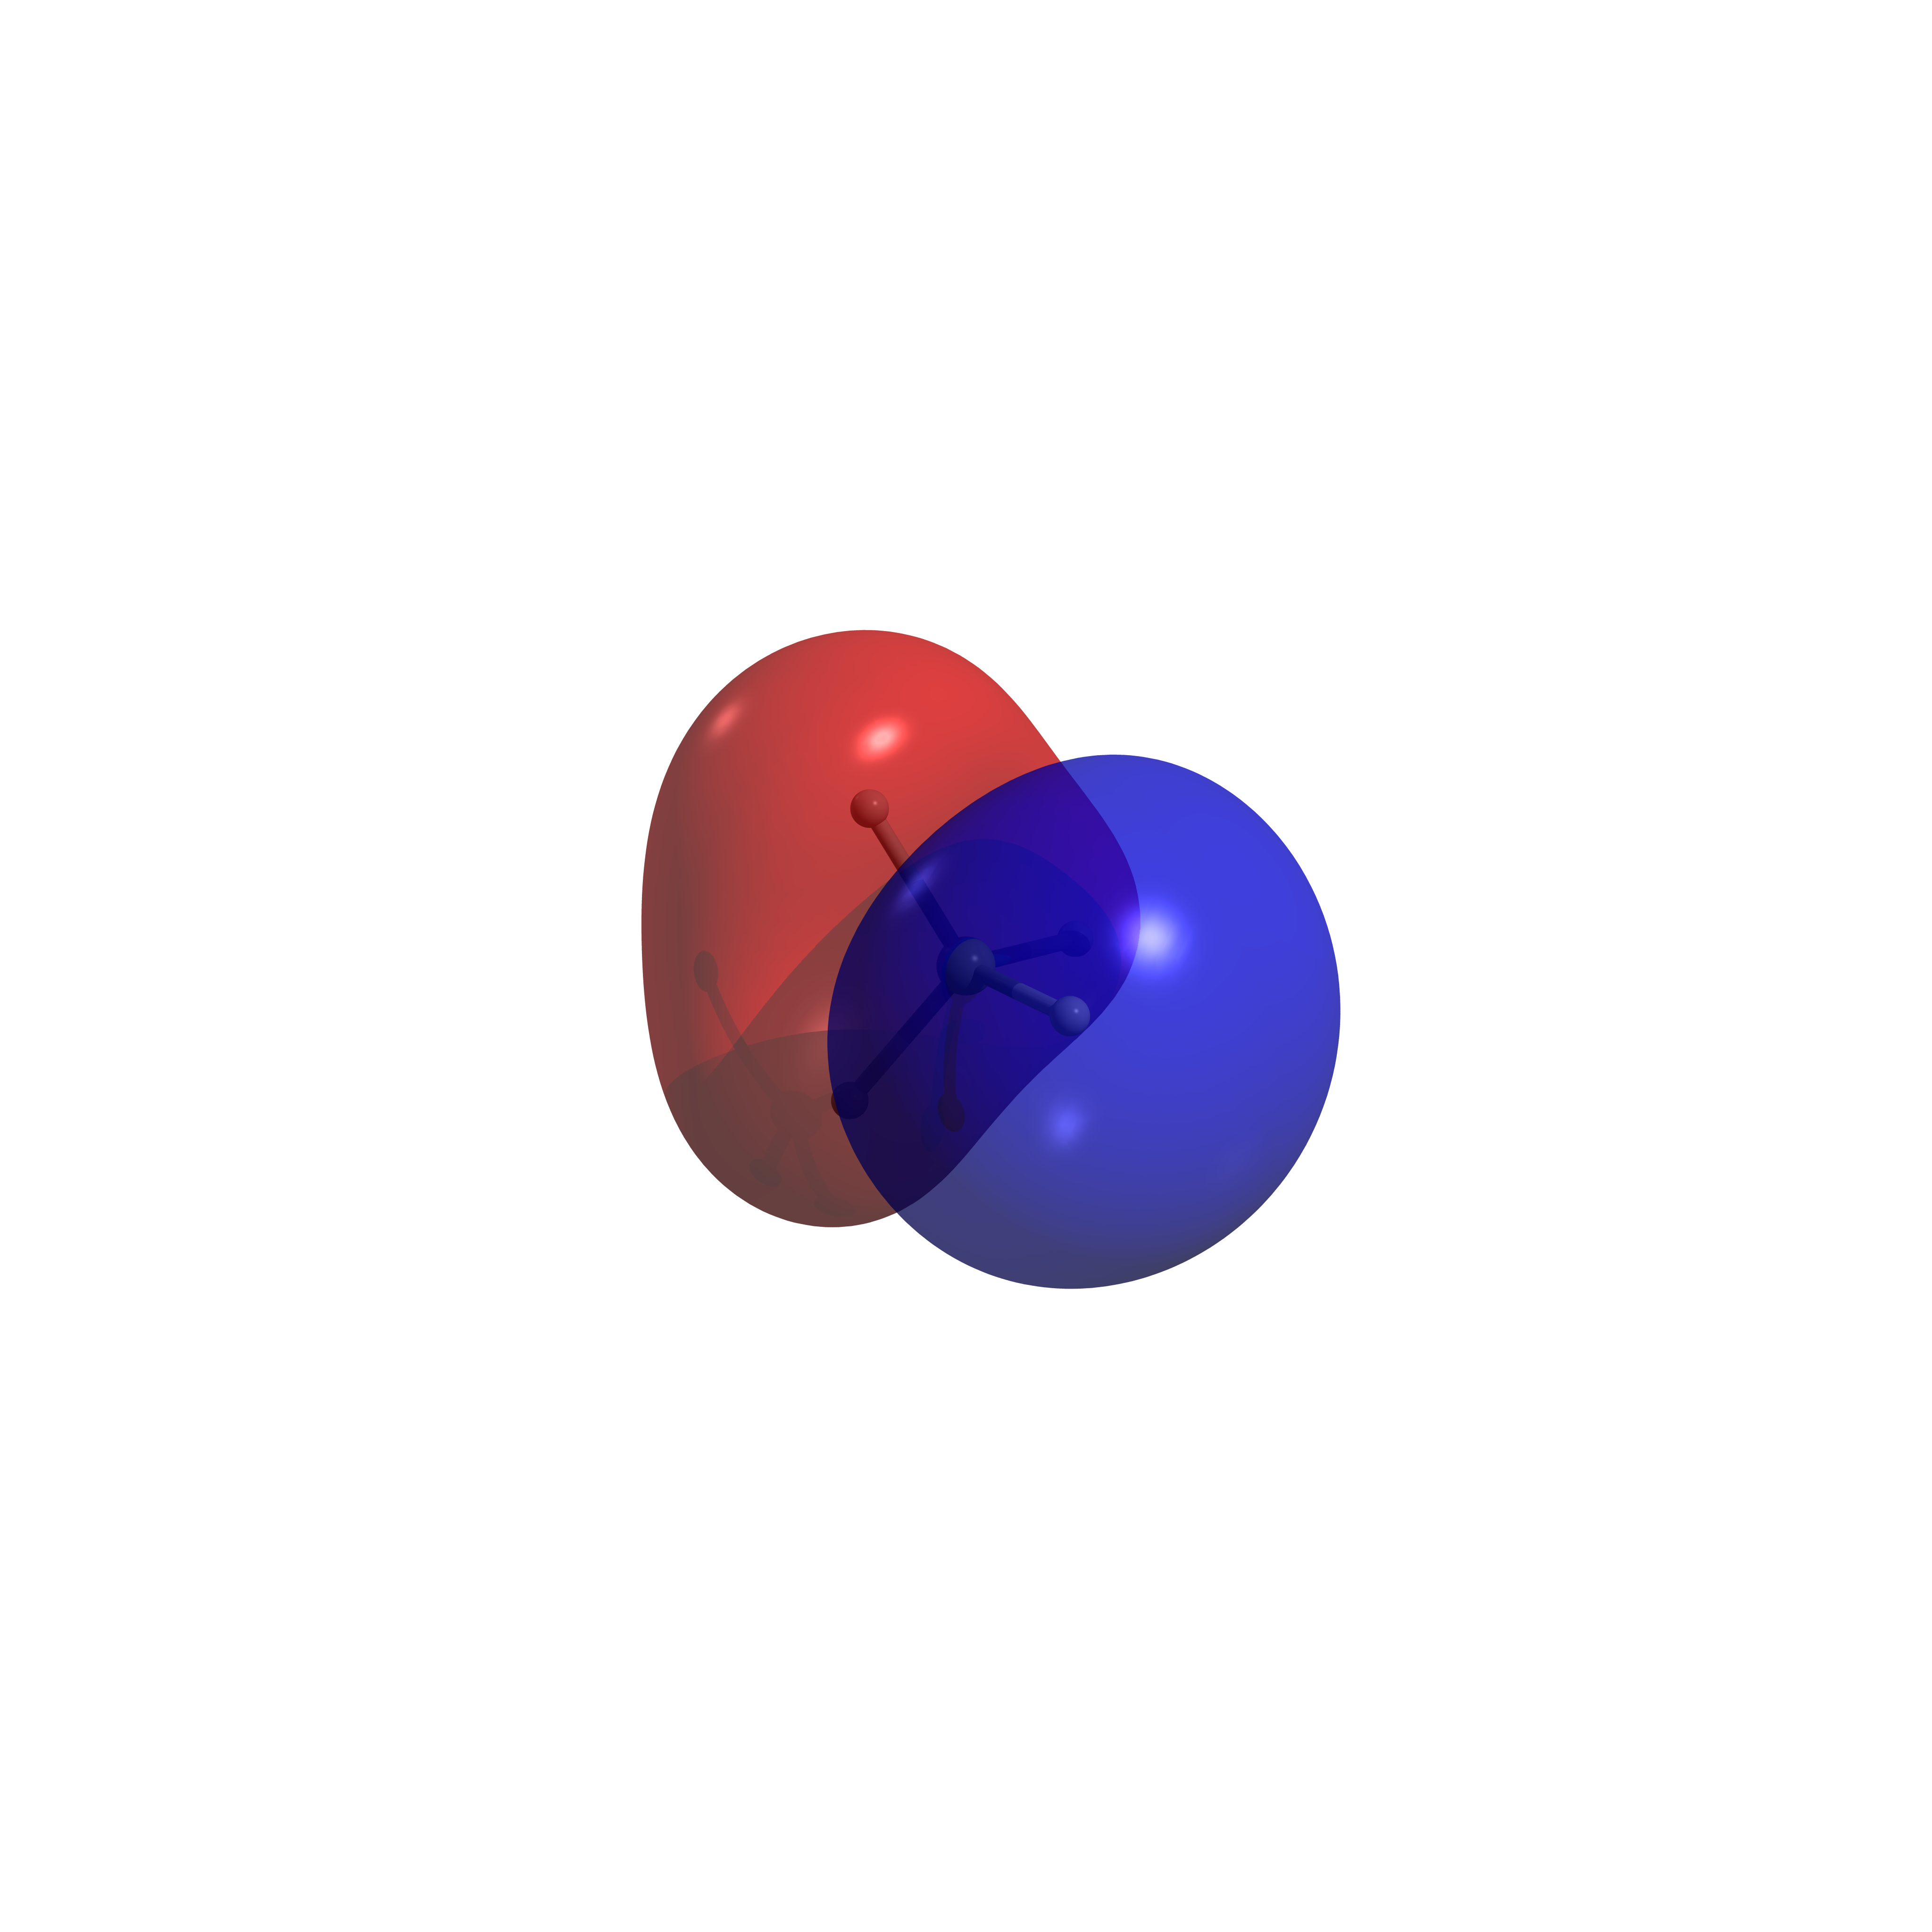
\includegraphics[trim=1200 1200 1200 1200, clip, width=0.45\textwidth]{res/CH4/ch4_w2.png}
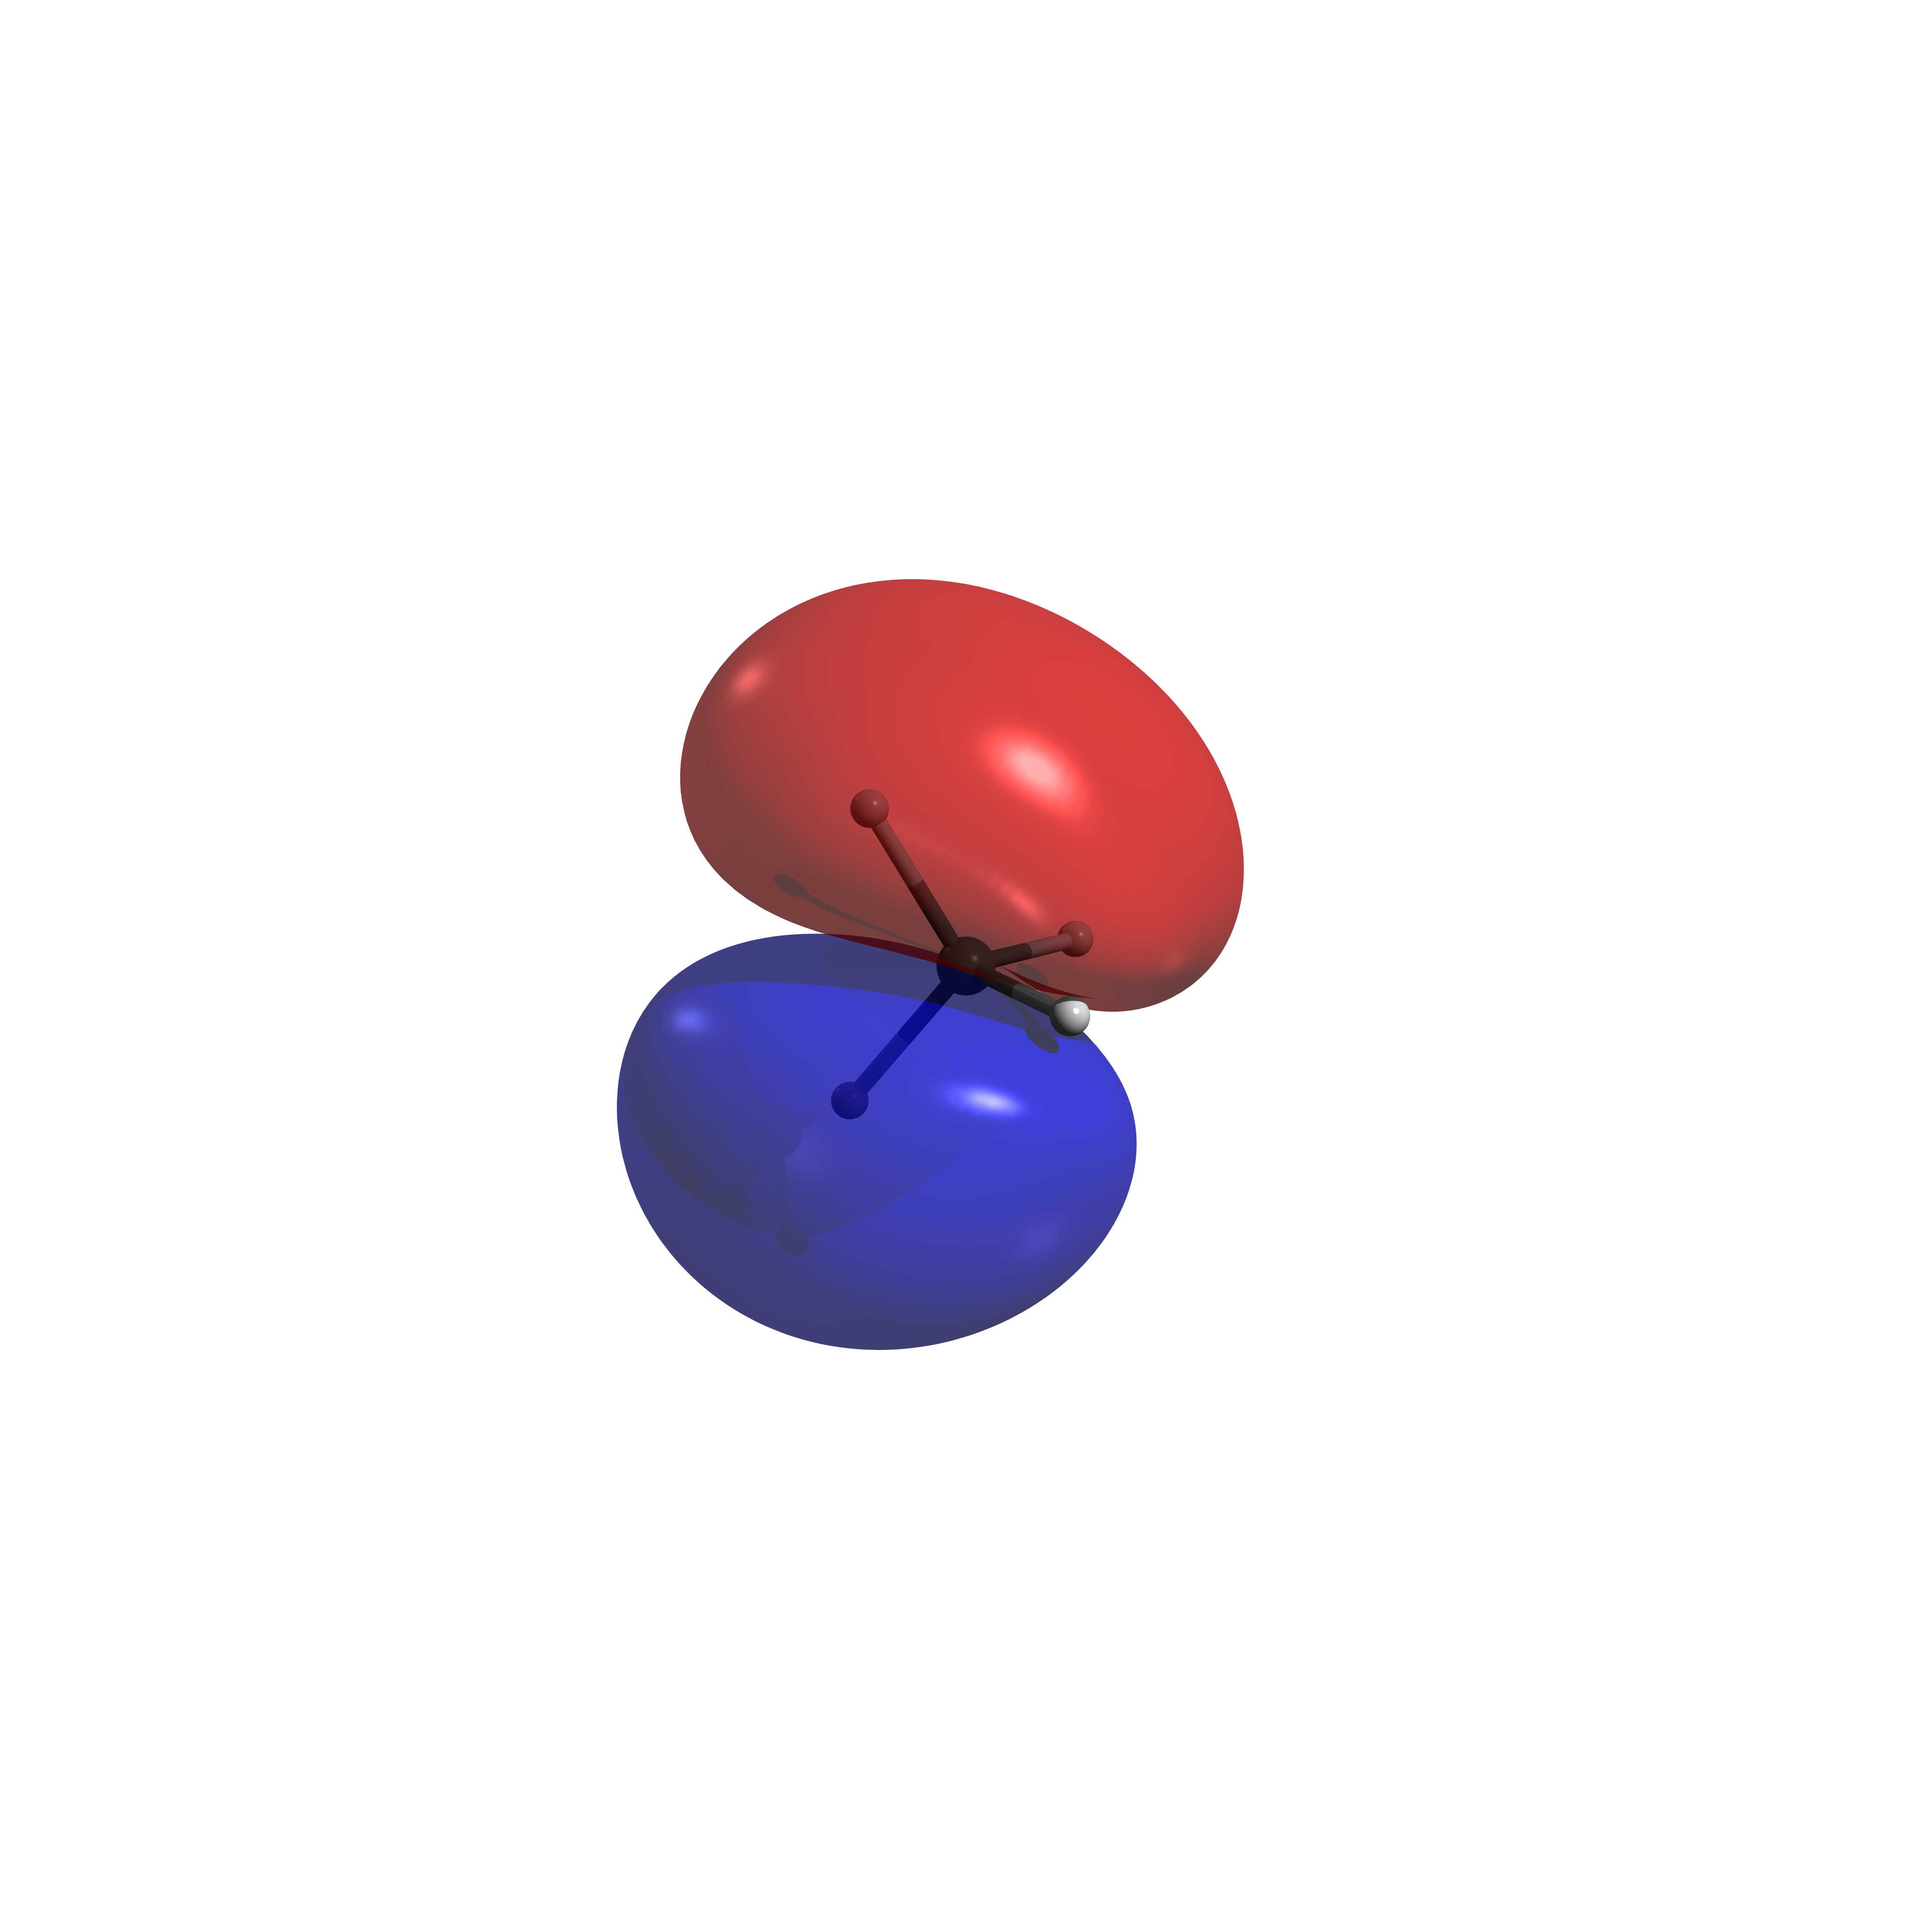
\includegraphics[trim=1200 1200 1200 1200, clip, width=0.45\textwidth]{res/CH4/ch4_w3.png}\\
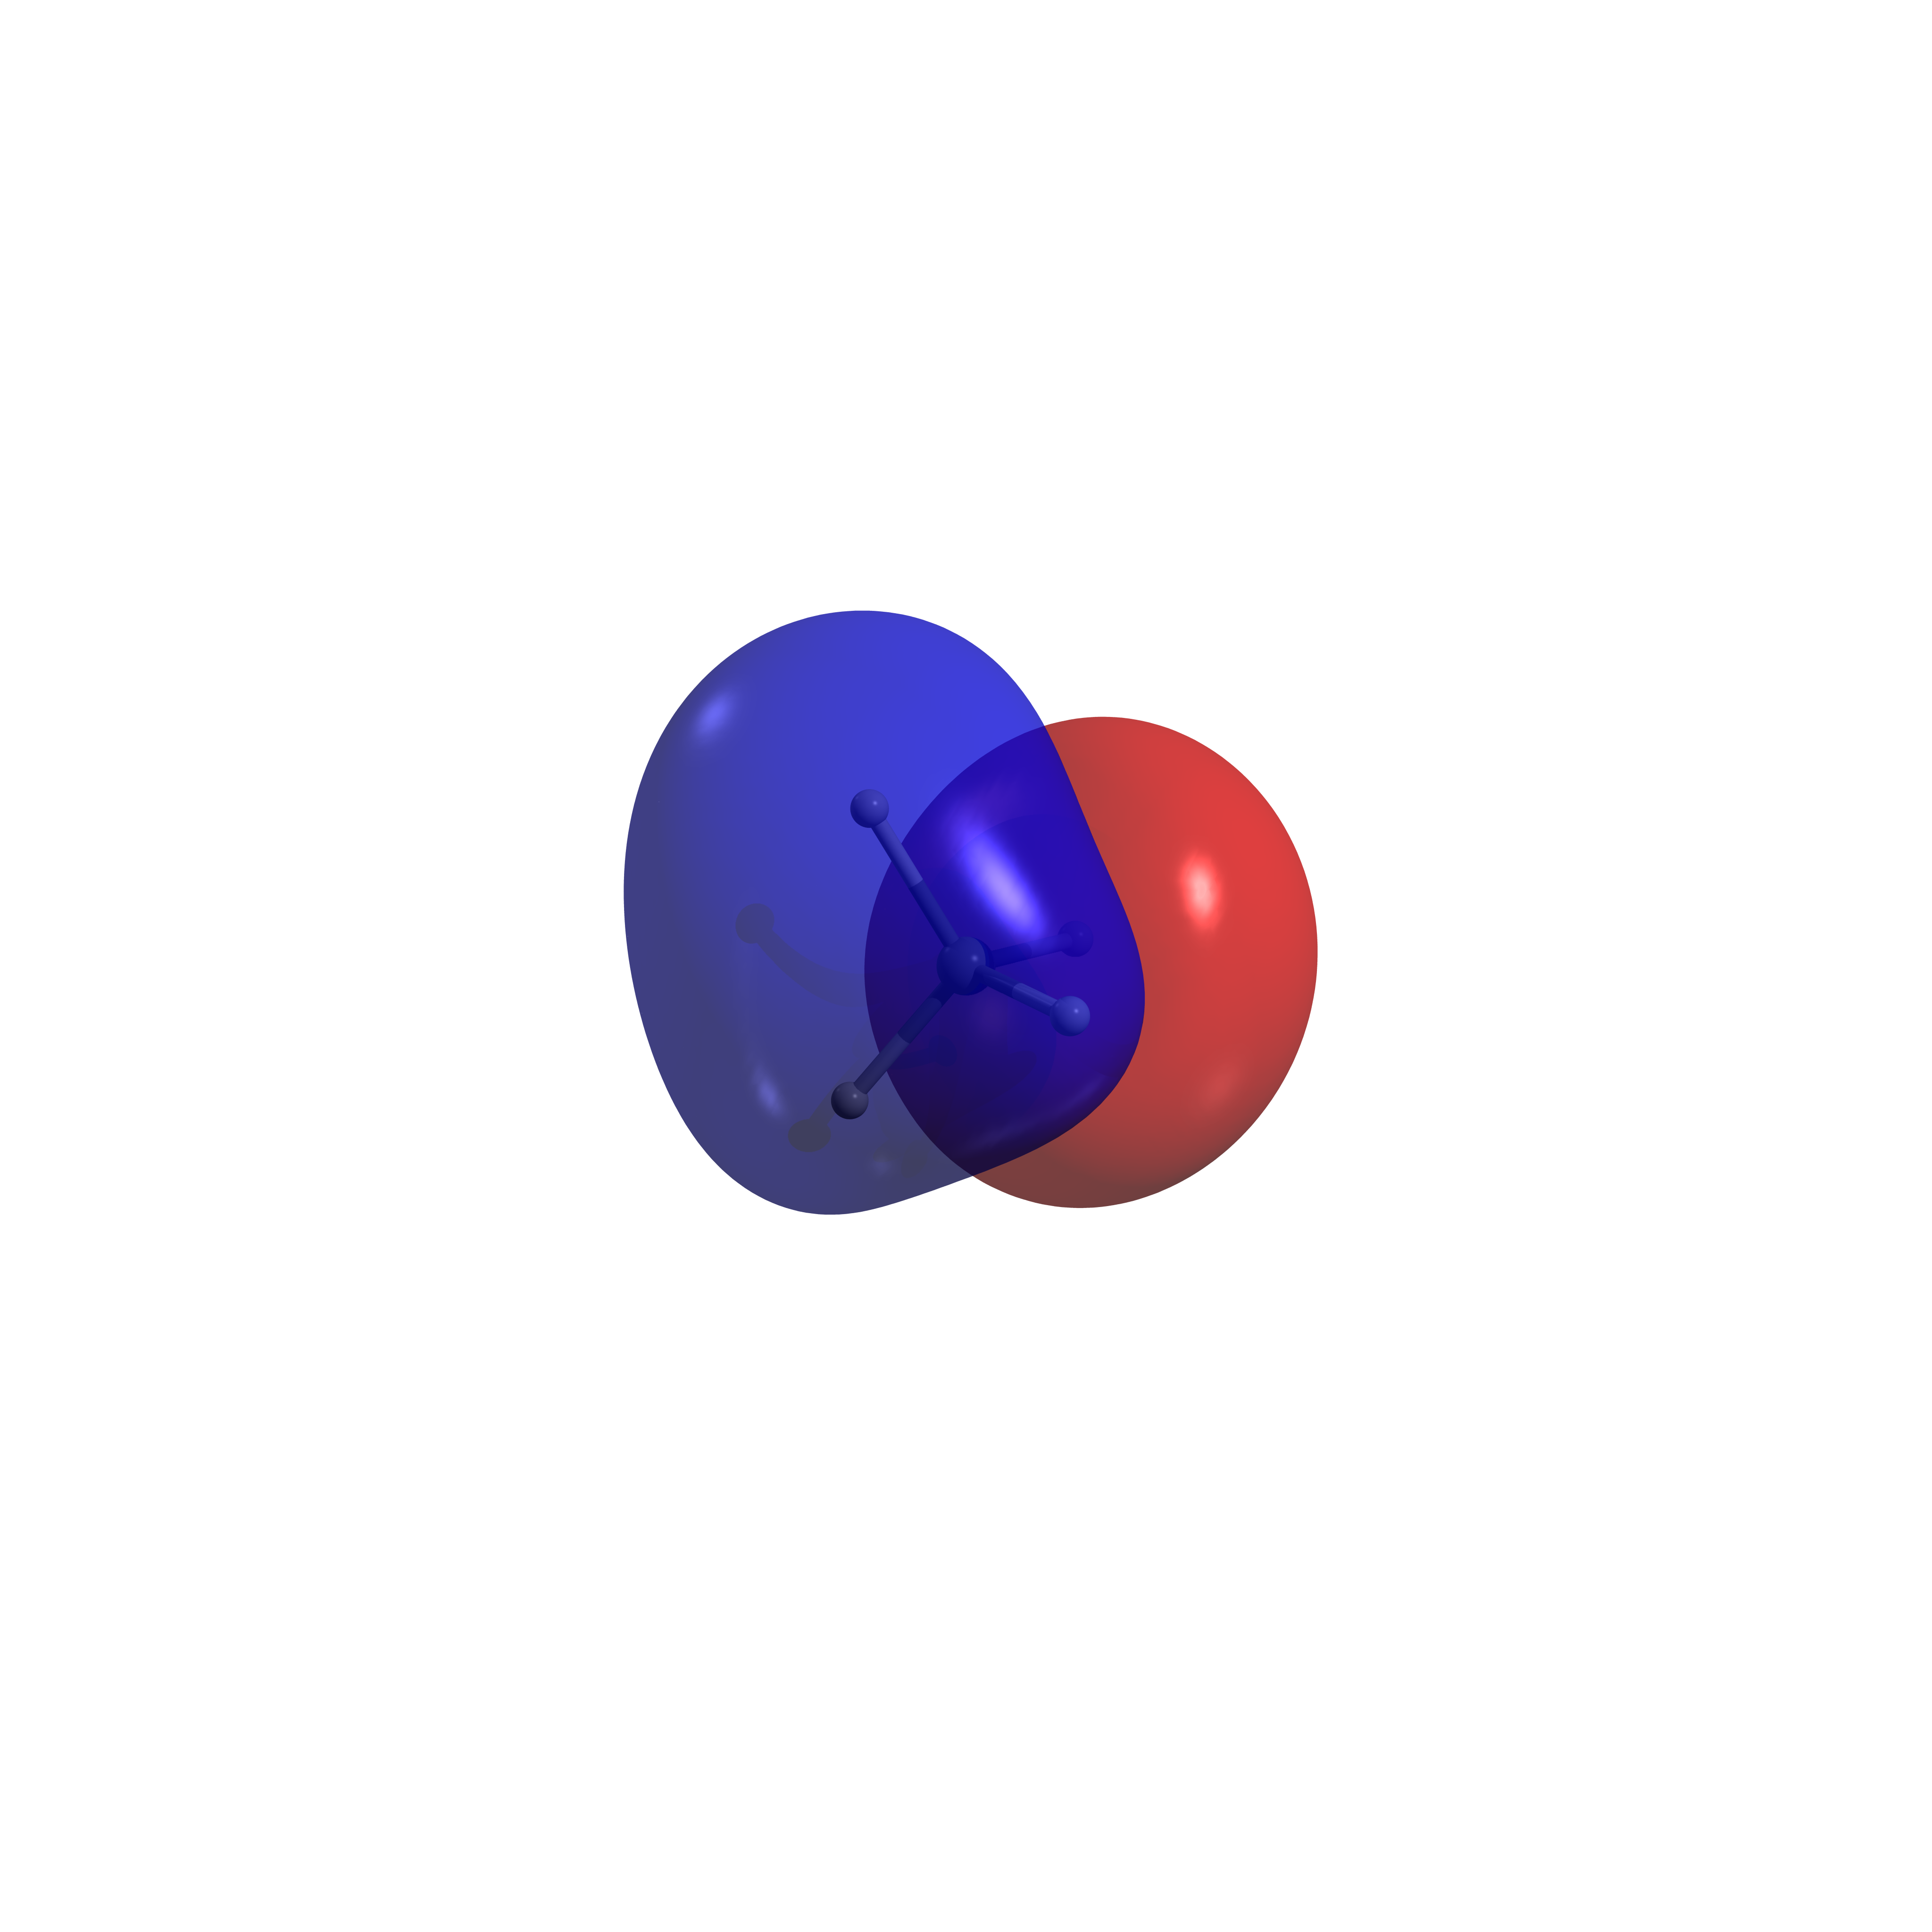
\includegraphics[trim=1200 1200 1200 1200, clip, width=0.45\textwidth]{res/CH4/ch4_w4.png}
\caption{Die fünf besetzten Orbitale des CH$_4$\-/Moleküls,
nach aufsteigender Energie sortiert.
\textcolor{blue}{$\blacksquare$} positiv,
\textcolor{red}{$\blacksquare$} negativ.}\label{ch4_orbitals}
\end{figure}

\end{enumerate}